%_____________________________________________________________________________
%=============================================================================
% main.tex v8 (31-05-2015) \ldots dibuat oleh Lionov - Informatika FTIS UNPAR
% 
% Ini adalah file utama (main.tex), berisi perintah-perintah yang khusus 
% dibuat untuk template ini
%
% 			JANGAN MENGUBAH APAPUN DI DALAM FILE INI,
%			KECUALI ANDA TAHU APA YANG ANDA LAKUKAN !!!
%
% Jika ada tambahan perintah, dapat anda tuliskan di tempat yang telah disediakan 
% di baris 310 pada file ini
% Jika daftar tabel tidak digunakan, anda harus menghapus (beri komentar) secara
% manual di baris 485
%
% Bug, kritik, saran: silahkan kirimkan via email ke lionov@unpar.ac.id
%
% Perubahan pada versi 8 (31-05-2015):
%	- penambahan default data untuk beberapa keterangan dan digunakan sebagai 
%	  template dengan tanda << & >> . Data yang diubah defaultnya adalah: nama skripsi
%	  nama prodi, beserta bahasa inggrisnya.
%   - Keywords dan kata kunci di abstrak ditambahkan noindent + perbaikan lainnya
%   - Perbaikan untuk halaman tidak kosong tanpa nomor halaman romawi
%
% Perubahan pada versi sebelumnya :
%	versi 7 (27-05-2014)
%	- penambahan perintah \raggedbottom untuk menghilangkan area kosong akibat 
%	  penempatan gambar yang tidak sempurna
%	versi 6 (10-11-2013)
%	- perbaikan pada abstract dengan paragraf lebih dari satu: perbaikan vertical spacing
%	- perbaikan pada tampilan bab dan lampiran: tidak perlu menuliskan apapun untuk 
%	  menampilkan semuanya (di data.tex) atau -1 jika tidak ada lampiran
%	- halaman bernomor genap untuk halaman romawi sudah dimunculkan
%	- Kurikulum 2013 : perubahan nama buku skripsi 
%	versi 5 (21-10-2012)
%	- halaman terakhir setiap bab tidak ada headernya jika kosong
%	versi 4 (06-08-2012)
% 	- penggabungan main.tex, depan.tex dan setup.tex menjadi main.tex
% 	- menambahkan keterangan di lampiran untuk kode program 
% 	- ukuran font dapat diubah langsung di tiap lampiran
% 	versi 3 (09-07-2012): 
%	- Tidak ada di file ini
% 	versi 2 :
% 	- "Daftar Referensi" tidak perlu diubah secara manual (tidak perlu mengubah file bahasai.ldf)
% 	- Bahasa Indonesia dari abstract adalah abstrak (secara otomatis), bukan ringkasan
% 	- Spasi pada buku dokumen final adalah onehalfspacing
%
% to do : - hilangkan secara otomatis daftar tabel/gambar jika tidak digunakan
%         - (IT) aturan penulisan algoritma untuk IT (pakai algo.sty ?)
%=============================================================================

%=============================================================================
% setup.tex v2 (08-07-2012)
% Perubahan pada versi 2:
% - Menambahkan perintah untuk judulINA dan judulENG
% - Menghapus \usepackage{microtype}, yang pada beberapa kasus menjadi masalah
%=============================================================================
% depan.tex v2 (09-07-2012)
% Perubahan pada versi 2:
% - Menambahkan halaman depan dalam bahasa inggris
%=============================================================================

%setup.tex
\documentclass[11pt,a4paper,twoside,openright,notitlepage]{report} 

\usepackage[bahasa]{babel} %bahasa indonesia
\usepackage[T1]{fontenc}  %encoding
% \usepackage{mathptmx}
% \usepackage{venturisold}
% \usepackage{helvet}
% \usepackage{fouriernc} 
\usepackage{abstract} %manipulasi abstract
\usepackage{chappg} % format daftar isi 
\usepackage{color} %warna
\usepackage{etoolbox} %untuk programming if-then
\usepackage{fancyhdr} %format header & footer
\usepackage{float} %penempatan gambar di tempat yg seharusnya
\usepackage[inner=2.5cm,outer=2cm,top=2.5cm,bottom=2.5cm]{geometry} %margin
\usepackage{graphicx} %gambar
\usepackage{listings} %source code
\usepackage{lscape} %landscape untuk source code
\usepackage{multicol} %multiple column
\usepackage{ifthen} % if then
\usepackage[pagewise]{lineno} %line numbering
\usepackage{lipsum} % untuk testing
\usepackage{titlesec} %judul header
\usepackage{tocbibind} %daftar isi, gambar, tabel dll
\usepackage{tocloft} % format daftar isi 
\usepackage{setspace} %line spacing
\usepackage{xstring} %manipulasi string
\usepackage[plainpages=false,pdfpagelabels,unicode]{hyperref} %\autoref, \phantomsection & link 
\usepackage{emptypage}

\usepackage{caption}
\usepackage{enumitem}
\usepackage{rotating}
\usepackage{algorithmicx}
\usepackage{algorithm}
\usepackage{algpseudocode}

\let\abstractname\Abstrak

\titleformat{\chapter}[display] {\Large\bfseries\centering}{\MakeUppercase{\chaptertitlename} \thechapter}{15pt}{\Large\MakeUppercase}

\renewcommand{\cftchapfont}{\scshape \bfseries}

\renewcommand{\cfttoctitlefont}{\hfil\Large\bfseries\MakeUppercase}
\renewcommand{\cftaftertoctitle}{\hfill}
\renewcommand{\cftloftitlefont}{\hfill\Large\bfseries\MakeUppercase}
\renewcommand{\cftafterloftitle}{\hfill}
\renewcommand{\cftlottitlefont}{\hfill\Large\bfseries\MakeUppercase}
\renewcommand{\cftafterlottitle}{\hfill}

% Tidak perlu ada kata "Bab", "Gambar" atau "Tabel" di daftar 
% \renewcommand{\cftchappresnum}{{\bf \scshape Bab} } 
% \renewcommand{\cftchapnumwidth}{1.5cm}
% \renewcommand{\cftfigpresnum}{{Gambar\ }} 
% \renewcommand{\cftfignumwidth}{2.5cm}
% \renewcommand{\cfttabpresnum}{{Tabel\ }} 
% \renewcommand{\cfttabnumwidth}{2cm}

\newcommand{\apptoc}{
	% Hapus kata "Lampiran" dari daftar isi
	%\addtocontents{toc}{\protect\renewcommand{\protect\cftchappresnum}{\bf \scshape Lampiran\  }}%
	%\addtocontents{toc}{\protect\renewcommand{\protect\cftchapnumwidth}{2.75cm}}
	\addtocontents{toc}{\protect\renewcommand{\protect\cftchappresnum}{\bf \scshape}}%	

}

\newcommand{\vnama}{Jane Doe}
\newcommand{\vlnama}{John Doe}
\newcommand{\vnpm}{1992700001}
\newcommand{\vprodiINA}{SAINS}
\newcommand{\vprodiENG}{SCIENCE}
\newcommand{\vstaINA}{UJIAN}
\newcommand{\vstaENG}{EXAM}
%\newcommand{\vjudul}{Judul Skripsi/Tugas Akhir}
\newcommand{\vpembu}{Plato}
\newcommand{\vpembs}{Euclid}
\newcommand{\vpengi}{Plato}
\newcommand{\vpengii}{Euclid}
\newcommand{\vtanggal}{1}
\newcommand{\vbulan}{Januari}
\newcommand{\vtahun}{1970}
\newcommand{\vmode}{final}
\newcommand{\vspacing}{double}
\newcommand{\vlineno}{yes}
\newcommand{\vkunciina}{Skripsi, Tugas Akhir}
\newcommand{\vkuncieng}{Undergraduate Thesis, Final Project}
\newcommand{\vkajur}{Jack Doe}
\newcommand{\vkajurmat}{Jack Doe}
\newcommand{\vkajurfis}{Jack Doe}
\newcommand{\vkajurtif}{Jack Doe}

\newcommand{\namanpm}[2]{
	\renewcommand{\vstaINA}{<<SKRIPSI/TUGAS AKHIR>>}
	\renewcommand{\vprodiINA}{<<MATEMATIKA/FISIKA/TEKNIK INFORMATIKA>>}
	\renewcommand{\vstaENG}{<<FINAL PROJECT/UNDERGRADUATE THESIS>>}
	\renewcommand{\vprodiENG}{<<MATHEMATICS/PHYSICS/INFORMATICS>>}
	\renewcommand{\vnama}{\uppercase{#1}} \renewcommand{\vlnama}{#1} \hypersetup{pdfauthor={#2 - #1}}
	\renewcommand{\vnpm}{#2} \hypersetup{pdfcreator={#2}} \StrChar{\vnpm}{6}[\vprodiN]
	\ifdefstring{\vprodiN}{1}{
		\renewcommand{\vprodiINA}{MATEMATIKA} \renewcommand{\vprodiENG}{MATHEMATICS} 
		\renewcommand{\vstaINA}{SKRIPSI} \renewcommand{\vstaENG}{FINAL PROJECT} \renewcommand{\vkajur}{\vkajurmat}}{}
	\ifdefstring{\vprodiN}{2}{
		\renewcommand{\vprodiINA}{FISIKA} \renewcommand{\vprodiENG}{PHYSICS} 
		\renewcommand{\vstaINA}{TUGAS AKHIR} \renewcommand{\vstaENG}{FINAL PROJECT} \renewcommand{\vkajur}{\vkajurfis}}{}
	\ifdefstring{\vprodiN}{3}{
		\renewcommand{\vprodiINA}{TEKNIK INFORMATIKA} \renewcommand{\vprodiENG}{INFORMATICS} 
		\renewcommand{\vstaINA}{SKRIPSI} \renewcommand{\vstaENG}{UNDERGRADUATE THESIS} \renewcommand{\vkajur}{\vkajurtif}}{}}

%\newcommand{\judul}[1]{\renewcommand{\vjudul}{\uppercase{#1}}\hypersetup{pdftitle={#1}, pdfsubject={#1}}}
\newcommand{\pembimbing}[2]{\renewcommand{\vpembu}{#1}\renewcommand{\vpembs}{#2}}
\newcommand{\penguji}[2]{\renewcommand{\vpengi}{#1}\renewcommand{\vpengii}{#2}}
\newcommand{\kajur}[3]{\renewcommand{\vkajurmat}{#1}\renewcommand{\vkajurfis}{#2}\renewcommand{\vkajurtif}{#3}}
\renewcommand{\vbulan}{<<bulan>>}
\newcommand{\tanggal}[3]{\renewcommand{\vtanggal}{#1}\renewcommand{\vtahun}{#3}
	\newcommand{\vcbulan}{#2}
	\ifdefstring{\vcbulan}{1}{\renewcommand{\vbulan}{Januari}}{}
	\ifdefstring{\vcbulan}{2}{\renewcommand{\vbulan}{Februari}}{}
	\ifdefstring{\vcbulan}{3}{\renewcommand{\vbulan}{Maret}}{}
	\ifdefstring{\vcbulan}{4}{\renewcommand{\vbulan}{April}}{}
	\ifdefstring{\vcbulan}{5}{\renewcommand{\vbulan}{Mei}}{}
	\ifdefstring{\vcbulan}{6}{\renewcommand{\vbulan}{Juni}}{}
	\ifdefstring{\vcbulan}{7}{\renewcommand{\vbulan}{Juli}}{}
	\ifdefstring{\vcbulan}{8}{\renewcommand{\vbulan}{Agustus}}{}
	\ifdefstring{\vcbulan}{9}{\renewcommand{\vbulan}{September}}{}
	\ifdefstring{\vcbulan}{10}{\renewcommand{\vbulan}{Oktober}}{}
	\ifdefstring{\vcbulan}{11}{\renewcommand{\vbulan}{November}}{}
	\ifdefstring{\vcbulan}{12}{\renewcommand{\vbulan}{Desember}}{}	
}

\newcommand{\judulINA}[1]{\newcommand{\vjudulINA}{\uppercase{#1}}\hypersetup{pdftitle={#1},pdfsubject={#1}}}
\newcommand{\judulENG}[1]{\newcommand{\vjudulENG}{\uppercase{#1}}\hypersetup{pdftitle={#1},pdfsubject={#1}}}
\newcommand{\abstrakINA}[1]{\newcommand{\vabstrakina}{#1}}
\newcommand{\abstrakENG}[1]{\newcommand{\vabstrakeng}{#1}}
\newcommand{\kunciINA}[1]{\renewcommand{\vkunciina}{#1} \hypersetup{pdfkeywords={#1}}}
\newcommand{\kunciENG}[1]{\renewcommand{\vkuncieng}{#1}}
\newcommand{\untuk}[1]{\newcommand{\vuntuk}{#1}}
\newcommand{\prakata}[1]{\newcommand{\vprakata}{#1}}
\newcommand{\mode}[1]{\renewcommand{\vmode}{#1}}
\newcommand{\linespacing}[1]{\renewcommand{\vspacing}{#1}}
\newcommand{\linenumber}[1]{\renewcommand{\vlineno}{#1}}

\newcommand{\bab}[1]{\newcommand{\vbab}{#1}}
\newcommand{\lampiran}[1]{\renewcommand{\vlmp}{#1}}

\newcommand{\vpilbab}{0}
\newcommand{\vbaba}{0}\newcommand{\vbabb}{0}\newcommand{\vbabc}{0}
\newcommand{\vbabd}{0}\newcommand{\vbabe}{0}\newcommand{\vbabf}{0}
\newcommand{\vbabg}{0}\newcommand{\vbabh}{0}\newcommand{\vbabi}{0}
\newcommand{\vpillmp}{0}
\newcommand{\vlmpa}{0}\newcommand{\vlmpb}{0}\newcommand{\vlmpc}{0}
\newcommand{\vlmpd}{0}\newcommand{\vlmpe}{0}\newcommand{\vlmpf}{0}
\newcommand{\vlmpg}{0}\newcommand{\vlmph}{0}\newcommand{\vlmpi}{0}
\newcommand{\vlmp}{x}

%	\ifdefempty{#1}{\bab{1,2,3,4,5,6,7,8,9} \tampilbab{\vbab}}{
\newcommand{\tampilbab}[1]{
	\ifdefempty{#1}{
		\renewcommand{\vbaba}{1}\renewcommand{\vbabb}{1}\renewcommand{\vbabc}{1}
		\renewcommand{\vbabd}{1}\renewcommand{\vbabe}{1}\renewcommand{\vbabf}{1}
		\renewcommand{\vbabg}{1}\renewcommand{\vbabh}{1}\renewcommand{\vbabi}{1}}{
	\renewcommand{\do}[1]{
		\renewcommand{\vpilbab}{##1}
		\ifdefstring{\vpilbab}{1}{\renewcommand{\vbaba}{1}}{}
		\ifdefstring{\vpilbab}{2}{\renewcommand{\vbabb}{1}}{}
		\ifdefstring{\vpilbab}{3}{\renewcommand{\vbabc}{1}}{}
		\ifdefstring{\vpilbab}{4}{\renewcommand{\vbabd}{1}}{}
		\ifdefstring{\vpilbab}{5}{\renewcommand{\vbabe}{1}}{}
		\ifdefstring{\vpilbab}{6}{\renewcommand{\vbabf}{1}}{}
		\ifdefstring{\vpilbab}{7}{\renewcommand{\vbabg}{1}}{}
		\ifdefstring{\vpilbab}{8}{\renewcommand{\vbabh}{1}}{}
		\ifdefstring{\vpilbab}{9}{\renewcommand{\vbabi}{1}}{}
	}
	\expandafter\docsvlist\expandafter{#1}
	}
}

\newcommand{\tampillmp}[1]{
	\ifdefempty{#1}{
		\renewcommand{\vlmpa}{1}\renewcommand{\vlmpb}{1}\renewcommand{\vlmpc}{1}
		\renewcommand{\vlmpd}{1}\renewcommand{\vlmpe}{1}\renewcommand{\vlmpf}{1}
		\renewcommand{\vlmpg}{1}\renewcommand{\vlmph}{1}\renewcommand{\vlmpi}{1}}{
	\ifdefstring{#1}{-1}{ }{
		\renewcommand{\do}[1]{ 
			\renewcommand{\vpillmp}{##1}
			\ifdefstring{\vpillmp}{A}{\renewcommand{\vlmpa}{1}}{}
			\ifdefstring{\vpillmp}{B}{\renewcommand{\vlmpb}{1}}{}
			\ifdefstring{\vpillmp}{C}{\renewcommand{\vlmpc}{1}}{}
			\ifdefstring{\vpillmp}{D}{\renewcommand{\vlmpd}{1}}{}
			\ifdefstring{\vpillmp}{E}{\renewcommand{\vlmpe}{1}}{}
			\ifdefstring{\vpillmp}{F}{\renewcommand{\vlmpf}{1}}{}
			\ifdefstring{\vpillmp}{G}{\renewcommand{\vlmpg}{1}}{}
			\ifdefstring{\vpillmp}{H}{\renewcommand{\vlmph}{1}}{}
			\ifdefstring{\vpillmp}{I}{\renewcommand{\vlmpi}{1}}{}}
		}
	\expandafter\docsvlist\expandafter{#1}
	}
}

\newcommand{\appspacing}{
	\ifdefstring{\vspacing}{single}{\singlespacing}{}
	\ifdefstring{\vspacing}{onehalf}{\onehalfspacing}{}
	\ifdefstring{\vspacing}{double}{\doublespacing}{}
	\ifdefstring{\vmode}{final}{\onehalfspacing}{}
}

\newcommand{\appline}{
	\ifdefstring{\vmode}{final}{\renewcommand{\vlineno}{no}}{}
	\ifdefstring{\vlineno}{yes}{\linenumbers \def\linenumberfont{\normalfont\tiny\sffamily}}{}
	\ifdefstring{\vlineno}{no}{\lstset{numbers=left, stepnumber=1, numbersep=5pt}}{}
	
}

\newcommand{\appmargin}{
	\ifdefstring{\vmode}{final}{}{\newgeometry{inner=3cm,outer=2.75cm,top=2cm,bottom=2cm}}
}

\renewcommand{\abstractnamefont}{\bf \MakeUppercase}

\makeatletter
\def\headrule{{%
  \if@fancyplain\let\headrulewidth\plainheadrulewidth\fi
  \hrule\@height\footrulewidth\@width\headwidth\vskip2pt%
  \hrule\@height\headrulewidth\@width\headwidth\vskip-\headrulewidth\vskip-4pt
}}
\def\footrule{}

\def\cleardoublepage{
	\clearpage
	\if@twoside \ifodd\c@page
	\else
		\hbox{}
		\vspace{\fill}
		\thispagestyle{empty}
		\newpage
	\if@twocolumn\hbox{}\newpage\fi\fi\fi}
\makeatother

\renewcommand{\headrulewidth}{1.25pt}
\renewcommand{\footrulewidth}{0.25pt}

\setlength{\headheight}{15pt}
\fancyhead[LE,RO]{\thepage}
\fancyhead[RE]{\small{\textsc{\nouppercase{\leftmark}}}}
\fancyhead[LO]{\small{\textsc{\nouppercase{\rightmark}}}}
\fancyfoot{}

\hypersetup{unicode=true,colorlinks=true,linkcolor=blue,citecolor=green,filecolor=magenta, urlcolor=cyan}

\lstset{basicstyle=\tiny, commentstyle=\color{blue}}
\lstset{frame=leftline, tabsize=4, breaklines=true}

%=============================================================================

%tambahkan perintah yang anda butuhkan di sini :

%=============================================================================
%end setup.tex

%_____________________________________________________________________________
%=============================================================================
% data.tex v6 (13-04-2015) \ldots dibuat oleh Lionov - Informatika FTIS UNPAR
%
% Perubahan pada versi 6 (13-04-2015)
% - Perubahan untuk data-data ``template" menjadi lebih generik dan menggunakan
%	tanda << dan >>
%
% Perubahan pada versi sebelumnya
% 	versi 5 (10-11-2013)
% 	- Perbaikan pada memasukkan bab : tidak perlu menuliskan apapun untuk 
%	  memasukkan seluruh bab (bagian V)
% 	- Perbaikan pada memasukkan lampiran : tidak perlu menuliskan apapun untuk
%	  memasukkan seluruh lampiran atau -1 jika tidak memasukkan apapun
%	versi 4 (21-10-2012)
%	- Data dosen dipindah ke dosen.tex agar jika ada perubahan/update data dosen
%   mahasiswa tidak perlu mengubah data.tex
%	- Perubahan pada keterangan dosen	
% 	versi 3 (06-08-2012)
% 	- Perubahan pada beberapa keterangan 
% 	versi 2 (09-07-2012):
% 	- Menambahkan data judul dalam bahasa inggris
% 	- Membuat bagian khusus untuk judul (bagian VIII)
% 	- Perbaikan pada gelar dosen
%_____________________________________________________________________________
%=============================================================================
% 								BAGIAN -
%=============================================================================
% Ini adalah file data (data.tex)
% Masukkan ke dalam file ini, data-data yang diperlukan oleh template ini
% Cara memasukkan data dijelaskan di setiap bagian
% Data yang WAJIB dan HARUS diisi dengan baik dan benar adalah SELURUHNYA !!
% Hilangkan tanda << dan >> jika anda menemukannya
%=============================================================================
%_____________________________________________________________________________
%=============================================================================
% 								BAGIAN I
%=============================================================================
% Tambahkan package2 lain yang anda butuhkan di sini
%=============================================================================
\usepackage{booktabs}
\usepackage[table]{xcolor}
\usepackage{longtable}
\usepackage{amsmath}
%=============================================================================

%_____________________________________________________________________________
%=============================================================================
% 								BAGIAN II
%=============================================================================
% Mode dokumen: menetukan halaman depan dari dokumen, apakah harus mengandung 
% prakata/pernyataan/abstrak dll (termasuk daftar gambar/tabel/isi) ?
% - kosong : tidak ada halaman depan sama sekali (untuk dokumen yang 
%            dipergunakan pada proses bimbingan)
% - cover : cover saja tanpa daftar isi, gambar dan tabel
% - sidang : cover, daftar isi, gambar, tabel (IT: UTS-UAS Seminar 
%			 dan UTS TA)
% - sidang_akhir : mode sidang + abstrak + abstract
% - final : seluruh halaman awal dokumen (untuk cetak final)
% Jika tidak ingin mencetak daftar tabel/gambar (misalkan karena tidak ada 
% isinya), edit manual di baris 439 dan 440 pada file main.tex
%=============================================================================
% \mode{kosong}
% \mode{cover}
% \mode{sidang}
%\mode{sidang_akhir}
\mode{final} 
%=============================================================================

%_____________________________________________________________________________
%=============================================================================
% 								BAGIAN III
%=============================================================================
% Line numbering: penomoran setiap baris, otomatis di-reset setiap berganti
% halaman
% - yes: setiap baris diberi nomor
% - no : baris tidak diberi nomor, otomatis untuk mode final
%=============================================================================
\linenumber{no}
%=============================================================================

%_____________________________________________________________________________
%=============================================================================
% 								BAGIAN IV
%=============================================================================
% Linespacing: jarak antara baris 
% - single: opsi yang disediakan untuk bimbingan, jika pembimbing tidak
%            keberatan (untuk menghemat kertas)
% - onehalf: default dan wajib (dan otomatis) jika ingin mencetak dokumen
%            final/untuk sidang.
% - double : jarak yang lebih lebar lagi, jika pembimbing berniat memberi 
%            catatan yg banyak di antara baris (dianjurkan untuk bimbingan)
%=============================================================================
%\linespacing{single}
\linespacing{onehalf}
%\linespacing{double}
%=============================================================================

%_____________________________________________________________________________
%=============================================================================
% 								BAGIAN V
%=============================================================================
% Bab yang akan dicetak: isi dengan angka 1,2,3 s.d 9, sehingga bisa digunakan
% untuk mencetak hanya 1 atau beberapa bab saja
% Jika lebih dari 1 bab, pisahkan dengan ',', bab akan dicetak terurut sesuai 
% urutan bab.
% Untuk mencetak seluruh bab, kosongkan parameter (i.e. \bab{ })  
% Catatan: Jika ingin menambahkan bab ke-10 dan seterusnya, harus dilakukan 
% secara manual
%=============================================================================
\bab{ }
%=============================================================================

%_____________________________________________________________________________
%=============================================================================
% 								BAGIAN VI
%=============================================================================
% Lampiran yang akan dicetak: isi dengan huruf A,B,C s.d I, sehingga bisa 
% digunakan untuk mencetak hanya 1 atau beberapa lampiran saja
% Jika lebih dari 1 lampiran, pisahkan dengan ',', lampiran akan dicetak 
% terurut sesuai urutan lampiran
% Jika tidak ingin mencetak lampiran apapun, isi dengan -1 (i.e. \lampiran{-1})
% Untuk mencetak seluruh mapiran, kosongkan parameter (i.e. \lampiran{ })  
% Catatan: Jika ingin menambahkan lampiran ke-J dan seterusnya, harus 
% dilakukan secara manual
%=============================================================================
\lampiran{ }
%=============================================================================

%_____________________________________________________________________________
%=============================================================================
% 								BAGIAN VII
%=============================================================================
% Data diri dan skripsi/tugas akhir
% - namanpm: Nama dan NPM anda, penggunaan huruf besar untuk nama harus benar
%			 dan gunakan 10 digit npm UNPAR, PASTIKAN BAHWA BENAR !!!
%			 (e.g. \namanpm{Jane Doe}{1992710001}
% - judul : Dalam bahasa Indonesia, perhatikan penggunaan huruf besar, judul
%			tidak menggunakan huruf besar seluruhnya !!! 
% - tanggal : isi dengan {tangga}{bulan}{tahun} dalam angka numerik, jangan 
%			  menuliskan kata (e.g. AGUSTUS) dalam isian bulan
%			  Tanggal ini adalah tanggal dimana anda akan melaksanakan sidang 
%			  ujian akhir skripsi/tugas akhir
% - pembimbing: isi dengan pembimbing anda, lihat daftar dosen di file dosen.tex
%				jika pembimbing hanya 1, kosongkan parameter kedua 
%				(e.g. \pembimbing{\JND}{  } ) , \JND adalah kode dosen
% - penguji : isi dengan para penguji anda, lihat daftar dosen di file dosen.tex
%				(e.g. \penguji{\JHD}{\JCD} ) , \JND dan \JCD adalah kode dosen
%
%=============================================================================
\namanpm{Samuel Christian}{2011730002}	%hilangkan tanda << & >>
\tanggal{12}{6}{2015}			%hilangkan tanda << & >>
\pembimbing{\TAB}{}     
%Lihat singkatan pembimbing anda di file dosen.tex, hilangkan tanda << & >>
\penguji{\JNH}{\PAS} 		
%Lihat singkatan penguji anda di file dosen.tex, hilangkan tanda << & >>
%=============================================================================

%_____________________________________________________________________________
%=============================================================================
% 								BAGIAN VIII
%=============================================================================
% Judul dan title : judul bhs indonesia dan inggris
% - judulINA: judul dalam bahasa indonesia
% - judulENG: title in english
% PERHATIAN: - langsung mulai setelah '{' awal, jangan mulai menulis di baris 
%			   bawahnya
%			 - Gunakan \texorpdfstring{\\}{} untuk pindah ke baris baru
%			 - Judul TIDAK ditulis dengan menggunakan huruf besar seluruhnya !!
%			 - Gunakan perintah \texorpdfstring{\\}{} untuk baris baru
%=============================================================================

\judulINA{Analisa Metode Pengingat \textit{Password} Dengan \textit{Secret Sharing} Shamir}

\judulENG{Password Reminder Analysis With Shamir's Secret Sharing}

%_____________________________________________________________________________
%=============================================================================
% 								BAGIAN IX
%=============================================================================
% Abstrak dan abstract : abstrak bhs indonesia dan inggris
% - abstrakINA: abstrak bahasa indonesia
% - abstrakENG: abstract in english
% PERHATIAN: langsung mulai setelah '{' awal, jangan mulai menulis di baris 
%			 bawahnya
%=============================================================================

\abstrakINA{Otentikasi adalah proses untuk menentukan keaslian identitas dari entitas saat akan mengakses sumber daya sebuah sistem. Entitas yang diotentikasi dapat berupa manusia atau pengguna sistem. Sistem yang hendak diakses dapat berupa media sosial, \textit{email}, \textit{electronic banking}, dan sebagainya.

Salah satu metode otentikasi adalah \textit{password}. Kebutuhan akan sumber daya tidak hanya bergantung pada satu sistem saja. Karena itu, untuk memenuhi kebutuhan akan sumber daya, diperlukan akses ke banyak sistem. Dengan diperlukannya akses ke banyak sistem, maka membutuhkan banyak \textit{password} untuk masing-masing sistem.

Pada penelitian ini, dikembangkan mekanisme untuk mengembalikan $n$ \textit{password} dengan menyediakan $n$ pertanyaan keamanan. Pengguna sistem hanya perlu menjawab sebagian dari $n$ pertanyaan keamanan untuk mengembalikan $n$ \textit{password}. Mekanisme ini akan menggunakan metode \textit{secret sharing} Shamir dengan membagi setiap \textit{password} menjadi beberapa bagian dan membuat pertanyaan keamanan untuk masing-masing \textit{password}.

Untuk mengetahui apakah mekanisme mengembalikan $n$ \textit{password} dengan menyediakan $n$ pertanyaan keamanan dengan menggunakan metode \textit{secret sharing} Shamir lebih baik dalam melindungi \textit{password}, maka dilakukan pembangunan perangkat lunak yang mengimplementasikan \textit{secret sharing} Shamir dan pengujian terhadap perangkat lunak yang dibangun. Pengujian dengan metode survei juga dilakukan untuk mengetahui pengaruh dari pertanyaan keamanan terhadap metode \textit{secret sharing} Shamir dalam mengembalikan $n$ \textit{password} ini.

Selain itu, untuk menjaga kerahasiaan password dan jawaban dari masing-masing pertanyaan keamanan, metode \textit{secret sharing} Shamir dikombinasikan dengan enkripsi dan fungsi \textit{hash}. Teknik enkripsi yang digunakan adalah \textit{Data Encryption Standard} dan algoritma fungsi \textit{hash} yang digunakan adalah \textit{Secure Hashing Algorithm} 512.

Berdasarkan hasil pengujian, pertanyaan keamanan memiliki pengaruh terhadap mekanisme mengembalikan banyak \textit{password}. Dengan membuat pertanyaan keamanan yang tepat, \textit{password} bisa dengan mudah dikembalikan oleh pemilik \textit{password} dan juga bisa mempersulit pihak selain pemilik \textit{password} untuk mengembalikan \textit{password}.}

\abstrakENG{Authentication is the process of confirming the truth of an entity trying to access system resources. An entity can be human or system user and a system can be a social media system, email system, electronic banking system, and etc.

Password is one of the techniques to authenticate an entity. The need of access to system resources does not rely on just a certain system only. To fulfill the need of access to system resources, an entity need to have many access to a lot of systems. By this way, an entity must have password for each system he/she has access to.

In this research, a new mechanism is developed to retrieve $n$ passwords by creating $n$ security questions. This mechanism uses secret sharing Shamir to divide the each password into shares and creating $n$ security questions for $n$ passwords.

To find out if this developed mechanism that retrieve $n$ passwords by providing $n$ security questions using secret sharing Shamir performs better in protecting passwords, we develop a software which implementing secret sharing Shamir. We also have some survey tests to find out security questions effect on secret sharing Shamir in retrieving $n$ passwords.

Moreover, to ensure the secrecy of the passwords and the secrecy of each security question, secret sharing Shamir is combined with encryption technique and cryptographic hash function. Data Encryption Standard is used as encryption technique and Secure Hashing Algorithm 512 is used as cryptographic hash function.

According to the test results, security questions have influence of retrieving many passwords mechanism. By creating appropriate security questions, passwords can be easily retrieved by passwords' owner and can make other parties difficult in retrieving passwords.} 

%=============================================================================

%_____________________________________________________________________________
%=============================================================================
% 								BAGIAN X
%=============================================================================
% Kata-kata kunci dan keywords : diletakkan di bawah abstrak (ina dan eng)
% - kunciINA: kata-kata kunci dalam bahasa indonesia
% - kunciENG: keywords in english
%=============================================================================
\kunciINA{Otentikasi, \textit{Password}, Pertanyaan Keamanan, \textit{Secret Sharing} Shamir, Enkripsi, Fungsi \textit{Hash}}

\kunciENG{Authentication, Password, Security Questions, Shamir's Secret Sharing, Encryption, Cryptographic Hash Function}
%=============================================================================

%_____________________________________________________________________________
%=============================================================================
% 								BAGIAN XI
%=============================================================================
% Persembahan : kepada siapa anda mempersembahkan skripsi ini ...
%=============================================================================
\untuk{Dipersembahkan untuk diri sendiri}
%=============================================================================

%_____________________________________________________________________________
%=============================================================================
% 								BAGIAN XII
%=============================================================================
% Kata Pengantar: tempat anda menuliskan kata pengantar dan ucapan terima 
% kasih kepada yang telah membantu anda bla bla bla ....  
%=============================================================================
\prakata{\lipsum[3]}
%=============================================================================

%_____________________________________________________________________________
%=============================================================================
% 								BAGIAN XIII
%=============================================================================
% Tambahkan hyphen (pemenggalan kata) yang anda butuhkan di sini 
%=============================================================================
\hyphenation{ma-te-ma-ti-ka}
\hyphenation{fi-si-ka}
\hyphenation{tek-nik}
\hyphenation{in-for-ma-ti-ka}
%=============================================================================


%=============================================================================

%_____________________________________________________________________________
%=============================================================================
% dosen.tex v4 (01-03-2014) \ldots dibuat oleh Lionov - Informatika FTIS UNPAR
%
% Perubahan pada versi 4 (01-03-2014)
% 	- Perubahan ketua jurusan teknik informatika menjadi TAB
%	- Penambahan dosen jurusan informatika (Lucky)
%
% Perubahan pada versi 3 (10-11-2013)
% 	- Perubahan ketua jurusan teknik informatika menjadi MAR
%	- Penambahan dosen jurusan informatika (Joanna, Wahyu)
%	- Penghapusan dosen informatika (Lucky, Dharu)
%
% Perubahan pada versi sebelumnya
% 	versi 2 (25-02-2013)
% 	- Tambahan catatan untuk mhs T. Inf. terkait dosen yg tidak bisa menjadi pemb.
% 	- Update data gelar untuk Taufik (MAT)
% 	- Penambahan baru (Farica-Fisika, Husnul-T.Informatika)
% 	- Dosen keluar atau tidak menjadi pembimbing lagi (Nisa, Ghifary)
%
% 	versi 1 (21-10-2012)
% 	- Data dosen dipindah dari data.tex agar jika ada perubahan/update data dosen
%     mahasiswa tidak perlu mengubah data.tex
% 	- Beberapa dosen Informatika yang tidak boleh menjadi pembimbing digantikan OSS
% 	- Update data gelar untuk Maria (MAT)
% 	- Penambahan baru (Flaviana-Fisika, Elok-Fisika)
% 	- Dosen keluar atau tidak menjadi pembimbing lagi (Monika, David)
%_____________________________________________________________________________
%=============================================================================
% Data dosen dan kajur FTIS - JANGAN MENGUBAH APAPUN DI BAGIAN INI, KECUALI
% untuk mengubah kajur (jika kajur telah berganti orang) atau menambahkan 
% pembimbing anda yang tidak/belum tercantum pada daftar ini atau 
% memperbaiki penulisan gelar jika penguji anda meminta
% perintah: \kajur{1}{2}{3} 1: Matematika 2: Fisika 3: Teknik Informatika
%_____________________________________________________________________________
%=============================================================================
% CATATAN UNTUK MAHASISWA TEKNIK INFORMATIKA :
% dosen yang ditandai * :
% - jika menjadi penguji, tetap, hapus komentar (tanda % & *) agar dapat digunakan
% - jika menjadi pembimbing, ganti dengan (prioritas):
%   1. OSS
%   2. CEN
%   3. TAB
%   mis : jika OSS menjadi penguji, ganti dengan CEN, dst
%_____________________________________________________________________________

\kajur{\FJP}{\PNG}{\TAB}

%dummy person
\newcommand{\JND}{Jane Doe} 
\newcommand{\JHD}{John Doe}
\newcommand{\JCD}{Jack Doe}

% Dosen-dosen Program Studi Matematika
\newcommand{\JDL}{Dr. J. Dharma Lesmono}
\newcommand{\FAR}{Farah Kristiani, M.Si.}
\newcommand{\ERW}{Erwinna Chendra, M.Si.}
\newcommand{\FJP}{Dr. Ferry Jaya Permana}
\newcommand{\AGS}{Agus Sukmana, M.Sc.}
\newcommand{\WSB}{M. Wono Setya Budhi, Ph.D}
\newcommand{\LIM}{Liem Chin, M.Si.}
\newcommand{\HAR}{Y.E. Hariman Sanoe, M.Si.}
\newcommand{\IWS}{Iwan Sugiarto, M.Si.}
\newcommand{\IVM}{Ivonne Martin, M.Sc.}
\newcommand{\OWN}{Livia Owen, M.Si.}
\newcommand{\BNY}{Benny Yong, M.Si.}
\newcommand{\TFK}{Taufik Limansyah, M.T.}
\newcommand{\MRA}{Maria Anestasia, M.Si.}

% Dosen-dosen Program Studi Fisika
\newcommand{\PCT}{Paulus Cahyono Tjiang, Ph.D.}
\newcommand{\BSB}{Prof. B. Suprapto Brotosiswojo, Ph.D.}
\newcommand{\RUS}{Dr. Aloysius Rusli}
\newcommand{\KMG}{Kian Ming, S.Si.}
\newcommand{\SHS}{Sylvia Hastuti Sutanto, Ph.D.}
\newcommand{\JVS}{Janto Vincent Sulungbudi, S.Si.}
\newcommand{\FLA}{Flaviana, S.Si.}
\newcommand{\PNG}{Philips N. Gunawidjaja, Ph.D.}
\newcommand{\ELK}{Elok Fidiani, M.Sc.}
\newcommand{\FEY}{Farica E. Yosafat, M.T.}

% Dosen-dosen Program Studi Teknik Informatika
\newcommand{\CEN}{Dr. rer. nat. Cecilia Esti Nugraheni}
\newcommand{\VSM}{Dr. Veronica Sri Moertini}
\newcommand{\RDL}{Rosa De Lima, M.T.}
\newcommand{\TAB}{Thomas Anung Basuki, Ph.D.}
\newcommand{\LNV}{Lionov, M.Sc.}
\newcommand{\OSS}{Dr. Oerip S. Santoso}
\newcommand{\MAR}{Mariskha Tri Aditia, PDEng}
\newcommand{\LCA}{Luciana Abednego, M.T.}
\newcommand{\ELH}{Elisati Hulu, M.T.}
% * \newcommand{\CAN}{Chandra Wijaya, M.T.}
\newcommand{\GDK}{Gede Karya, M.T.}
\newcommand{\NIS}{Nico Saputro, M.T.}
\newcommand{\JNH}{Joanna Helga, M.Sc.}
% * \newcommand{\WHY}{Wahyu Pratomo, M.T.}
% * \newcommand{\VER}{Verliyantina, M.T.} 
\newcommand{\PAS}{Pascal Alfadian, M.Com.} 
% * \newcommand{\HUS}{Husnul Hakim, M.T.} 
\newcommand{\LAD}{Lucky Adhie, M.T.}

\begin{document}

\raggedbottom

\def\bibname{Daftar Referensi}
\def\abstractname{Abstrak}

\pagestyle{empty}

%depan.tex
\ifdefstring{\vmode}{kosong}{}{

\pagenumbering{roman}

%cover INA
\begin{center}
	{\Large\bf \vstaINA \\} 	\vspace{1.5cm}
	{\Large \bf \vjudulINA \\} \vspace{2.5cm}
	
\includegraphics[scale=0.4]{Gambar/logo-unpar}\\ \vspace{1cm}
	{\Large \bf \vnama \\} \vspace{0.5cm}
	{\Large \bf NPM: \vnpm \\}
	\vfill
	\Large{ \textbf { 
		PROGRAM STUDI \vprodiINA \\
		FAKULTAS TEKNOLOGI INFORMASI DAN SAINS\\
		UNIVERSITAS KATOLIK PARAHYANGAN\\
		\vtahun 
	}}
\end{center}
\cleardoublepage

%cover ENG
\begin{center}
	{\Large\bf \vstaENG \\} 	\vspace{1.5cm}
	{\Large \bf \vjudulENG \\} \vspace{2.5cm}
	
\includegraphics[scale=0.4]{Gambar/logo-unpar}\\ \vspace{1cm}
	{\Large \bf \vnama \\} \vspace{0.5cm}
	{\Large \bf NPM: \vnpm \\}
	\vfill
	\Large{ \textbf { 
		DEPARTMENT OF \vprodiENG \\
		FACULTY OF INFORMATION TECHNOLOGY AND SCIENCES\\
		PARAHYANGAN CATHOLIC UNIVERSITY\\
		\vtahun 
	}}
\end{center}
\cleardoublepage


% Lembar pengesahan
\ifdefstring{\vmode}{final}{
\begin{center}
	{\Large\bf LEMBAR PENGESAHAN \\} 	\vspace{1.5cm}
	{\Large \bf \vjudulINA \\} 			\vspace{1cm}
	{\Large \bf \vnama \\}				\vspace{0.5cm}
	{\Large \bf NPM: \vnpm \\}			\vspace{1.5cm}
	\large{ \bfseries{
		\begin{centering} 
			Bandung, \vtanggal\ \vbulan\ \vtahun \\ \vspace{0.25cm} Menyetujui,\\
			\vspace{0.75cm}
			\ifdefempty{\vpembs}
					{\centering Pembimbing Tunggal\\ \vspace{2cm} \vpembu\\}
					{ 	\begin{minipage}[b]{0.46\linewidth}
							\centering Pembimbing Utama \\ \vspace{2.25cm} \vpembu \\
						\end{minipage} \hspace{0.5cm}
						\begin{minipage}[b]{0.46\linewidth}
							\centering Pembimbing Pendamping \\	\vspace{2.25cm} \vpembs \\
						\end{minipage}	
					}
		\end{centering}
		\vspace{1.25cm}
		\begin{centering}	
			\begin{minipage}[b]{0.46\linewidth}
				\centering Ketua Tim Penguji \\ \vspace{2.25cm} \vpengi \\
			\end{minipage} \hspace{0.5cm}
			\begin{minipage}[b]{0.46\linewidth}
				\centering Anggota Tim Penguji \\ \vspace{2.25cm} \vpengii 
			\end{minipage}
		\end{centering}
		\vspace{1.5cm} \\
		\centering Mengetahui,\\ \vspace{0.5cm}	
		Ketua Program Studi \\ \vspace{2.25cm} \vkajur\\
	}}			
\end{center}
\cleardoublepage

% Lembar Pernyataan
\vspace*{4cm}
{\Large\bf \centering PERNYATAAN\\} \vspace{1cm}
\noindent
Dengan ini saya yang bertandatangan di bawah ini menyatakan bahwa \MakeLowercase{\vstaINA} dengan judul:  \vspace{0.5cm}
\begin{center}
	{\large \bf \vjudulINA \\}
\end{center}
\vspace{0.75cm}
adalah benar-benar karya saya sendiri, dan saya tidak melakukan penjiplakan atau pengutipan dengan cara-cara yang tidak sesuai dengan etika keilmuan yang berlaku dalam masyarakat keilmuan.
			
Atas pernyataan ini, saya siap menanggung segala risiko dan sanksi yang dijatuhkan kepada saya, apabila di kemudian hari ditemukan adanya pelanggaran terhadap etika keilmuan dalam karya saya, atau jika ada tuntutan formal atau non-formal dari pihak lain berkaitan dengan keaslian karya saya ini.\\
\vspace{0.25cm}

\begin{flushright}	
	Dinyatakan di Bandung,\\
	Tanggal \vtanggal\ \vbulan\ \vtahun \\ \vspace{0.5cm}
	\begin{tabular}{|p{1.75cm}|}
		\hline
		\\ Meterai \\ \\  
		\hline
	\end{tabular}\\
	\vspace{0.5cm} 
	\vlnama \\
	NPM: \vnpm
\end{flushright}
 \cleardoublepage
}{}

% Abstrak & Abstract
\ifthenelse{{\equal{\vmode}{sidang_akhir}}\or{\equal{\vmode}{final}}}{
\ifdefempty{\vabstrakina}{}
	  { \vspace*{4cm}
		\begin{abstract}
			%\noindent \normalsize{\onehalfspacing{\vabstrakina \vspace*{1cm}\\
			\noindent \normalsize{\vabstrakina \vspace*{1cm} 
			
			{\noindent \bfseries Kata-kata kunci:\ } \vkunciina}
		\end{abstract}
  		\cleardoublepage
	  }
\ifdefempty{\vabstrakeng}{}
	  { \def\abstractname{Abstract}
		\vspace*{4cm}
		\begin{abstract}
			%\noindent \normalsize{\onehalfspacing{\vabstrakeng \vspace*{1cm}\\
			\noindent \normalsize{\vabstrakeng \vspace*{1cm} 
			
			{\noindent \bfseries Keywords:\ } \vkuncieng}
		\end{abstract}			
 		\cleardoublepage
	  }
}{}

% Lembar persembahan
\ifdefstring{\vmode}{final}{
\ifdefempty{\vuntuk}{}
	  { \vspace*{5cm}
		\begin{quote}
			\em \raggedleft \Large{\vuntuk} 
		\end{quote}
 		\cleardoublepage
	  }

\pagestyle{plain}
	
% Kata pengantar
\ifdefempty{\vprakata}{}
	  {	\chapter*{Kata Pengantar}
		\label{ch:prakata}
		\addcontentsline{toc}{chapter}{Kata Pengantar}
		\vprakata \vspace{0.25cm}
		\begin{flushright}	
			Bandung,\ \vbulan\ \vtahun \\ \vspace{1cm}
			Penulis \\
		\end{flushright}
		\cleardoublepage		
	  }
}{}

\ifthenelse{{\equal{\vmode}{kosong}}\or{\equal{\vmode}{cover}}}{}
	{ \tableofcontents \newpage 	% Daftar isi
	  \listoffigures \newpage 	% Daftar gambar
	  \listoftables \newpage 		% Daftar tabel
	}
	\cleardoublepage
%	\cleardoublepagewithpagenumber 
}  

%end depan.tex
\clearpage
\pagenumbering{arabic}

\appmargin
\appspacing
\appline

\pagestyle{fancy}

\tampilbab{\vbab}
\ifdefstring{\vbaba}{1}{\chapter{Pendahuluan} \label{chap:Pendahuluan}

\section{Latar Belakang}
\label{sec:latarbelakang}

Otentikasi adalah proses untuk menentukan keaslian identitas dari entitas saat akan mengakses sumber daya sebuah sistem\cite{stamp2011information}. Entitas yang diotentikasi dapat berupa manusia atau pengguna sistem. Sistem yang hendak diakses dapat berupa media sosial, \textit{email}, \textit{electronic banking}, dan sebagainya. Proses otentikasi menentukan apakah seseorang berhak atau tidak untuk mengakses sumber daya sistem tersebut.

Salah satu dari metode otentikasi adalah dengan menggunakan \textit{password}. \textit{Password} adalah sekumpulan huruf, angka, dan simbol yang sifatnya rahasia\cite{stamp2011information}. \textit{Password} digunakan untuk mengakses sumber daya sebuah sistem. Saat pengguna sistem hendak mengakses sistem, pengguna harus memasukkan \textit{password} untuk menunjukkan bahwa pengguna memiliki hak untuk mengakses sistem.
Hal tersebut yang membuat \textit{password} menjadi sebuah hal yang penting dan harus dijaga kerahasiaannya.

Namun, seorang pengguna biasanya tidak hanya membutuhkan sumber daya dari satu sistem saja. Pengguna membutuhkan akses ke banyak sistem. Akses pada sebuah sistem membutuhkan sebuah \textit{password}. Semakin bertambahnya akses ke sistem yang berbeda-beda, semakin bertambah pula \textit{password} yang harus dimiliki.

Hal ini dapat menimbulkan masalah jika ada \textit{password} yang hilang atau dilupakan oleh pengguna. Pengguna akan kehilangan akses ke sistem tersebut. Beberapa sistem memang memiliki mekanisme untuk mengembalikan password yang hilang dengan menyediakan sebuah pertanyaan keamanan yang harus dijawab oleh pengguna. Namun, mekanisme ini bisa menyulitkan pengguna karena pengguna harus mengingat seluruh jawaban dari pertanyaan keamanan untuk setiap \textit{password}.

Oleh sebab itu, dibutuhkan suatu mekanisme baru untuk bisa mengingat dan mengembalikan banyak \textit{password} ini. Pada penelitian ini, dikembangan mekanisme untuk mengembalikan $n$ \textit{password} dengan membuat $n$ pertanyaan. Dengan menjawab sebagian pertanyaan, $k$ pertanyaan, dari $n$ pertanyaan, maka $n$ \textit{password} dapat dikembalikan. Mekanisme ini menggunakan metode \textit{secret sharing}.

\textit{Secret sharing} adalah metode membagi pesan atau informasi menjadi beberapa bagian. Bagian-bagian tersebut disebut \textit{share} dan setiap bagian dibagikan kepada beberapa partisipan. Untuk memperoleh kembali informasi, dibutuhkan masing-masing \textit{share}. Terdapat beberapa metode \textit{secret sharing} yang dapat digunakan untuk membagi informasi. Dalam penelitian ini, metode \textit{secret sharing} yang digunakan adalah \textit{secret sharing} Shamir. Metode \textit{secret sharing} Shamir adalah metode \textit{secret sharing} yang membagi informasi menjadi beberapa \textit{share} dan untuk mengembalikan informasi hanya dibutuhkan beberapa \textit{share} saja.

Metode secret sharing Shamir ini diaplikasikan untuk membagi \textit{password} menjadi beberapa \textit{share}. Setiap \textit{password} yang dibagi diasosiasikan dengan satu pertanyaan keamanan. Dengan menggunakan metode \textit{secret sharing} Shamir, pengguna cukup menjawab sebagian dari pertanyaan keamanan untuk mengembalikan $n$ \textit{password}.

Untuk menjaga kerahasiaan \textit{password} dan jawaban dari setiap pertanyaan keamanan, metode secret sharing dikombinasikan dengan enkripsi dan fungsi \textit{hash}. Pada penelitian ini, teknik enkripsi yang digunakan adalah \textit{Data Encryption Standard} dan algoritma fungsi hash yang digunakan adalah \textit{Secure Hashing Algorithm} 512.

Dalam penelitian ini, dibahas mengenai cara kerja metode \textit{secret sharing} Shamir untuk mengembalikan $n$ \textit{password} dengan membuat $n$ pertanyaan keamanan. Selain itu, dilakukan analisis dari kualitas pertanyaan keamanan yang dibuat dan pengaruhnya terhadap metode \textit{secret sharing} Shamir dalam mengembalikan banyak \textit{password}.

\section{Rumusan Masalah}
\label{sec:rumusanmasalah}

Berdasarkan latar belakang yang sudah dibuat, maka permasalahan yang dibahas dalam penelitian ini adalah:
\begin{itemize}
	\item Bagaimana mengembalikan banyak \textit{password} dengan metode \textit{secret sharing} Shamir?
	\item Bagaimana cara membangun perangkat lunak pengingat \textit{password} yang mengimplementasikan metode \textit{secret sharing} Shamir?
	\item Bagaimana menilai kualitas dari metode \textit{secret sharing} Shamir lewat pertanyaan keamanan yang dibuat?
\end{itemize}

\section{Tujuan}
\label{sec:tujuan}

Berdasarkan rumusan masalah yang sudah ditetapkan, maka tujuan dari penelitian ini adalah:
\begin{itemize}
	\item Mempelajari bagaimana metode \textit{secret sharing} Shamir dapat mengembalikan banyak \textit{password}.
	\item Membangun perangkat lunak pengingat \textit{password} yang mengimplementasikan metode \textit{secret sharing} Shamir.
	\item Melakukan pengujian terhadap perangkat lunak pengingat \textit{password} yang dibangun.
\end{itemize}

\section{Batasan Masalah}
\label{sec:batasanmasalah}

Batasan masalah pada penelitian ini adalah setiap pertanyaan keamanan dijawab dengan jawaban yang relevan.

\section{Metodologi Penelitian}
\label{sec:metodologi penelitian}

Metodologi dalam penelitian ini berupa:
\begin{itemize}
	\item Melakukan studi literatur untuk mempelajari hal-hal yang diperlukan dalam penggunaan dan implementasi metode \textit{secret sharing} Shamir.
	\item Membangun perangkat lunak yang mengimplementasikan metode \textit{secret sharing} Shamir.
	\item Melakukan pengujian pada perangkat lunak yang sudah dibangun.
\end{itemize}

\section{Sistematika Pembahasan}
\label{sec:sistematikapembahasan}

Sistematika pembahasan dalam penelitian ini berupa:
\begin{itemize}
	\item Bab Pendahuluan
	\\Bab 1 berisi latar belakang, rumusan masalah, tujuan penelitian, batasan masalah, metodologi penelitian, dan sistematika pembahasan.
	\item Bab Dasar Teori
	\\Bab 2 berisi mengenai teori-teori dasar, antara lain kriptografi, \textit{Data Encryption Standard}, \textit{Secure Hashing Algorithm} 512, otentikasi, \textit{password}, eliminasi Gauss-Jordan, \textit{secret sharing}, probabilitas, dan entropi.
	\item Bab Analisis
	\\Bab 3 berisi analisis meliputi studi kasus penerapan metode \textit{secret sharing} Shamir, analisis proses dalam bentuk \textit{flow chart}, dan pemaparan diagram-diagram yang dibutuhkan dalam membangun perangkat lunak.
	\item Bab Perancangan
	\\Bab 4 berisi tahapan penjelasan rancangan perangkat lunak meliputi diagram kelas rinci, deskripsi dan fungsi setiap kelas yang dibangun, dan rancangan tampilan perangkat lunak.
	\item Bab Implementasi dan Pengujian
	\\Bab 5 berisi tahapan implementasi pada perangkat lunak meliputi tampilan antarmuka perangkat lunak, pengujian perangkat lunak, dan kesimpulan.
	\item Bab Kesimpulan dan Saran
	\\Bab 6 berisi kesimpulan serta beberapa saran untuk pengembangan lebih lanjut dari penelitian yang dilakukan dan perangkat lunak yang dibangun.
\end{itemize}}{}
\ifdefstring{\vbabb}{1}{\chapter{Dasar Teori}
\label{chap:dasar teori}

Pada bab ini dibahas dasar-dasar teori yang diperlukan dalam proses penulisan penelitian mengenai perlindungan \textit{password} dengan entropi personal. Terdapat beberapa hal yang dibahas pada bab ini, yaitu mengenai kriptografi, \textit{Data Encryption Standard}, \textit{Secure Hash Algorithm 512}, otentikasi, eliminasi Gauss-Jordan, \textit{secret sharing}, probabilitas, dan entropi.

\section{Kriptografi}

Pada bagian ini dijelaskan mengenai kriptografi dimulai dari sejarah kriptografi, dan pengertian kriptografi.

\subsection{Sejarah Kriptografi}

Kriptografi berasal dari bahasa Yunani, terdiri dari dua suku kata yaitu, \textit{kripto} dan \textit{graphia}, \textit{kripto} berarti rahasia dan \textit{graphia} berarti tulisan. Jadi, kriptografi berarti teknik atau metode untuk merahasiakan tulisan.

Kemunculan kriptografi ini diawali karena kebutuhan manusia untuk merahasiakan informasi berupa pesan atau tulisan. Pada zaman dahulu kala, kriptografi digunakan untuk merahasiakan tulisan-tulisan mengenai pesan rahasia, strategi perang, dan masih banyak lagi. Salah satu bentuk penggunaan kriptografi pada zaman dahulu kala adalah alat yang dinamakan \textit{scytale}. \textit{Scytale} digunakan oleh tentara Sparta di Yunani untuk mengirimkan pesan rahasia\cite{munir2010matematikadiskrit}.

\subsection{Pengertian Kriptografi}

Zaman sekarang ini, kerahasiaan informasi menjadi hal yang penting. Informasi yang berharga perlu dirahasiakan sehingga tidak diketahui oleh orang yang tidak berhak. Kriptografi berperan dalam merahasiakan informasi berharga tersebut. Jadi, kriptografi adalah ilmu atau seni untuk menjaga kerahasiaan informasi.

Kriptografi memiliki 4 layanan utama\cite{forouzan2007cryptography}:
\begin{enumerate}
	\item Kerahasiaan (\textit{confidentiality})\\
	Layanan ini menjamin bahwa informasi yang dikirimkan tidak diketahui oleh pihak yang tidak berhak melihat atau membacanya.
	\item Integritas (\textit{integrity})\\
	Layanan ini menjamin keaslian dari informasi yang dikirimkan dan menjamin bahwa informasi yang dikirimkan tidak diubah tanpa seijin pengirim informasi.
	\item Otentikasi (\textit{authentication})\\
	Layanan ini menjamin keaslian identitas dari pengirim dan penerima informasi.
	\item Non-repudiasi (\textit{nonrepudiation})\\
	Layanan ini menjamin pengirim dan penerima informasi tidak dapat menyangkal aktivitas yang sudah dilakukan.
\end{enumerate}

\section{Kerahasiaan (\textit{Confidentiality})}

Kerahasian adalah layanan yang menjamin bahwa informasi yang dikirimkan tidak dapat dibaca oleh orang atau pihak yang tidak berhak. Dalam kriptografi, informasi yang bisa dibaca dan dimengerti disebut \textit{plaintext}. Informasi yang sudah dirahasiakan sehingga tidak bisa dibaca dan dimengerti disebut \textit{ciphertext}. Untuk merahasiakan \textit{plaintext}, maka \textit{plaintext} harus diubah menjadi \textit{ciphertext}. Kemudian, untuk bisa membaca kembali informasi yang sudah dirahasiakan, \textit{ciphertext} harus diubah kembali menjadi \textit{plaintext}.

Proses untuk mengubah \textit{plaintext} menjadi \textit{ciphertext} dinamakan enkripsi. Sebaliknya, proses untuk mengubah \textit{ciphertext} menjadi \textit{plaintext} dinamakan dekripsi. Proses enkripsi dan dekripsi ini menggunakan kunci. Kunci adalah sekumpulan huruf, angka, atau simbol. Kunci sifatnya rahasia dan hanya boleh diketahui oleh pemilik informasi.

Dalam proses enkripsi, \textit{plaintext} dipetakan dengan fungsi enkripsi \begin{math}E\end{math} menjadi \textit{ciphertext} menggunakan kunci \begin{math}k\end{math}, seperti pada persamaan \ref{eq:enkripsi}.

\begin{equation}
	E_k(plaintext) = ciphertext
	\label{eq:enkripsi}
\end{equation}

Sementara itu, dalam proses dekripsi, \textit{ciphertext} dipetakan dengan fungsi dekripsi \begin{math}D\end{math} menjadi \textit{plaintext} menggunakan kunci \begin{math}k\end{math} seperti pada persamaan \ref{eq:dekripsi}.

\begin{equation}
	D_k(ciphertext) = plaintext
	\label{eq:dekripsi}
\end{equation}

Proses enkripsi dan dekripsi ini menggunakan sekumpulan fungsi matematika untuk mengubah \textit{plaintext} menjadi \textit{ciphertext} dan sebaliknya. Sekumpulan fungsi matematika yang digunakan dalam proses enkripsi dan dekripsi dinamakan algoritma kriptografi. Menurut penggunaan kuncinya algoritma kriptografi dibagi menjadi 2 jenis, yaitu algoritma kriptografi kunci simetris dan algoritma kriptografi kunci asimetris.

Algoritma kunci simetris menggunakan kunci yang sama untuk proses enkripsi dan dekripsi. Pemilik informasi melakukan proses enkripsi dan dekripsi dengan kunci yang sama sehingga kunci harus dirahasiakan. Contoh dari algoritma kriptografi kunci simetris antara lain, \textit{Data Encryption Standard} (DES), \textit{Advanced Encryption Standard} (AES), \textit{Twofish}, dan \textit{Blowfish}.

Algoritma kunci asimetris menggunakan kunci yang berbeda untuk proses enkripsi dan dekripsi. Pemilik informasi melakukan proses enkripsi menggunakan kunci yang dinamakan kunci publik dan melakukan proses dekripsi menggunakan kunci yang dinamakan kunci pribadi. Kunci publik sifatnya tidak rahasia dan kunci pribadi sifatnya rahasia. Contoh dari algoritma kriptografi kunci asimetris antara lain, Rivest-Shamir-Adleman (RSA), ElGamal, Diffie-Helman, \textit{Digital Signature Algorithm}, dan \textit{Elliptic Curve Digital Signature Algorithm} (ECDSA).

\section{\textit{Data Encryption Standard} (DES)}\label{sec:des}

Pada bagian ini dijelaskan hal-hal mengenai \textit{data encryption standard} dimulai dari sejarah \textit{data encryption standard}, struktur \textit{data encryption standard}, dan proses enkripsi \textit{data encryption standard}.

\subsection{Sejarah}

\textit{Data encryption standard} atau disingkat DES adalah algoritma kriptografi kunci simetris. DES pertama kali dipublikasikan oleh \textit{National Institute of Standards and Technology} (NIST) pada tahun 1973. DES merupakan algoritma enkripsi pertama yang disetujui oleh pemerintah Amerika Serikat untuk digunakan secara luas. Pada bulan Maret 1975, NIST memublikasikan DES sebagai standar enkripsi untuk data pemerintahan atau \textit{Federal Information Processing Standard} (FIPS).

\subsection{Struktur DES}

Masukkan dari DES berupa 64-\textit{bit} \textit{plaintext}. Keluaran dari DES berupa 64-\textit{bit} \textit{ciphertext}. DES menggunakan kunci yang sama pada proses enkripsi dan dekripsi. Panjang kunci dari DES adalah 64-\textit{bit}. Proses enkripsi terdiri dari permutasi awal, putaran dan permutasi akhir. Gambar \ref{fig:prosesenkripsi} menunjukkan proses enkripsi dari DES. Pada bagian selanjutnya dijelaskan mengenai setiap bagian dari proses enkripsi.

\begin{figure}[H]
	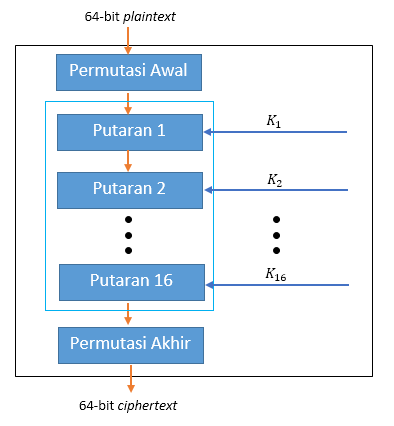
\includegraphics[scale=0.8]{Gambar/proses_enkripsi_des}
	\centering
	\caption{Proses Enkripsi}\label{fig:prosesenkripsi}
\end{figure}

\subsection{Permutasi Awal}\label{subsec:permutasiawal}

Permutasi awal dalam DES menggunakan matriks permutasi \begin{math}mp\end{math}. Masukan dari matriks permutasi \begin{math}mp\end{math} adalah \textit{plaintext}. Tabel \ref{table:awal} menunjukkan matriks permutasi \begin{math}mp\end{math}.

\begin{table}[H]
	\centering
	\caption{Matriks Permutasi Awal}\label{table:awal}
	\begin{tabular}{|l|l|l|l|l|l|l|l|}
			\hline
			58	&	50	&	42	&	34	&	26	&	18	&	10	&	2	\\ \hline
			60	&	52	&	44	&	36	&	28	&	20	&	12	&	4	\\ \hline
			62	&	54	&	46	&	38	&	30	&	22	&	14	&	6	\\ \hline
			64	&	56	&	48	&	40	&	32	&	24	&	16	&	8	\\ \hline
			57	&	49	&	41	&	33	&	25	&	17	&	9	&	1	\\ \hline
			59	&	51	&	43	&	35	&	27	&	19	&	11	&	3	\\ \hline
			61	&	53	&	45	&	37	&	29	&	21	&	13	&	5	\\ \hline
			63	&	55	&	47	&	39	&	31	&	23	&	15	&	7	\\ \hline
	\end{tabular}
\end{table}

Cara kerja dari proses permutasi adalah sebagai berikut. Angka yang ditunjukkan pada posisi ke-\begin{math}i\end{math} matriks \begin{math}mp\end{math} merupakan posisi \textit{bit} dari masukan, sedangkan \begin{math}i\end{math} menunjukkan posisi \textit{bit} dari keluaran. Proses permutasi ditunjukkan oleh persamaan \ref{eq:permutasi}.

\begin{equation}
	keluaran_i = masukan_{p_i}
	\label{eq:permutasi}
\end{equation}

Sebagai contoh, posisi ke-1 dari matriks \begin{math}mp\end{math} menunjukkan angka 58. Maka, \textit{bit} ke-58 dari masukan akan menjadi \textit{bit} ke-1 dari keluaran. Contoh lainnya, posisi ke-62 dari matriks $mp$ menunjukkan angka 23. Maka, \textit{bit} ke-23 dari masukan akan menjadi \textit{bit} ke-62 dari keluaran.

\subsection{Pembangunan Kunci Putaran}

DES menggunakan kunci dengan panjang 64-\textit{bit}. Kunci ini perlu diubah menjadi kunci untuk setiap putaran DES dengan panjang masing-masing 48-\textit{bit}. Proses pembangunan kunci putaran terdiri dari \textit{parity drop}, \textit{shift left}, dan permutasi \textit{P-box}. Gambar \ref{fig:keygenerate} menunjukkan keseluruhan proses dari pembangunan kunci putaran. Pada bagian ini akan dijelaskan masing-masing proses dari pembangunan kunci putaran.

%diagram
\begin{figure}[h]
	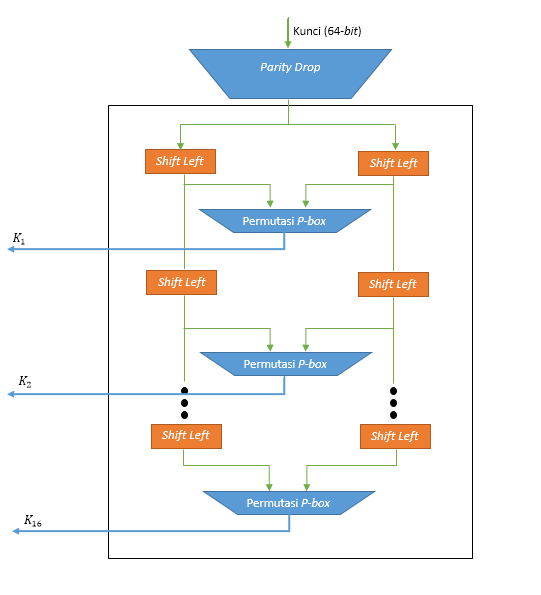
\includegraphics[scale=0.7]{Gambar/key_generate}
	\centering
	\caption{Proses Pembangunan Kunci Putaran}\label{fig:keygenerate}
\end{figure}

\subsubsection{\textit{Parity Drop}}

Pada proses ini, \textit{parity bit} akan dihilangkan dari kunci masukan. \textit{Bit} yang dihilangkan adalah \textit{bit} posisi kelipatan 8, yaitu posisi ke-8, posisi ke-16, posisi ke-24, dan seterusnya sampai posisi ke-64. Proses penghilangan \textit{parity bit} ini menggunakan matriks permutasi \begin{math}p\end{math} seperti ditunjukkan pada Tabel \ref{table:parity_drop}. Cara kerja proses permutasi sama dengan cara kerja proses permutasi pada tahap permutasi awal (Subbab \ref{subsec:permutasiawal}).

\begin{table}[H]
	\begin{center}
		\caption{Matriks Permutasi untuk \textit{Parity Drop}}\label{table:parity_drop}
		\begin{tabular}{|l|l|l|l|l|l|l|l|}
				\hline
				57	&	49	&	41	&	33	&	25	&	17	&	9		&	1		\\ \hline
				58	&	50	&	42	&	34	&	26	&	18	&	10	&	2		\\ \hline
				59	&	51	&	43	&	35	&	27	&	19	&	11	&	3		\\ \hline
				60	&	52	&	44	&	36	&	63	&	55	&	47	&	39	\\ \hline
				31	&	23	&	15	&	7		&	62	&	54	&	46	&	38	\\ \hline
				30	&	22	&	14	&	6		&	61	&	53	&	45	&	37	\\ \hline
				29	&	21	&	13	&	5		&	28	&	20	&	12	&	4		\\ \hline
		\end{tabular}
	\end{center}
\end{table}

Hasil akhir dari proses ini kunci dengan panjang 56-bit.

\subsubsection{\textit{Shift Left}}

Pada proses ini, kunci hasil proses \textit{parity drop} dibagi menjadi 2 bagian dengan panjang masing-masing 28-\textit{bit}, yaitu bagian kiri (\textit{L}) dan bagian kanan (\textit{R}). \begin{math}L\end{math} dan \begin{math}R\end{math} akan digeser ke arah kiri secara sirkular sebanyak 1 atau 2 \textit{bit} tergantung dari urutan putaran. Ketentuan banyak \textit{bit} yang digeser adalah sebagai berikut.

\begin{itemize}
	\item Untuk putaran ke-1, 2, 9, dan 16 maka \begin{math}L\end{math} dan \begin{math}R\end{math} akan digeser ke arah kiri secara sirkular sebanyak 1 \textit{bit}.
	\item Untuk putaran ke-3, 4, 5, 6, 7, 8, 10, 11, 12, 13, 14, dan 15, \begin{math}L\end{math} dan \begin{math}R\end{math} akan digeser ke arah kiri secara sirkular sebanyak 2 \textit{bit}.
\end{itemize}

Sebagai contoh, misalkan \begin{math}L\end{math} dan \begin{math}R\end{math} pada persamaan \ref{eq:L} dan \ref{eq:R}.

\begin{equation}
	L = 1001\: 1010\: 1000\: 0110\: 0110\: 1111\: 1101
	\label{eq:L}
\end{equation}

\begin{equation}
	R = 0001\: 0100\: 0111\: 1110\: 1010\: 0101\: 1011
	\label{eq:R}
\end{equation}

Untuk putaran ke-1, 2, 9, dan 16 maka hasil dari \begin{math}L\end{math} dan \begin{math}R\end{math} akan seperti yang ditunjukkan pada persamaan \ref{eq:L1} dan \ref{eq:R1}.

\begin{equation}
	L = 0011\: 0101\: 0000\: 1100\: 1101\: 1111\: 1011
	\label{eq:L1}
\end{equation}

\begin{equation}
	R = 0010\: 1000\: 1111\: 1101\: 0100\: 1011\: 0110
	\label{eq:R1}
\end{equation}

Sementara itu, jika untuk putaran ke-3, 4, 5, 6, 7, 8, 10, 11, 12, 13, 14, dan 15 akan seperti yang ditunjukkan pada persamaan \ref{eq:L2} dan \ref{eq:R2}.

\begin{equation}
	L = 0110\: 1010\: 0001\: 1001\: 1011\: 1111\: 0110
	\label{eq:L2}
\end{equation}

\begin{equation}
	R = 0101\: 0001\: 1111\: 1010\: 1001\: 0110\: 1100
	\label{eq:R2}
\end{equation}

Kemudian, \begin{math}L\end{math} dan \begin{math}R\end{math} akan disatukan kembali sehingga panjangnya menjadi 56-\textit{bit}.

\subsubsection{Permutasi \textit{P-box}}

Tahap ini adalah proses permutasi untuk mengubah kunci dari proses \textit{Shift Left} dengan panjang 56-\textit{bit} menjadi kunci putaran dengan panjang 48-\textit{bit}. Tabel \ref{table:kompresi_p} menunjukkan matriks permutasi\textit{ P-box} yang digunakan untuk proses ini.

\begin{table}[H]
	\begin{center}
		\caption{Matriks kompresi \textit{P-box}}\label{table:kompresi_p}
		\begin{tabular}{|l|l|l|l|l|l|l|l|}
				\hline
				14	&	17	&	11	&	24	&	1	&	5	&	3	&	28	\\ \hline
				15	&	6	&	21	&	10	&	23	&	19	&	12	&	4	\\ \hline
				26	&	8	&	16	&	7	&	27	&	20	&	13	&	2	\\ \hline
				41	&	52	&	31	&	37	&	47	&	55	&	30	&	40	\\ \hline
				51	&	45	&	33	&	48	&	44	&	49	&	39	&	56	\\ \hline
				32	&	29	&	36	&	50	&	42	&	46	&	53	&	34	\\ \hline
		\end{tabular}
	\end{center}
\end{table}

Hasil keluaran dari proses ini adalah kunci putaran dengan panjang 48-\textit{bit} dan siap dipakai untuk masing-masing putaran.

\subsection{Putaran}

DES terdiri dari 16 putaran. Setiap putaran adalah jaringan Feistel yang akan dijelaskan pada bagian selanjutnya. Gambar \ref{fig:putarandes} menunjukkan ilustrasi dari 16 putaran dari DES.

\begin{figure}[H]
	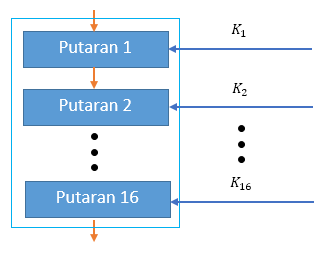
\includegraphics[scale=0.8]{Gambar/putaran_des}
	\centering
	\caption{Putaran dalam DES}\label{fig:putarandes}
\end{figure}

\subsubsection{Jaringan Feistel}

Pada bagian ini akan dijelaskan mengenai sejarah singkat dari jaringan Feistel dan pembahasan jaringan Fesitel.

\subsubsection{Sejarah Singkat}

Jaringan Feistel diciptakan oleh ilmuwan asal Jerman bernama Horst Feistel. Horst Feistel mempublikasikan jaringan ini pada tahun 1973. Jaringan Feistel banyak digunakan dalam berbagai skema enkripsi khususnya digunakan dalam DES.

\subsubsection{Pembahasan}

Masukan dari jaringan Feistel adalah \textit{plaintext} dengan panjang 64-\textit{bit} dan keluaran dari jaringan Feistel adalah \textit{ciphertext} dengan panjang 64-\textit{bit}. Jaringan Feistel menggunakan kunci \begin{math}K\end{math} dan fungsi enkripsi \begin{math}f\end{math} dalam pemrosesan \textit{plaintext}. Selanjutnya akan dijelaskan langkah-langkah pemrosesan \textit{plaintext} pada jaringan Feistel.

\begin{enumerate}
	\item \textit{Plaintext} dibagi menjadi 2 bagian sama panjang, yaitu bagian kiri (\begin{math}L_{i-1}\end{math}) dan bagian kanan (\begin{math}R_{i-1}\end{math}). Huruf \begin{math}i\end{math} menunjukkan urutan dari putaran. Panjang masing-masing bagian adalah 32-\textit{bit}.
	\item Bagian kanan (\begin{math}R_{i-1}\end{math}) pada \textit{plaintext} akan menjadi bagian kiri (\begin{math}L_i\end{math}) dari \textit{ciphertext}. Persamaan \ref{eq:swap} menunjukkan langkah yang sudah dijelaskan.
	\begin{equation}
		L_i = R_{i-1}
		\label{eq:swap}
	\end{equation}
	\item Untuk memperoleh bagian kanan dari \textit{ciphertext} (\begin{math}R_i\end{math}), bagian kanan dari \textit{plaintext} (\begin{math}R_{i-1}\end{math}) dan kunci putaran \begin{math}K_i\end{math} dipetakan dengan fungsi \begin{math}f\end{math}. Kemudian, hasil pemetaan dengan fungsi \begin{math}f\end{math} akan di \textit{exclusive-or} (XOR) dengan bagian kiri dari plaintext (\begin{math}L_{i-1}\end{math}). Persamaan \ref{eq:xor} menunjukkan langkah yang sudah dijelaskan.
	\begin{equation}
		R_i = L_{i-1} \oplus f(R_{i-1}, K_i)
		\label{eq:xor}
	\end{equation}
	\item Hasil akhirnya berupa \textit{ciphertext} dengan 2 bagian sama panjang, yaitu bagian kiri (\begin{math}L_i\end{math}) dan bagian kanan (\begin{math}R_i\end{math}). 
\end{enumerate}

Gambar \ref{fig:jaringanfeistel} menunjukkan ilustrasi dari langkah-langkah yang sudah dijelaskan.

%diagram
\begin{figure}[H]
	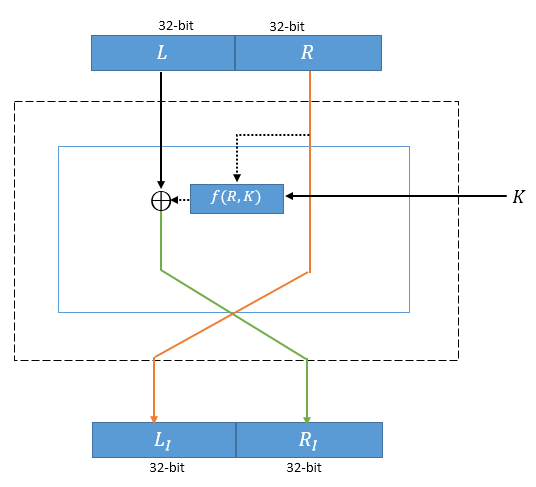
\includegraphics[scale=0.6]{Gambar/jaringan_feistel}
	\centering
	\caption{Jaringan Feistel}\label{fig:jaringanfeistel}
\end{figure}

\subsubsection{Fungsi DES}

Fungsi DES adalah fungsi \begin{math}f\end{math} yang digunakan dalam jaringan Feistel pada Gambar \ref{fig:jaringanfeistel}. Fungsi DES terdiri dari 4 bagian, yaitu ekspansi \textit{P-box}, operasi XOR, substitusi \textit{S-box}, dan permutasi. Pada bagian selanjutnya akan dijelaskan masing-masing bagian dari fungsi DES.

\subsubsection{Ekspansi \textit{P-box}}

Pada bagian ini, masukan berupa blok bagian kanan dari \textit{plaintext} (\begin{math}R\end{math}) dengan panjang 32-\textit{bit}. Ekspansi \textit{P-box} menggunakan matriks permutasi \begin{math}p\end{math} yang ditunjukkan pada tabel \ref{table:Pbox}.

\begin{table}[H]
	\begin{center}
		\caption{\textit{P-box}}\label{table:Pbox}
		\begin{tabular}{|l|l|l|l|l|l|}
				\hline
				32 	& 1		& 2 	& 3 	& 4 	& 5		\\ \hline
				4 	& 5		& 6 	& 7 	& 8 	& 9		\\ \hline
				8 	& 9		& 10 	& 11 	& 12 	& 13	\\ \hline
				12 	& 13	& 14 	& 15 	& 16 	& 17	\\ \hline
				16 	& 17	& 18 	& 19 	& 20 	& 21	\\ \hline
				20 	& 21	& 22 	& 23 	& 24 	& 25	\\ \hline
				24 	& 25	& 26 	& 27 	& 28 	& 29	\\ \hline
				28 	& 29	& 30 	& 31 	& 32 	& 1		\\ \hline
		\end{tabular}
	\end{center}
\end{table}

Hasil keluaran dari ekspansi \textit{P-box} adalah blok dengan panjang 48-\textit{bit}.

\subsubsection{Operasi XOR}
Setelah ekspansi \textit{P-box}, dilakukan operasi XOR antara \begin{math}R\end{math} dengan kunci putaran ke-\begin{math}i\end{math}, \begin{math}K_i\end{math}. Kunci putaran hanya digunakan pada bagian ini saja.

\subsubsection{Substitusi \textit{S-box}}

Pada bagian ini, akan dilakukan substitusi pada \begin{math}R\end{math} dengan menggunakan \textit{S-box}. Masukan dari \textit{S-box} adalah \begin{math}R\end{math} dengan panjang 48-\textit{bit} dan keluarannya adalah \begin{math}R\end{math} dengan panjang 32-\textit{bit}. \begin{math}R\end{math} akan dibagi menjadi 8 blok dengan panjang masing-masing 6-\textit{bit}. Setiap blok memiliki \textit{S-box} masing-masing. Blok pertama menggunakan \textit{S-box} pertama, blok kedua menggunakan \textit{S-box} kedua, dan seterusnya. Berikut masing-masing dari \textit{S-box} ditunjukkan pada Tabel \ref{table:s_box1} sampai Tabel \ref{table:s_box8}.

\begin{table}[H]
	\caption{\textit{S-box} 1}\label{table:s_box1}
	\begin{center}
		\begin{tabular}{|l|l|l|l|l|l|l|l|l|l|l|l|l|l|l|l|l|}
				\hline
				& 0 & 1	& 2 & 3 & 4 & 5 & 6 & 7 & 8 & 9 & 10 & 11 & 12 & 13 & 14 & 15	\\ \hline
			0 & 14 & 4 & 13 & 1 & 2 & 15 & 11 & 8 & 3 & 10 & 6 & 12 & 5 & 9 & 0 & 7	\\ \hline
			1 & 0 & 15 & 7 & 4 & 14 & 2 & 13 & 10 & 3 & 6 & 12 & 11 & 9 & 5 & 3 & 8	\\ \hline
			2 & 4 & 1 & 14 & 8 & 13 & 6 & 2 & 11 & 15 & 12 & 9 & 7 & 3 & 10 & 5 & 0	\\ \hline
			3 & 15 & 12 & 8 & 2 & 4 & 9 & 1 & 7 & 5 & 11 & 3 & 14 & 10 & 0 & 6 & 13	\\ \hline
		\end{tabular}
	\end{center}
\end{table}

\begin{table}[H]
	\caption{\textit{S-box} 2}\label{table:s_box2}
	\begin{center}
		\begin{tabular}{|l|l|l|l|l|l|l|l|l|l|l|l|l|l|l|l|l|}
				\hline
				& 0 & 1	& 2 & 3 & 4 & 5 & 6 & 7 & 8 & 9 & 10 & 11 & 12 & 13 & 14 & 15	\\ \hline
			0 & 15 & 1 & 8 & 14 & 6 & 11 & 3 & 4 & 9 & 7 & 2 & 13 & 12 & 0 & 5 & 10	\\ \hline
			1 & 3 & 13 & 4 & 7 & 15 & 2 & 8 & 12 & 12 & 0 & 1 & 10 & 6 & 9 & 11 & 5	\\ \hline
			2 & 0 & 14 & 7 & 11 & 10 & 4 & 13 & 1 & 5 & 8 & 12 & 6 & 9 & 3 & 2 & 15	\\ \hline
			3 & 13 & 8 & 10 & 1 & 3 & 15 & 4 & 2 & 11 & 6 & 7 & 12 & 0 & 5 & 14 & 9	\\ \hline
		\end{tabular}
	\end{center}
\end{table}

\begin{table}[H]
	\caption{\textit{S-box} 3}\label{table:s_box3}
	\begin{center}
		\begin{tabular}{|l|l|l|l|l|l|l|l|l|l|l|l|l|l|l|l|l|}
				\hline
				& 0 & 1	& 2 & 3 & 4 & 5 & 6 & 7 & 8 & 9 & 10 & 11 & 12 & 13 & 14 & 15	\\ \hline
			0 & 10 & 0 & 9 & 14 & 6 & 3 & 15 & 5 & 1 & 13 & 12 & 7 & 11 & 4 & 2 & 8	\\ \hline
			1 & 13 & 7 & 0 & 9 & 3 & 4 & 6 & 10 & 2 & 8 & 5 & 14 & 12 & 11 & 15 & 1	\\ \hline
			2 & 13 & 6 & 4 & 9 & 8 & 15 & 3 & 0 & 11 & 1 & 2 & 12 & 5 & 10 & 14 & 7	\\ \hline
			3 & 1 & 10 & 13 & 0 & 6 & 9 & 8 & 7 & 4 & 15 & 14 & 3 & 11 & 5 & 2 & 12	\\ \hline
		\end{tabular}
	\end{center}
\end{table}

\begin{table}[H]
	\caption{\textit{S-box} 4}\label{table:s_box4}
	\begin{center}
		\begin{tabular}{|l|l|l|l|l|l|l|l|l|l|l|l|l|l|l|l|l|}
				\hline
				& 0 & 1	& 2 & 3 & 4 & 5 & 6 & 7 & 8 & 9 & 10 & 11 & 12 & 13 & 14 & 15	\\ \hline
			0 & 7	&	13	&	14	&	3	&	0	&	6	&	9	&	10	&	1	&	2	&	8	&	5	&	11	&	12	&	4	&	15	\\ \hline
			1 & 13	&	8	&	11	&	5	&	6	&	15	&	0	&	3	&	4	&	7	&	2	&	12	&	1	&	10	&	14	&	9	\\ \hline
			2 & 10	&	6	&	9	&	0	&	12	&	11	&	7	&	13	&	15	&	1	&	3	&	14	&	5	&	2	&	8	&	4	\\ \hline
			3 & 3	&	15	&	0	&	6	&	10	&	1	&	13	&	8	&	9	&	4	&	5	&	11	&	12	&	7	&	2	&	14	\\ \hline
		\end{tabular}
	\end{center}
\end{table}

\begin{table}[H]
	\caption{\textit{S-box} 5}\label{table:s_box5}
	\begin{center}
		\begin{tabular}{|l|l|l|l|l|l|l|l|l|l|l|l|l|l|l|l|l|}
				\hline
				& 0 & 1	& 2 & 3 & 4 & 5 & 6 & 7 & 8 & 9 & 10 & 11 & 12 & 13 & 14 & 15	\\ \hline
			0	&	2	&	12	&	4	&	1	&	7	&	10	&	11	&	6	&	8	&	5	&	3	&	15	&	13	&	0	&	14	&	9	\\ \hline
			1	&	14	&	11	&	2	&	12	&	4	&	7	&	13	&	1	&	5	&	0	&	15	&	10	&	3	&	9	&	8	&	6	\\ \hline
			2	&	4	&	2	&	1	&	11	&	10	&	13	&	7	&	8	&	15	&	9	&	12	&	5	&	6	&	3	&	0	&	14	\\ \hline
			3	&	11	&	8	&	12	&	7	&	1	&	14	&	2	&	13	&	6	&	15	&	0	&	9	&	10	&	4	&	5	&	3	\\ \hline
		\end{tabular}
	\end{center}
\end{table}

\begin{table}[H]
	\caption{\textit{S-box} 6}\label{table:s_box6}
	\begin{center}
		\begin{tabular}{|l|l|l|l|l|l|l|l|l|l|l|l|l|l|l|l|l|}
				\hline
				& 0 & 1	& 2 & 3 & 4 & 5 & 6 & 7 & 8 & 9 & 10 & 11 & 12 & 13 & 14 & 15	\\ \hline
			0	&	12	&	1	&	10	&	15	&	9	&	2	&	6	&	8	&	0	&	13	&	3	&	4	&	14	&	7	&	5	&	11	\\ \hline
			1	&	10	&	15	&	4	&	2	&	7	&	12	&	9	&	5	&	6	&	1	&	13	&	14	&	0	&	11	&	3	&	8	\\ \hline
			2	&	9	&	14	&	15	&	5	&	2	&	8	&	12	&	3	&	7	&	0	&	4	&	10	&	1	&	13	&	11	&	6	\\ \hline
			3	&	4	&	3	&	2	&	12	&	9	&	5	&	15	&	10	&	11	&	14	&	1	&	7	&	6	&	0	&	8	&	13	\\ \hline
		\end{tabular}
	\end{center}
\end{table}

\begin{table}[H]
	\caption{\textit{S-box} 7}\label{table:s_box7}
	\begin{center}
		\begin{tabular}{|l|l|l|l|l|l|l|l|l|l|l|l|l|l|l|l|l|}
				\hline
					& 0 & 1	& 2 & 3 & 4 & 5 & 6 & 7 & 8 & 9 & 10 & 11 & 12 & 13 & 14 & 15	\\ \hline
				0	&	4	&	11	&	2	&	14	&	15	&	0	&	8	&	13	&	3	&	12	&	9	&	7	&	5	&	10	&	6	&	1	\\ \hline
				1	&	13	&	0	&	11	&	7	&	4	&	9	&	1	&	10	&	14	&	3	&	5	&	12	&	2	&	15	&	8	&	6	\\ \hline
				2	&	1	&	4	&	11	&	13	&	12	&	3	&	7	&	14	&	10	&	15	&	6	&	8	&	0	&	5	&	9	&	2	\\ \hline
				3	&	6	&	11	&	13	&	8	&	1	&	4	&	10	&	7	&	9	&	5	&	0	&	15	&	14	&	2	&	3	&	12	\\ \hline
		\end{tabular}
	\end{center}
\end{table}

\begin{table}[H]
	\caption{\textit{S-box} 8}\label{table:s_box8}
	\begin{center}
		\begin{tabular}{|l|l|l|l|l|l|l|l|l|l|l|l|l|l|l|l|l|}
				\hline
				& 0 & 1	& 2 & 3 & 4 & 5 & 6 & 7 & 8 & 9 & 10 & 11 & 12 & 13 & 14 & 15	\\ \hline
			0	&	13	&	2	&	8	&	4	&	6	&	15	&	11	&	1	&	10	&	9	&	3	&	14	&	5	&	0	&	12	&	7	\\ \hline
			1	&	1	&	15	&	13	&	8	&	10	&	3	&	7	&	4	&	12	&	5	&	6	&	11	&	0	&	14	&	9	&	2	\\ \hline
			2	&	7	&	11	&	4	&	1	&	9	&	12	&	14	&	2	&	0	&	6	&	10	&	13	&	15	&	3	&	5	&	8	\\ \hline
			3	&	2	&	1	&	14	&	7	&	4	&	10	&	8	&	13	&	15	&	12	&	9	&	0	&	3	&	5	&	6	&	11	\\ \hline
		\end{tabular}
	\end{center}
\end{table}

Proses subsitusi terjadi sebagai berikut. Kombinasi \textit{bit} ke-1 dan \textit{bit} ke-6 pada blok akan menunjukkan posisi baris pada \textit{S-box}. Kemudian, kombinasi dari \textit{bit} ke-2 sampai ke-5 menunjukkan posisi kolom pada \textit{S-box}. Setelah itu, angka yang ditunjuk oleh baris dan kolom pada \textit{S-box} ini akan menjadi blok keluaran.

Sebagai contoh, misalkan masukan dari \textit{S-box} pertama adalah 110011. Maka, kombinasi \textit{bit}nya adalah 11 untuk baris dan 1001 untuk kolom. Jadi, baris yang dipilih adalah baris ke-3 dan kolom yang dipilih adalah kolom ke-9. Angka yang ditunjuk oleh \textit{S-box} pertama pada baris ke-3 dan kolom ke-9 adalah 11. Maka, blok keluaran untuk \textit{S-box} pertama adalah 1011. Lalu, setelah seluruh blok masukan diproses dengan \textit{S-box} masing-masing, seluruh blok keluaran digabungkan menjadi blok dengan panjang 32-\textit{bit}.

\subsubsection{Permutasi}

Bagian ini adalah bagian terakhir dari fungsi DES. Masukan dari bagian ini adalah blok keluaran dari proses subsitusi \textit{S-box}, yaitu blok dengan panjang 32-\textit{bit}. Proses permutasi dilakukan dengan menggunakan matriks \begin{math}m\end{math} yang ditunjukkan oleh Tabel \ref{table:permutasi_langsung}. Hasil keluaran dari bagian ini adalah blok dengan panjang 32-\textit{bit}.

\begin{table}[H]
	\begin{center}
		\caption{Matriks Permutasi \textit{m}}\label{table:permutasi_langsung}
		\begin{tabular}{|l|l|l|l|l|l|l|l|}
				\hline
				16	&	7	&	20	&	21	&	29	&	12	&	28	&	17	\\ \hline
				1	&	15	&	23	&	26	&	5	&	18	&	31	&	10		\\ \hline
				2	&	8	&	24	&	14	&	32	&	27	&	3	&	9				\\ \hline
				19	&	13	&	30	&	6	&	22	&	11	&	4	&	25	\\ \hline
		\end{tabular}
	\end{center}
\end{table}

Setelah proses permutasi ini, hasil dari proses permutasi akan di exclusive-or (XOR) dengan \begin{math}L_{i-1}\end{math} seperti yang sudah dijelaskan pada bagian Jaringan Feistel. Hasil XOR adalah bagian kanan dari ciphertext (\begin{math}R_i\end{math}). Setelah itu, \begin{math}L_i\end{math} dan \begin{math}R_i\end{math} akan digabungkan kemudian dijadikan sebagai masukan untuk putaran selanjutnya.

\subsection{Permutasi Akhir}

Setelah dilakukan 16 putaran, tahap terakhir dari enkripsi DES adalah permutasi akhir. Proses permutasi akhir menggunakan matriks yang ditunjukkan pada Tabel \ref{table:akhir}. Hasil dari proses permutasi akhir adalah 64-bit \textit{ciphertext}.

\begin{table}[H]
	\centering
	\caption{Matriks Permutasi Akhir}\label{table:akhir}
	\begin{tabular}{|l|l|l|l|l|l|l|l|}
			\hline
			40	&	8	&	48	&	16	&	56	&	24	&	64	&	32	\\ \hline
			39	&	7	&	47	&	15	&	55	&	23	&	63	&	31	\\ \hline
			38	&	6	&	46	&	14	&	54	&	22	&	62	&	30	\\ \hline
			37	&	5	&	45	&	13	&	53	&	21	&	61	&	29	\\ \hline
			36	&	4	&	44	&	12	&	52	&	20	&	60	&	28	\\ \hline
			35	&	3	&	43	&	11	&	51	&	19	&	59	&	27	\\ \hline
			34	&	2	&	42	&	10	&	50	&	18	&	58	&	26	\\ \hline
			33	&	1	&	41	&	9	&	49	&	17	&	57	&	25	\\ \hline
	\end{tabular}
\end{table}

\section{Fungsi \textit{Hash}}\label{sec:fungsihash}

Fungsi \textit{hash} adalah fungsi yang memiliki masukan berupa \textit{string} dengan panjang sembarang dan menghasilkan keluaran berupa \textit{string} dengan panjang yang tetap. Masukan dari fungsi \textit{hash} dinamakan \textit{message}. Hasil keluaran dari fungsi \textit{hash} dinamakan \textit{digest}. \textit{Message} \begin{math}m\end{math} akan dipetakan dengan fungsi \textit{hash} \begin{math}H\end{math} menghasilkan \textit{digest} \begin{math}h\end{math}. Persamaan \ref{eq:fungsihash} menunjukkan pemetaan \begin{math}m\end{math} dengan \begin{math}H\end{math} yang menghasilkan \begin{math}h\end{math}.

\begin{equation}
	h = H(m) \label{eq:fungsihash}
\end{equation}

Fungsi \textit{hash} harus memiliki 3 kriteria sebagai berikut\cite{forouzan2007cryptography}.

\begin{enumerate}
	\item Preimage Resistance \\
	Untuk setiap \begin{math}h=H(m)\end{math} yang dihasilkan, tidak mungkin dikembalikan \begin{math}m\end{math} sedemikian rupa sehingga \begin{math}H(m)=h\end{math}. Dalam proses pembuatan \textit{digest}, fungsi \textit{hash} menghilangkan beberapa bagian dari \begin{math}m\end{math} (\textit{lossy}). Maka dari itu, \textit{digest} tidak bisa dikembalikan menjadi \textit{message}. Itulah sebabnya fungsi \textit{hash} disebut fungsi satu arah.
	\item Second Preimage Resistance \\
	Untuk setiap \begin{math}m\end{math} yang diberikan, tidak mungkin mencari \begin{math}m' \neq m\end{math} sedemikian rupa sehingga \begin{math}H(m') = H(m)\end{math}.
	\item Collision Resistance \\
	Tidak mungkin mencari pasangan \begin{math}m\end{math} dan \begin{math}m'\end{math} sedemikian rupa sehingga \begin{math}h=H(m)\end{math} sama dengan \begin{math}h'=h(m')\end{math}. Untuk 2 \textit{message} yang berbeda tidak mungkin menghasilkan \textit{digest} yang sama.
\end{enumerate}

Contoh fungsi \textit{hash} antara lain MD-2, MD-4, MD-5, SHA-0, SHA-1, SHA-256, dan SHA-512.

\section{\textit{Secure Hashing Algorithm} 512 (SHA-512)}\label{sec:SHA512}

\textit{Secure hashing algorithm} 512 atau SHA-512 adalah algoritma fungsi \textit{hash} yang menghasilkan \textit{digest} dengan panjang 512-\textit{bit}. Proses dari SHA-512 terdiri dari \textit{message padding}, inisialisasi konstanta awal, ekspansi blok \textit{message}, fungsi kompresi, dan putaran. Bagian selanjutnya akan menjelaskan masing-masing proses dari SHA-512.

\subsection{\textit{Message Padding}}

Sebelum \textit{digest} dibuat, \textit{message} akan di\textit{padding} terlebih dahulu. Pertama-tama, blok \textit{message} \begin{math}M\end{math} akan dipadding dengan blok \begin{math}L\end{math}. Blok \begin{math}L\end{math} berisi informasi mengenai panjang dari \begin{math}M\end{math}. Panjang dari blok L adalah 128-\textit{bit}. Kemudian, gabungan dari blok \begin{math}M\end{math} dan \begin{math}L\end{math} akan di\textit{padding} lagi dengan blok \textit{padding} \begin{math}P\end{math} sampai panjang dari gabungan blok \begin{math}M, L\end{math}, dan \begin{math}P\end{math} mencapai kelipatan 1024-\textit{bit}. Panjang dari blok \textit{padding} \begin{math}P\end{math} bervariasi. Persamaan \ref{eq:blokp1} menunjukkan rumus untuk menghitung panjang dari blok \textit{padding} \begin{math}P\end{math}.

\begin{equation}
	(M + P + 128) = 0\: mod\: 1024 \qquad\Rightarrow\qquad P = (-M - 128)\: mod\: 1024 \label{eq:blokp1}
\end{equation}

Isi dari blok \textit{padding} \begin{math}P\end{math} adalah angka 1 diikuti dengan angka 0. Sebagai contoh, jika panjang dari \textit{message} (\begin{math}M\end{math}) adalah 2590 \textit{bit}, maka panjang dari blok \textit{padding} \begin{math}P\end{math} ditunjukkan pada persamaan \ref{eq:blokp2}.

\begin{gather}
	P = (-2590 - 128)\: mod\: 1024 \nonumber \\
		= -2718\: mod\: 1024 \label{eq:blokp2} \\
		= 354 \nonumber
\end{gather}

Maka, dari persamaan \ref{eq:blokp2}, panjang dari blok \begin{math}P\end{math} adalah 354 \textit{bit}. Isi dari blok \begin{math}P\end{math} adalah 1 \textit{bit} angka 1 diikuti dengan 353 \textit{bit} angka 0.

\subsection{Inisialisasi Konstanta Awal}

Setelah proses \textit{message padding}, proses selanjutnya adalah inisialisasi konstanta awal. Ada 8 konstanta awal yang akan dibentuk. Delapan konstanta awal ini akan diberi nama \begin{math}A_0, B_0, C_0, \end{math} \begin{math}D_0, E_0, F_0, G_0,\end{math} dan \begin{math}H_0\end{math}. Panjang masing-masing konstanta awal ini adalah 64-\textit{bit}. Setiap nilai konstanta awal diperoleh dari nilai di belakang koma dari akar kuadrat bilangan prima. Kemudian, nilai di belakang koma ini akan diubah menjadi heksadesimal. Bilangan prima yang digunakan untuk masing-masing konstanta awal adalah bilangan prima awal secara berurutan, yaitu 2, 3, 5, 7, 11, 13, 17, dan 19.

Sebagai contoh, misalkan akan dicari nilai untuk \begin{math}A_0\end{math}. \begin{math}A_0\end{math} merupakan konstanta awal pertama maka bilangan prima yang digunakan adalah bilangan prima urutan pertama, yaitu 2. Setelah itu, akan dihitung akar kuadrat dari 2. Kemudian, angka di belakang koma dari akar kuadrat 2 akan diubah menjadi heksadesimal. Nilai heksadesimal inilah yang menjadi nilai dari \begin{math}A_0\end{math}. Persamaan \ref{eq:ubahkonstantaawal} menunjukkan langkah yang sudah dijelaskan.

\begin{gather}
	A_0 = \sqrt{2} \nonumber \\
	= 1.4142135623730950 \nonumber \\
	= (1.6A09E667F3BCC908)_{16} \label{eq:ubahkonstantaawal} \\
	= 6A09E667F3BCC908 \nonumber
\end{gather}

Tabel \ref{table:konstantaawal} menunjukkan nilai masing-masing konstanta.

\begin{table}[H]
	\centering
	\caption{Konstanta Awal}\label{table:konstantaawal}
	\begin{tabular}{| >{$}l<{$} | >{$}l<{$} | >{$}l<{$} | >{$}l<{$} |}
			\hline
			Konstanta	&	Nilai							&	Konstanta &	Nilai							\\ \hline
			A_0				&	6A09E667F3BCC908	&	E_0				&	510E527FADE682D1	\\ \hline
			B_0				&	BB67AE8584CAA73B	&	F_0				&	9B05688C2B3E6C1F	\\ \hline
			C_0				&	3C6EF372FE94F828	&	G_0				&	1F83D9ABFB41BD6B	\\ \hline
			D_0				&	A54FF53A5F1D36F1	&	H_0				&	5BE0CD19137E2179	\\ \hline
	\end{tabular}
\end{table}

\subsection{Ekspansi Blok Message}\label{subsec:expansiblokmsg}

Setelah inisialisasi konstanta awal, proses berikutnya adalah ekspansi blok \textit{message}. Sesudah blok \textit{message} di\textit{padding}, blok \textit{message} akan dibagi menjadi beberapa blok yang panjangnya masing-masing 1024-\textit{bit}. Kemudian, setelah dibagi menjadi beberapa blok 1024-\textit{bit}, masing-masing dari 1024-\textit{bit} akan dibagi lagi menjadi blok-blok dengan panjang 64-\textit{bit}. Blok dengan panjang 64-\textit{bit} ini dinamakan \textit{word}.

Satu blok 1024-\textit{bit} terdiri dari 16 \textit{word}. Proses ekspansi blok \textit{message} akan mengekspansi dari 16 \textit{word} dari 1 blok 1024-\textit{bit} menjadi 80 \textit{word}. Masing-masing \textit{word} ini akan diberi nama \begin{math}W_0\end{math} sampai \begin{math}W_{79}\end{math}. Untuk \begin{math}W_0\end{math} sampai \begin{math}W_{15}\end{math} berisi dari 16 \textit{word} pertama dari blok 1024-\textit{bit}. Sementara itu, \begin{math}W_{16}\end{math} sampai \begin{math}W_{79}\end{math} diperoleh dengan rumus dasar yang ditunjukkan oleh persamaan \ref{eq:ekspansiword1}.

\begin{equation}
	W_i = W_{i-16} \oplus RotShift_{1-8-7}(W_{i-15}) \oplus W_{i-7} \oplus RotShift_{19-61-6}(W_{i-2}) \label{eq:ekspansiword1}
\end{equation}

Sebagai contoh untuk memperoleh nilai dari \begin{math}W_{60}\end{math}, maka rumus dasarnya adalah seperti yang ditunjukkan pada persamaan \ref{eq:ekspansiword2}.

\begin{equation}
	W_{60} = W_{44} \oplus RotShift_{1-8-7}(W_{45}) \oplus W_{53} \oplus RotShift_{19-61-6}(W_{58}) \label{eq:ekspansiword2}
\end{equation}

\textit{RotShift} pada persamaan \ref{eq:ekspansiword1} dan \ref{eq:ekspansiword2} adalah hasil \textit{exclusive-or} (XOR) dari operasi rotasi ke kanan dan \textit{shift left}. Rumus untuk rotasi ke kanan dan \textit{shift left} ditunjukkan pada persamaan \ref{eq:ekspansiword3}.

\begin{equation}
	RotShift_{l-m-n}(x) = RotR_l(x) \oplus RotR_m(x) \oplus ShL_n(x) \label{eq:ekspansiword3}
\end{equation}

\begin{math}RotR_i(x)\end{math} pada persamaan \ref{eq:ekspansiword3} adalah rotasi ke kanan \begin{math}x\end{math} sebanyak \begin{math}i\end{math} \textit{bit}. Sebagai contoh, misalkan \begin{math}i=2\end{math} dan \begin{math}x=1001\end{math}, maka hasil dari \begin{math}RotR_2(1001)\end{math} ditunjukkan pada persamaan \ref{eq:ekspansiword4}.

\begin{align}
	i = 1 \qquad\Rightarrow\qquad x = 1100 \nonumber \\
	i = 2 \qquad\Rightarrow\qquad x = 0110 \label{eq:ekspansiword4} \\
	RotR_2(1001) = 0110 \nonumber
\end{align}

Sementara itu, \begin{math}ShL_i(x)\end{math} pada persamaan \ref{eq:ekspansiword3} adalah operasi \textit{shift left} \begin{math}x\end{math} sebanyak \begin{math}i\end{math} \textit{bit} di\textit{padding} dengan angka 0. Sebagai contoh, misalkan \begin{math}i=2\end{math} dan \begin{math}x=1011\end{math}, maka hasil dari \begin{math}ShL_2(1011)\end{math} ditunjukkan pada persamaan \ref{eq:ekspansiword5}.

\begin{align}
	i = 1 \qquad\Rightarrow\qquad x = 0110 \nonumber \\
	i = 2 \qquad\Rightarrow\qquad x = 1100 \label{eq:ekspansiword5} \\
	ShL_2(1011) = 1100 \nonumber
\end{align}

Setelah ekspansi blok \textit{message} menjadi 80 \textit{word} untuk setiap blok \textit{message}, proses selanjutnya adalah putaran dari SHA-512. Proses putaran SHA-512 akan dijelaskan pada bagian selanjutnya.

\subsection{Fungsi Kompresi dan Putaran}\label{subsec:putaransha}

Fungsi kompresi adalah proses yang mengkompresi blok 512-\textit{bit} dan blok \textit{message} yang berukuran 1024-\textit{bit} menjadi blok keluaran dengan panjang 512-\textit{bit}. Fungsi kompresi ini terdiri dari 80 putaran SHA-512. 

\subsubsection{Struktur Putaran}

Masukan dari putaran SHA-512 adalah blok dengan panjang 512-\textit{bit} terdiri dari 8 \textit{word} (\textit{A, B, C, D, E, F, G,} dan \textit{H}). Untuk putaran pertama, blok 512-\textit{bit} diperoleh dari konstanta awal (\begin{math}A_0\end{math} sampai \begin{math}H_0\end{math}) sedangkan untuk putaran kedua dan selanjutnya blok 512-\textit{bit} diperoleh dari hasil dari putaran sebelumnya. Gambar \ref{fig:strukturputaran} menunjukkan ilustrasi proses yang sudah dijelaskan.

%diagram
\begin{figure}[H]
	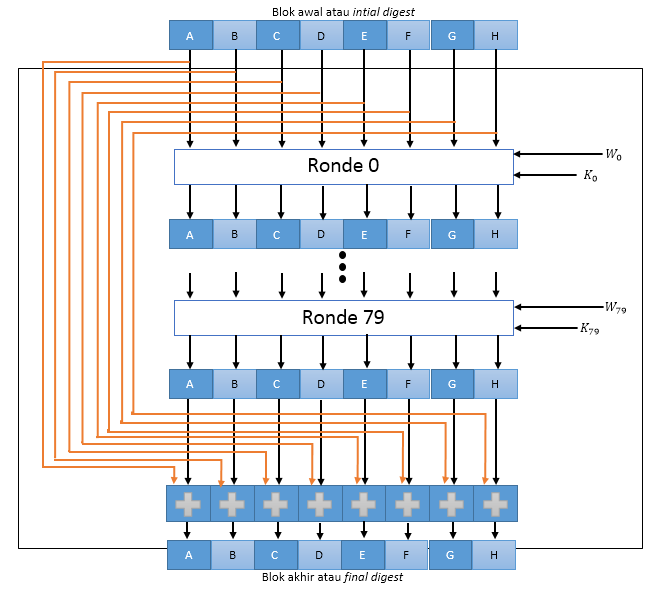
\includegraphics[scale=0.7]{Gambar/compression_function}
	\centering
	\caption{Struktur Putaran dalam SHA-512}\label{fig:strukturputaran}
\end{figure}

Dalam 1 putaran SHA-512, \textit{word} keluaran diperoleh dari salinan word \textit{masukan}, berikut menunjukkan masukan dan keluaran dari masing-masing \textit{word}.

\begin{itemize}
	\item \textit{Word} keluaran \textit{B} diperoleh dari \textit{word} masukan \textit{A}
	\item \textit{Word} keluaran \textit{C} diperoleh dari \textit{word} masukan \textit{B}
	\item \textit{Word} keluaran \textit{D} diperoleh dari \textit{word} masukan \textit{C}
	\item \textit{Word} keluaran \textit{F} diperoleh dari \textit{word} masukan \textit{E}
	\item \textit{Word} keluaran \textit{G} diperoleh dari \textit{word} masukan \textit{F}
	\item \textit{Word} keluaran \textit{H} diperoleh dari \textit{word} masukan \textit{G}
\end{itemize}

Gambar \ref{fig:masukankeluaranword} menunjukkan ilustrasi dari masukan dan keluaran dalam 1 putaran SHA-512 untuk setiap \textit{word}.

%diagram
\begin{figure}[H]
	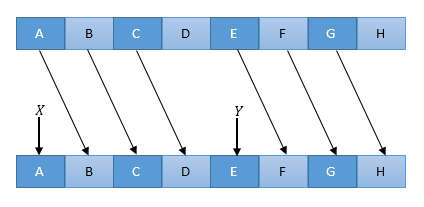
\includegraphics[scale=0.8]{Gambar/sha_round}
	\centering
	\caption{Masukan dan Keluaran dalam 1 Putaran SHA-512}\label{fig:masukankeluaranword}
\end{figure}

Untuk nilai \textit{word} keluaran \textit{A} dan \textit{E} diperoleh dari \textit{word} \textit{X} dan \textit{Y}. \textit{Word} \textit{X} dan \textit{Y} ini diperoleh dari sebuah fungsi khusus. Gambar \ref{fig:fungsikhusus} menunjukkan struktur dari fungsi khusus. Berikut akan dijelaskan struktur dari fungsi khusus.

\subsubsection{Struktur Fungsi Khusus}

%diagram
\begin{figure}[H]
	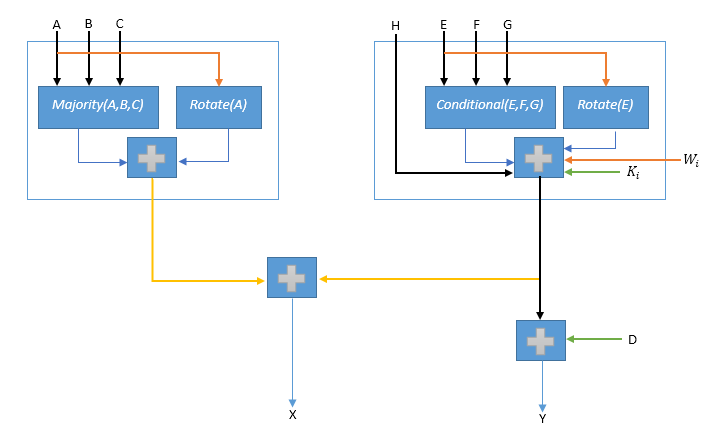
\includegraphics[scale=0.7]{Gambar/complex_function}
	\centering
	\caption{Fungsi Khusus dalam 1 Putaran SHA-512}\label{fig:fungsikhusus}
\end{figure}

\textit{Word Y} pada gambar \ref{fig:fungsikhusus} diperoleh dari proses persamaan \ref{eq:fungsikhusus1}.

\begin{equation}
	Y = D + (Conditional(E,F,G) + Rotate(E) + W_i + K_i + H) \label{eq:fungsikhusus1}
\end{equation}

Nilai \begin{math}W_i\end{math} diperoleh dari proses Ekspansi Blok \textit{Message} (Subbab \ref{subsec:expansiblokmsg}), dimana \textit{i} menunjukkan urutan dari putaran. Nilai \begin{math}K_i\end{math} pada persamaan \ref{eq:fungsikhusus1} diperoleh dari nilai belakang koma akar kubik bilangan prima ke-\begin{math}(i+1)\end{math}. Kemudian, nilai belakang koma ini akan dikonversi menjadi heksadesimal. 

Bilangan prima yang digunakan untuk menghitung nilai \begin{math}K_i\end{math} dimulai dari 2 untuk \begin{math}K_0\end{math}, 3 untuk \begin{math}K_1\end{math}, dan seterusnya secara berurutan sampai 409 untuk \begin{math}K_{79}\end{math}. Persamaan \ref{eq:fungsikhusus2} menunjukkan cara untuk menghitung salah satu dari nilai \begin{math}K_i\end{math}.

\begin{gather}
	K_{79} = \sqrt[3]{409} \nonumber \\
	= 7.4229141204362155 \nonumber \\
	= (7.6C44198C4A475817)_{16} \label{eq:fungsikhusus2} \\
	= 6C44198C4A475817 \nonumber
\end{gather}

Sementara itu, untuk operasi \textit{Conditional} pada persamaan \ref{eq:fungsikhusus1} adalah operasi \textit{AND}, \textit{OR} dan \textit{XOR} dari \textit{bit-bit} setiap \textit{word}. Rumus dari \textit{Conditional} ditunjukkan oleh persamaan \ref{eq:fungsikhusus3}.

\begin{equation}
	Conditional(x,y,z) = (x\: AND\: y) \oplus (NOT\: x\: AND\: z) \label{eq:fungsikhusus3}
\end{equation}

Operasi \textit{Rotate} pada persamaan \ref{eq:fungsikhusus1} adalah hasil \textit{exclusive-or} (XOR) dari \begin{math}RotR_i(x)\end{math}. \begin{math}RotR_i(x)\end{math} merupakan operasi rotasi ke kanan \textit{x} sebanyak \textit{i-bit} yang sudah dijelaskan pada proses Ekspansi Blok Message (Subbab \ref{subsec:expansiblokmsg}). Rumus dari \textit{Rotate} ditunjukkan pada persamaan \ref{eq:fungsikhusus4}.

\begin{equation}
	Rotate(x) = RotR_{28}(x) \oplus RotR_{34}(x) \oplus RotR_{39}(x) \label{eq:fungsikhusus4}
\end{equation}

Hasil pertambahan \textit{bit-bit} operasi \textit{Conditional}, operasi \textit{Rotate}, \begin{math}W_i\end{math}, \begin{math}K_i\end{math}, dan \textit{word} \begin{math}H\end{math} akan ditambahkan dengan \textit{word} \begin{math}D\end{math} untuk menghasilkan \textit{word} \begin{math}Y\end{math}.

Kemudian, \textit{word} \begin{math}X\end{math} pada Gambar \ref{fig:fungsikhusus} diperoleh dari persamaan \ref{eq:fungsikhusus5}.

\begin{equation}
	X = (Majority(A,B,C) + Rotate(A)) + (Conditional(E,F,G) + Rotate(E) + W_i + K_i + H) \label{eq:fungsikhusus5}
\end{equation}

Untuk operasi \textit{Conditional} dan \textit{Rotate} sudah dijelaskan pada persamaan \ref{eq:fungsikhusus3} dan \ref{eq:fungsikhusus3}. Sementara itu, untuk operasi \textit{Majority} pada persamaan \ref{eq:fungsikhusus5} adalah operasi \textit{AND}, \textit{OR} dan \textit{XOR} dari \textit{bit-bit} setiap \textit{word}. Operasi \textit{Majority} ditunjukkan pada persamaan \ref{eq:fungsikhusus6}.

\begin{equation}
	Majority(x,y,z) = (x\: AND\: y) \oplus (y\: AND\: z) \oplus (z\: AND\: x) \label{eq:fungsikhusus6}
\end{equation}

Hasil akhir dari fungsi khusus adalah \textit{word} \begin{math}X\end{math} dan \textit{word} \begin{math}Y\end{math}. \textit{Word} \begin{math}X\end{math} akan menjadi \textit{word} keluaran \begin{math}A\end{math} dan \textit{word} \begin{math}Y\end{math} akan menjadi \textit{word} keluaran \begin{math}E\end{math}. Ilustrasi dari hasil keluaran ini ditunjukkan oleh Gambar \ref{fig:masukankeluaranword}.

Proses setelah 80 putaran dilakukan adalah operasi pertambahan masing-masing \textit{bit} dari blok 512-\textit{bit} hasil keluaran putaran ke-80 dengan masing-masing \textit{bit} dari blok 512-\textit{bit} masukan untuk putaran ke-1. Ilustrasi proses ini ditunjukkan oleh Gambar \ref{fig:compression_function}. 

Kemudian, hasil akhir dari proses tersebut berupa blok dengan panjang 512-\textit{bit} terdiri dari 8 \textit{word}. Blok 512-\textit{bit} ini akan menjadi hasil akhir (\textit{digest}) atau menjadi masukan untuk fungsi kompresi yang digunakan oleh blok \textit{message} ke-2 dan seterusnya. Gambar \ref{fig:digestcreate} menunjukkan proses yang sudah dijelaskan.

%diagram
\begin{figure}[H]
	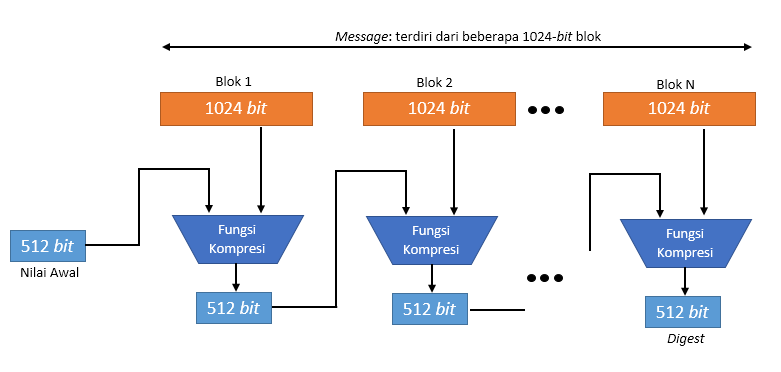
\includegraphics[scale=0.7]{Gambar/digest_creation}
	\caption{Proses Keseluruhan dari SHA-512}\label{fig:digestcreate}
\end{figure}

\section{Otentikasi}

Otentikasi adalah proses untuk menentukan keaslian identitas dari sebuah entitas saat akan mengakses sumber daya sebuah sistem. Berdasarkan entitas yang diotentikasi \cite{forouzan2007cryptography}, otentikasi dibagi menjadi 2 jenis, yaitu:

\begin{enumerate}
	\item Otentikasi pesan \\
	Otentikasi pesan adalah proses otentikasi untuk memastikan bahwa pesan berasal dari sumber data yang bisa dipercaya. Otentikasi pesan juga memastikan bahwa pesan tidak diubah saat pengiriman pesan sedang berlangsung. Beberapa teknik otentikasi pesan adalah \textit{Modification Detection Code} dan \textit{Message Authentication Code}.
	\item Otentikasi entitas \\
	Otentikasi entitas adalah proses otentikasi untuk memastikan kebenaran identitas seseorang. Entitas yang diotentikasi bisa berupa orang atau pengguna (\textit{user}). Beberapa teknik otentikasi entitas adalah \textit{password}, \textit{zero-knowledge}, \textit{challenge-response}, dan biometrik.
\end{enumerate}

Sementara itu, berdasarkan bentuknya\cite{forouzan2007cryptography}, otentikasi dibagi menjadi 3 jenis, yaitu:
\begin{enumerate}
	\item Sesuatu yang diketahui (\textit{something known}) \\
	Sesuatu yang diketahui oleh pengirim pesan dan kebenarannya bisa dipastikan oleh penerima pesan. Contohnya antara lain adalah \textit{password}, nomor PIN, \textit{passphrase}, dan sebagainya.
	\item Sesuatu yang dimiliki (\textit{something possessed}) \\
	Sesuatu yang dimiliki adalah sesuatu yang menunjukkan identitas dari pengirim pesan. Contohnya adalah paspor, KTP, kartu kredit, SIM, dan sebagainya.
	\item Sesuatu yang melekat (\textit{something inherent}) \\
	Sesuatu yang melekat adalah sesuatu yang menempel atau sebagai bagian dari pengirim pesan. Contohnya adalah sidik jari, suara, pola retina, dan sebagainya.
\end{enumerate}

\subsection{\textit{Password}}

\textit{Password} adalah sekumpulan huruf, angka, dan simbol yang sifatnya rahasia. \textit{Password} merupakan salah satu teknik dari otentikasi entitas. \textit{Password} digunakan saat seseorang hendak mengakses sumber daya sebuah sistem, seperti \textit{email}, akun media sosial, dan sebagainya. \textit{Password} ini sifatnya rahasia dan tidak boleh diketahui oleh pihak yang tidak berhak.

Berdasarkan cara penggunaannya\cite{forouzan2007cryptography}, password dibagi menjadi 2 jenis, yaitu:
\begin{enumerate}
	\item \textit{One-Time Password} \\
	\textit{One-Time Password} adalah \textit{password} yang digunakan hanya satu kali untuk setiap akses kepada sistem. Jadi, setiap kali pengguna mengakses sistem dalam sesi waktu yang berbeda, \textit{password} yang digunakan pun akan berbeda-beda. Beberapa contoh dari \textit{One-Time Password} adalah \textit{List of Passwords, Sequentially Updated Password,} dan \textit{Lamport One-Time Password}.
	\item \textit{Password} Tetap \\
	\textit{Password} tetap adalah \textit{password} yang digunakan berulang-ulang setiap kali pengguna akan mengakses sistem. \textit{Password} yang digunakan untuk mengakses sistem selalu sama. Berikut adalah beberapa skema dari \textit{password} tetap.
\end{enumerate}

\subsubsection{Skema 1}

Dalam skema ini, sistem menyimpan setiap \textit{password} pada sebuah tabel basis data. \textit{Password} yang disimpan di tabel basis data berupa \textit{plaintext}, artinya bisa dibaca dan dimengerti. Masing-masing dari \textit{password} memiliki \textit{username} yang disimpan juga di tabel basis data. Saat pengguna akan mengakses sistem, pengguna akan memasukan \textit{username} dan \textit{password}.

Kemudian, saat pengguna sudah memasukan \textit{username} dan \textit{password}, sistem akan mencari informasi dari pengguna di tabel basis data lewat \textit{username}. Karena setiap \textit{username} memiliki \textit{password}, sistem akan menyesuaikan \textit{username} dan \textit{password} di tabel basis data dengan \textit{username} dan \textit{password} yang dimasukan oleh pengguna saat hendak mengakses sistem. Jika \textit{username} dan \textit{password} yang dimasukan pengguna sesuai dengan \textit{username} dan \textit{password} di tabel basis data maka hak akses sistem akan diberikan. Gambar \ref{fig:password1} menunjukkan proses yang dijelaskan.

% diagram
\begin{figure}[H]
	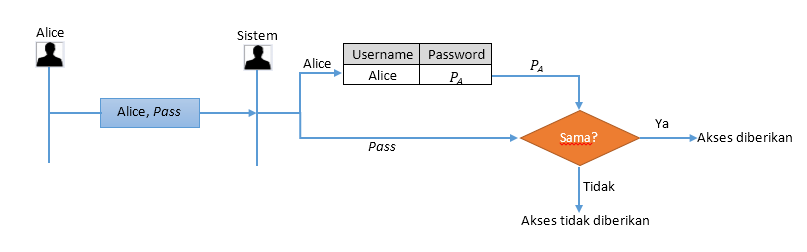
\includegraphics[scale=0.7]{Gambar/password_1}
	\centering
	\caption{\textit{Username} dan \textit{Password}}\label{fig:password1}
\end{figure}

Kelebihan dari skema ini adalah skema ini mudah untuk diimplementasikan dan tidak membutuhkan proses yang rumit. Sementara itu, kekurangan dari skema ini adalah \textit{password} yang disimpan di tabel basis data bisa dibaca dan dimengerti karena disimpan dalam bentuk \textit{plaintext}. Akibatnya, jika ada pihak yang tidak memiliki hak akses berhasil memperoleh \textit{password} yang disimpan di tabel basis data, maka \textit{password} sudah tidak rahasia lagi.

\subsubsection{Skema 2}

Dalam skema ini, sistem tetap menyimpan \textit{username} dan \textit{password} dalam tabel basis data. \textit{Password} yang disimpan tidak dalam bentuk \textit{plaintext}nya, tetapi disimpan dalam bentuk \textit{digest}nya. Saat pengguna hendak mengakses sistem, pengguna tetap memasukan \textit{username} dan \textit{password} dalam bentuk \textit{plaintext}.

Kemudian, saat pengguna sudah memasukan \textit{username} dan \textit{password}, sistem akan terlebih dahulu menghitung \textit{digest} dari \textit{password} yang dimasukan menggunakan fungsi \textit{hash}. Setelah itu, \textit{username} dan \textit{digest} akan disesuaikan dengan \textit{username} dan \textit{digest} yang disimpan dalam tabel basis data. Jika sesuai, maka pengguna akan diberikan hak akses ke sistem. Gambar \ref{fig:password2} menunjukkan proses yang sudah dijelaskan.

% diagram
\begin{figure}[H]
	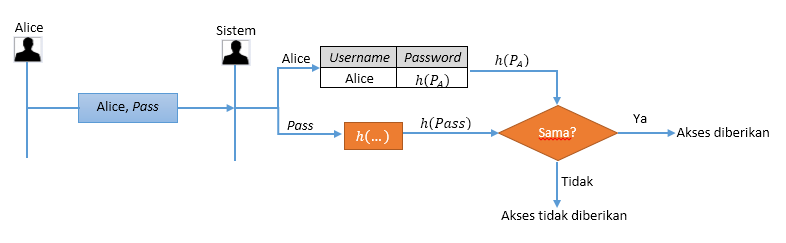
\includegraphics[scale=0.7]{Gambar/password_2}
	\centering
	\caption{\textit{Password hashing}}\label{fig:password2}
\end{figure}

Kelebihan dari skema ini adalah walaupun \textit{password} yang disimpan dalam tabel basis data diketahui oleh pihak yang tidak berhak, \textit{password} tidak akan bisa dimengerti karena disimpan dalam bentuk \textit{digest}nya. Sementara itu, \textit{digest} tidak bisa dikembalikan ke dalam bentuk \textit{plaintext} untuk mendapatkan \textit{password} karena fungsi \textit{hash} adalah fungsi satu arah seperti yang sudah dibahas dalam \ref{sec:fungsihash}. Sementara itu, kekurangan dari skema ini adalah \textit{digest} yang disimpan masih rentan terhadap \textit{dictionary attack}. Penjelasan tentang \textit{dictionary attack} akan dijelaskan pada skema selanjutnya.

\subsubsection{Skema 3}

Dalam skema 3, sistem tetap menyimpan \textit{username}. Password juga disimpan dalam bentuk \textit{digest}nya. Dalam skema ini, sebelum \textit{digest password} dibuat, \textit{password} akan dikonkatenasi dengan \textit{salt}. \textit{Salt} adalah sebuah \textit{string} acak yang bisa berisi angka, huruf, atau simbol.

Penggunaan \textit{salt} disini bertujuan untuk mengurangi tingkat keberhasilan \textit{dictionary attack}. \textit{Dictionary attack} adalah serangan dengan mencoba semua kemungkinan \textit{string} masukan untuk fungsi \textit{hash} sampai menghasilkan \textit{digest} yang sesuai. Dengan adanya penambahan \textit{salt}, maka akan mengurangi kemungkinan keberhasilan dari \textit{dictionary attack} karena banyak kemungkinan dari \textit{string} masukan akan bertambah sehingga semakin sulit untuk mendapatkan \textit{digest} yang sesuai.

Karena \textit{salt} dibutuhkan untuk mengurangi tingkat keberhasilan \textit{dictionary attack}, nilai \textit{salt} akan disimpan juga dalam tabel basis data. Kemudian, saat pengguna sudah memasukan \textit{username} dan \textit{password}, sistem akan menerima \textit{password} yang dimasukan. Selanjutnya, \textit{password} dikonkatenasi dengan \textit{salt} yang disimpan lalu sistem akan menghitung \textit{digest} dari hasil konkatenasi \textit{password} dengan \textit{salt}. Setelah itu, sistem akan membandingkan dengan \textit{digest} yang disimpan dalam tabel basis data. Jika sesuai, pengguna akan diberikan hak akses ke sistem. Gambar \ref{fig:password3} menunjukkan proses yang dijelaskan.

% diagram
\begin{figure}[H]
	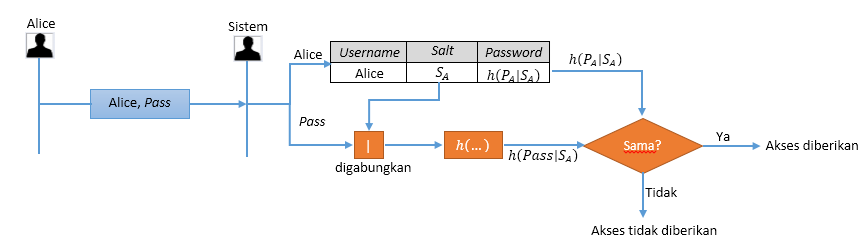
\includegraphics[scale=0.7]{Gambar/password_3}
	\centering
	\caption{\textit{Password salting}}\label{fig:password3}
\end{figure}

Kelebihan dari skema ini adalah \textit{password} tidak akan bisa diketahui dengan mudah lewat \textit{dictionary attack}. Banyak kemungkinan digest yang semakin bertambah menyebabkan serangan dengan \textit{dictionary attack} semakin sulit. Sementara itu, kekurangan dari skema ini adalah rumit karena membutuhkan banyak proses hanya untuk memberikan akses.

\section{Eliminasi Gauss-Jordan}\label{sec:eliminasigaussjordan}

Eliminasi Gauss-Jordan adalah suatu metode untuk menyelesaikan sistem persamaan linear dengan mereduksi matriks menjadi eselon baris tereduksi\cite{norman2012introduction}. Suatu matriks \begin{math}R\end{math} dikatakan bentuk eselon baris tereduksi jika memenuhi syarat sebagai berikut\cite{norman2012introduction}.

\begin{enumerate}
	\item Terdapat baris yang tidak seluruhnya terdiri dari angka 0 \\
	Angka bukan 0 pertama dari sebelah kiri dari baris tersebut disebut 1 utama.
	\item Baris yang seluruhnya terdiri dari angka 0 harus menjadi baris paling bawah.
	\item Pada kolom 1 utama, seluruh angka di bawah 1 utama harus 0.
\end{enumerate}

Sebagai contoh, matriks-matriks eselon baris tereduksi ditunjukkan oleh Matriks \ref{eq:gaussmatriks1}.

\begin{center}
	\setlength\arraycolsep{10pt}
	\begin{gather}
		\begin{bmatrix}
				1 	& 12 	& 5 	& 4 		\\[1em]
				0 	& 2 	& 4 	& 8 		\\[1em]
				0 	& 0 	& 9 	& 3
		\end{bmatrix},
		\begin{bmatrix}
				1 & 0 	\\[1em]
				0 & 1
		\end{bmatrix},
		\begin{bmatrix}
				1 	& 0 	& 2 	& 5 		\\[1em]
				0 	& 5 	& 4 	& 8 		\\[1em]
				0 	& 0 	& 4 	& 10		\\[1em]
				0 	& 0 	& 0 	& 0
		\end{bmatrix} \label{eq:gaussmatriks1}
	\end{gather}
\end{center}

Proses eliminasi Gauss-Jordan dibagi menjadi 2 proses, yaitu proses mereduksi matriks menjadi bentuk eselon baris dan proses substitusi balik ke sistem persamaan linear untuk memperoleh solusi sistem persamaan linear. Dimisalkan sistem persamaan linear yang akan dicari solusinya ditunjukkan oleh persamaan \ref{eq:gaussmatriks0}. Berikut akan dijelaskan proses mereduksi matriks menjadi bentuk eselon baris.

\begin{gather}
	x + y + z = 10 \nonumber \\
	x + 2y + 4z = 21 \label{eq:gaussmatriks0} \\
	x + 3y + 9z = 38 \nonumber
\end{gather}

\subsection{Proses Reduksi Matriks}

Proses mereduksi matriks menjadi eselon baris dilakukan dengan cara operasi baris. Operasi baris adalah suatu metode untuk mereduksi matriks menjadi eselon baris dengan cara sebagai berikut.

\begin{enumerate}
	\item Mengalikan baris dengan konstanta selain 0.
	\item Menukar 2 baris.
	\item Mengurangi sebuah baris dengan baris lainnya.
\end{enumerate}

Langkah paling awal adalah mengubah persamaan \ref{eq:gaussmatriks0} menjadi matriks. Konstanta dari variabel ke-$i$ dari persamaan ke-$j$ akan menjadi elemen matriks kolom ke-$i$ dan baris ke-$j$. Sebagai contoh, variabel ke-1 dan persamaan ke-1 dari persamaan \ref{eq:gaussmatriks0} adalah $x$ dengan konstanta 1, maka elemen matriks kolom ke-1 baris ke-1 adalah 1. Contoh lainnya, variabel ke-2 dan persamaan ke-3 persamaan \ref{eq:gaussmatriks0} adalah $3y$ dengan konstanta 3, maka elemen matriks kolom ke-2 baris ke-3 adalah 3. Hasil pengubahan persamaan \ref{eq:gaussmatriks0} menjadi matriks ditunjukkan oleh Matriks \ref{eq:gaussmatriks2}.

\begin{center}
	\setlength\arraycolsep{10pt}
	\begin{equation}
		\begin{bmatrix}
				1 	& 1 	& 1 	& 10 		\\[1em]
				1 	& 2 	& 4 	& 21 		\\[1em]
				1 	& 3 	& 9 	& 38
		\end{bmatrix} \label{eq:gaussmatriks2}
	\end{equation}
\end{center}

Operasi baris pertama adalah mengurangi baris ke-3 dan baris ke-2 dengan baris ke-1. Maka, hasil pengurangan baris ditunjukkan oleh Matriks \ref{eq:gaussmatriks3}.

\begin{center}
	\setlength\arraycolsep{10pt}
	\begin{equation}
		\begin{bmatrix}
				1 			& 1 		& 1 		& 10 				\\[1em]
				1 - 1 	& 2 - 1	& 4 - 1	& 21 - 10		\\[1em]
				1 - 1		& 3 - 1	& 9 - 1	& 38 - 10
		\end{bmatrix} \Rightarrow
		\begin{bmatrix}
				1 	& 1 	& 1 	& 10 		\\[1em]
				0 	& 1 	& 3 	& 11 		\\[1em]
				0 	& 2 	& 8 	& 28
		\end{bmatrix} \label{eq:gaussmatriks3}
	\end{equation}
\end{center}

Kemudian, operasi baris kedua adalah mengurangi baris ke-3 dengan baris ke-2 yang dikali dengan konstanta 2. Hasil operasi baris kedua ditunjukkan oleh Matriks \ref{eq:gaussmatriks4}.

\begin{center}
	\setlength\arraycolsep{10pt}
	\begin{equation}
		\begin{bmatrix}
				1 	& 1 							& 1 							& 10 		\\[1em]
				0 	& 1 							& 3 							& 11 		\\[1em]
				0 	& 2 - (1\cdot2) 	& 8 - (3\cdot2) 	& 28 - (11\cdot2)
		\end{bmatrix} \Rightarrow
		\begin{bmatrix}
				1 	& 1 	& 1 	& 10 		\\[1em]
				0 	& 1 	& 3 	& 11 		\\[1em]
				0 	& 0 	& 2 	& 6
		\end{bmatrix} \label{eq:gaussmatriks4}
	\end{equation}
\end{center}

Setelah operasi baris kedua, maka diperoleh Matriks \ref{eq:gaussmatriks5} yang merupakan matriks dengan bentuk eselon baris tereduksi.

\begin{center}
	\setlength\arraycolsep{10pt}
	\begin{equation}
		\begin{bmatrix}
				1 	& 1 	& 1 	& 10 		\\[1em]
				0 	& 1 	& 3 	& 11 		\\[1em]
				0 	& 0 	& 2 	& 6
		\end{bmatrix} \label{eq:gaussmatriks5}
	\end{equation}
\end{center}

\subsection{Proses Substitusi Balik}

Setelah mengubah matriks menjadi bentuk eselon baris tereduksi, proses substitusi balik adalah proses untuk mencari nilai koefesien dari masing-masing variabel untuk memperoleh solusi dari persamaan linear \ref{eq:gaussmatriks0}. Kolom paling kanan (kolom ke-\begin{math}n\end{math}) dari matriks menunjukkan nilai solusi dari masing-masing baris. Sementara itu, kolom ke-1 sampai kolom ke-(\begin{math}n-1\end{math}) menunjukkan koefesien dari persamaan linear.

Sebagai contoh, dari Matriks \ref{eq:gaussmatriks5} diperoleh hasilnya sebagai berikut.

\begin{gather}
	2z = 6 \nonumber \\
	z = 3 \label{eq:gaussmatriks6}
\end{gather}

Kemudian, untuk nilai \begin{math}y\end{math}.

\begin{gather}
	y + 3z = 11 \nonumber \\
	y + 3\cdot3 = 11 \nonumber \\
	y + 9 = 11 \nonumber \\
	y = 2 \label{eq:gaussmatriks7}
\end{gather}

Kemudian, untuk nilai \begin{math}x\end{math}.

\begin{gather}
	x + y + z = 10 \nonumber \\
	x + 2 + 3 = 10 \nonumber \\
	x + 5 = 10 \nonumber \\
	x = 5 \label{eq:gaussmatriks8}
\end{gather}

Jadi, solusi dari persamaan \ref{eq:gaussmatriks0} yang diselesaikan dengan eliminasi Gauss-Jordan adalah \begin{math}x=5, y=2,\end{math} dan \begin{math}z=3\end{math}.

\section{\textit{Secret Sharing} Shamir}\label{sec:secretsharingshamir}

Pada bagian ini akan dijelaskan mengenai sejarah singkat yang mengawali munculnya secret sharing Shamir dan pembahasan mengenai secret sharing Shamir.

\subsection{Sejarah Singkat}

\textit{Secret sharing} adalah metode untuk membagi informasi (rahasia) menjadi beberapa bagian. Bagian-bagian tersebut disebut \textit{share} dan setiap bagian dibagikan kepada beberapa partisipan. Untuk mendapatkan kembali informasi, maka dibutuhkan setiap \textit{share}.

Permasalahan muncul jika share dan partisipan bertambah banyak. Proses untuk mendapatkan kembali rahasia akan menjadi sulit karena setiap share harus ada. Karena permasalahan ini, pada tahun 1979 Adi Shamir memublikasikan pengembangan dari metode \textit{secret sharing} dalam esai yg berjudul '\textit{How to Share a Secret}'\cite{shamir1979share}. Metode yang dikembangkan Adi Shamir dinamakan \textit{secret sharing} Shamir.

\subsection{Pembahasan \textit{Secret Sharing} Shamir}

Untuk mengatasi permasalahan yang sudah dibahas, Shamir mengubah cara untuk mendapatkan kembali informasi. Misalkan, informasi dilambangkan dengan data \textit{D}. Dalam metode \textit{secret sharing} Shamir data \textit{D} yang dibagi menjadi \begin{math}n\end{math} \textit{share} hanya memerlukan minimal \begin{math}k\end{math} \textit{share} untuk memperoleh kembali \begin{math}D\end{math}. Skema yang dikembangkan Shamir ini dinamakan skema \textit{threshold}(\textit{k},\textit{n}),

\subsubsection{Skema \textit{Threshold}(\textit{k},\textit{n})}

Skema \textit{threshold}(\textit{k},\textit{n}) adalah skema \textit{secret sharing} dimana hanya minimal \textit{k} \textit{share} dari \textit{n} \textit{share} dibutuhkan untuk mengembalikan data \textit{D}. Skema ini memiliki ketentuan sebagai berikut\cite{shamir1979share}.

\begin{itemize}
	\item Jika \textit{share} yang dimiliki sebanyak \textit{k} \textit{share} atau lebih, \textit{D} bisa dibentuk kembali.
	\item Jika \textit{share} yang ada hanya sebanyak \textit{k-1} atau kurang maka \textit{D} tidak bisa dibentuk kembali.
\end{itemize}

Ada 2 proses dalam skema \textit{threshold}(\textit{k},\textit{n}), yaitu proses pembangunan \textit{share} dari rahasia dan proses rekonstruksi rahasia dari \textit{share} yang dimiliki. Dimisalkan rahasia adalah \begin{math}D\end{math}. Proses pertama adalah proses pembangunan \textit{share} dari \begin{math}D\end{math}. Berikut akan dijelaskan proses pembangunan \textit{share}.

\subsubsection{Proses Pembangunan \textit{Share}}

Langkah pertama adalah memilih nilai \begin{math}k\end{math}. Kemudian, setelah memilih nilai \begin{math}k\end{math} langkah selanjutnya adalah membentuk \begin{math}k-1\end{math} derajat fungsi \begin{math}f(x)\end{math}. Persamaan \ref{eq:secretsharing1} menunjukkan fungsi \begin{math}f(x)\end{math} yang dibentuk.

\begin{equation}
	f(x) = a_0 + a_1x + a_2x^2 + ... + a_{k-1}x^{k-1} \label{eq:secretsharing1}
\end{equation}

\begin{flushleft}
	dimana \begin{math}a_0 = D\end{math}.
\end{flushleft}

Setelah membentuk fungsi \begin{math}f(x)\end{math}, langkah selanjutnya adalah memilih banyak share, yaitu nilai \begin{math}n\end{math}. Setelah memilih \begin{math}n\end{math}, \begin{math}x=1\end{math} sampai \begin{math}x=n\end{math} akan dipetakan dengan fungsi \begin{math}f(x)\end{math} untuk memperoleh \begin{math}D_i\end{math}. Persamaan \ref{eq:secretsharing2} menunjukkan hasil pemetaan dengan fungsi \begin{math}f(x)\end{math}.

\begin{equation}
	D_1 = f(1), D_2 = f(2), ..., D_i = f(i), ..., D_n = f(n) \label{eq:secretsharing2}
\end{equation}

Nilai \begin{math}D_1\end{math} sampai \begin{math}D_n\end{math} adalah \textit{share} dari data \begin{math}D\end{math}.

\subsubsection{Proses Rekonstruksi Rahasia}

Pada bagian ini akan dijelaskan proses rekonstruksi \begin{math}D\end{math} dari \begin{math}D_1, D_2, ..., D_n\end{math} yang sudah dibangun dalam Proses Pembangunan \textit{Share}. Langkah pertama adalah membentuk membentuk \begin{math}k-1\end{math} derajat fungsi \begin{math}f(x)\end{math} dari \begin{math}k\end{math} yang sudah dipilih dalam Proses Pembangunan \textit{Share}. Persamaan \ref{eq:secretsharing3} menunjukkan fungsi \begin{math}f(x)\end{math} yang dibentuk.

\begin{equation}
	f(x) = a_0 + a_1x + a_2x^2 + ... + a_{k-1}x^{k-1} \label{eq:secretsharing3}
\end{equation}

Setelah itu, langkah selanjutnya adalah membentuk \begin{math}k\end{math} fungsi \begin{math}f(x)\end{math} dengan memetakan \begin{math}k\end{math} \textit{share} yang dimiliki dengan fungsi \begin{math}f(x)\end{math}. Hasil pemetaan dengan fungsi \begin{math}f(x)\end{math} ini adalah \textit{share} yang sudah dibangun pada Proses Pembangunan \textit{Share}. Persamaan \ref{eq:secretsharing4} menunjukkan hasil pemetaan masing-masing fungsi \begin{math}f(x)\end{math}.

\begin{gather}
	f(1) = a_0 + a_1\cdot 1 + a_2\cdot 1^2 + ... + a_{k-1}\cdot 1^{k-1} = D_1 \nonumber \\
	f(2) = a_0 + a_1\cdot 2 + a_2\cdot 2^2 + ... + a_{k-1}\cdot 2^{k-1} = D_2 \nonumber \\
	\vdots \nonumber \\
	f(k) = a_0 + a_1\cdot k + a_2\cdot k^2 + ... + a_{k-1}\cdot k^{k-1} = D_k \label{eq:secretsharing4}
\end{gather}

Dari hasil pemetaan yang ditunjukkan persamaan \ref{eq:secretsharing4}, langkah selanjutnya adalah membentuk persamaan linear. persamaan \ref{eq:secretsharing5} menunjukkan persamaan linear yang dibentuk.

\begin{gather}
	a_0 + a_1\cdot 1 + a_2\cdot 1^2 + ... + a_{k-1}\cdot 1^{k-1} = D_1 \qquad...\text{\textcircled{1}} \nonumber \\
	a_0 + a_1\cdot 2 + a_2\cdot 2^2 + ... + a_{k-1}\cdot 2^{k-1} = D_2 \qquad...\text{\textcircled{2}} \nonumber \\
	\vdots \nonumber \\
	a_0 + a_1\cdot k + a_2\cdot k^2 + ... + a_{k-1}\cdot k^{k-1} = D_k \qquad...\text{\textcircled{k}} \label{eq:secretsharing5}
\end{gather}

Setelah membentuk persamaan linear, langkah selanjutnya adalah menyelesaikan persamaan linear tersebut dengan metode Eliminasi Gauss-Jordan yang sudah dijelaskan pada Subbab \ref{sec:eliminasigaussjordan}. Tujuannya adalah untuk memperoleh nilai \begin{math}a_1, a_2, ..., a_{k-1}\end{math}. Dengan menggunakan Proses Substitusi Balik dalam metode Eliminasi Gauss-Jordan, dapat diperoleh nilai \begin{math}a_0\end{math} yang adalah data \begin{math}D\end{math}.

\section{Probabilitas}
Probabilitas atau peluang merupakan salah cara dalam ilmu matematika untuk mengukur tingkat kepercayaan akan suatu kejadian. Teori probabilitas sangat luas penggunaannya, baik dalam kehidupan sehari-hari maupun dalam percobaan-percobaan ilmiah. Teori probabilitas ini seringkali digunakan oleh para pengambil keputusan untuk memprediksi suatu kejadian sehingga nantinya bisa mengambil keputusan yang tepat.

Seluruh kemungkinan keluaran yang akan terjadi dalam probabilitas disebut ruang sampel sedangkan masing-masing kemungkinan yang dapat terjadi dalam ruang sampel dinamakan elemen kejadian atau anggota dari ruang sampel. Ruang sampel dilambangkan dengan huruf \begin{math}S\end{math} dan elemen kejadian dilambangkan dengan huruf \begin{math}x_i\end{math}. Dalam ruang sampel \begin{math}S\end{math} dengan \begin{math}i\end{math} elemen kejadian, ditunjukkan pada persamaan \ref{eq:probability1}.

\begin{equation}
	S = {x_1, x_2, x_3, ..., x_i}
	\label{eq:probability1}
\end{equation}

Sedangkan probabilitas kejadian \begin{math}x_i\end{math} akan terjadi dilambangkan dengan \begin{math}P(x_i)\end{math}. Maka, rumus matematikanya ditunjukkan pada persamaan \ref{eq:probability2}.

\begin{equation}
	P(x_i) = \frac{n}{N}
	\label{eq:probability2}
\end{equation}

\noindent dimana \begin{math}n\end{math} adalah banyaknya kemunculan kejadian \begin{math}x_i\end{math} dalam sebuah ruang sampel \begin{math}S\end{math} dan \begin{math}N\end{math} adalah banyaknya kejadian yang terjadi dalam ruang sampel \begin{math}S\end{math}.

\subsection{Distribusi Binom}

Setiap eksperimen atau percobaan yang dilakukan secara berkali-kali pasti memiliki dua keluaran, yaitu sukses atau gagal. Untuk setiap keluaran yang diperoleh (baik sukses maupun gagal) bisa ditetapkan sebagai sukses. Proses ini dinamakan proses Bernouli dan setiap eksperimen yang dilakukan untuk setiap proses bernouli dinamakan percobaan Bernouli. Ada beberapa syarat sebuah eksperimen bisa dinamakan percobaan Bernouli\cite{walpole1993probability}:
\begin{enumerate}
	\item Eksperimen harus diulang sebanyak \begin{math}n\end{math} kali.
	\item Hasil keluaran setiap perulangan hanya 2 kemungkinan, yaitu keluaran sukses atau keluaran gagal.
	\item Hasil keluaran setiap perulangan tidak mempengaruhi dengan perulangan yang lain.
	\item Probabilitas bahwa hasil keluarannya sukses, \begin{math}p\end{math}, harus selalu sama untuk setiap kali perulangan.
\end{enumerate}

Percobaan Bernouli digunakan untuk menghitung probabilitas \begin{math}x\end{math} buah hasil keluaran yang sukses dari \begin{math}n\end{math} percobaan. Dimisalkan bahwa probabilitas hasil keluaran setiap perulangan sukses adalah \begin{math}p\end{math}. Sebaliknya, probabilitas hasil keluaran setiap perulangan gagal adalah \begin{math}q=1-p\end{math}. Persamaan \ref{eq:binom} untuk menghitung probabilitas \begin{math}x\end{math} hasil keluaran yang sukses dari \begin{math}n\end{math} percobaan.

\begin{gather}
	P(x,n,p) = \left( {\begin{array}{c}n \\ x \end{array}} \right) p^x q^{n-x} \label{eq:binom} \\
	x = 0, 1, 2, ..., n \nonumber
\end{gather}

\begin{math}\left( {\begin{array}{c}n \\ x \end{array}} \right)\end{math} pada persamaan \ref{eq:binom} menunjukkan bahwa dari \begin{math}n\end{math} percobaan akan dipilih \begin{math}x\end{math} hasil keluaran yang sukses.

\section{Entropi}

Pada bagian ini akan dijelaskan mengenai entropi dimulai dari sejarah singkat entropi dan pembahasan mengenai entropi.

\subsection{Sejarah Singkat}

Istilah entropi muncul pertama kali dalam esai '\textit{A Mathematical Theory of Communication}' pada tahun 1948. Esai ini dibuat oleh Claude E. Shannon seorang ilmuwan asal Amerika Serikat. Dalam esainya, Shannon menulis bahwa entropi adalah konsep keacakan atau suatu ketidakpastian\cite{shannon1948mathematical}. Istilah dari entropi ini dinamakan Shannon \textit{Entropy}.

\subsection{Pembahasan}

Entropi adalah rata-rata suatu informasi yang dimiliki oleh sebuah pesan. Informasi yang dimaksud adalah kejadian yang spesifik atau sebuah elemen tertentu yang dimiliki oleh pesan. Maka dari itu, entropi bisa dijadikan alat ukur ketidakpastian yang dimiliki oleh sebuah pesan atau sumber informasi.

Nilai entropi yang tinggi menunjukkan bahwa informasi yang dimiliki sebuah pesan cukup tinggi. Nilai informasi yang cukup tinggi memiliki arti bahwa isi dari pesan bisa diprediksi. Sementara itu, jika nilai entropi yang rendah menunjukkan bahwa informasi yang dimiliki sebuah pesan cukup rendah. Nilai informasi yang cukup rendah memiliki arti bahwa isi dari pesan tidak bisa dengan mudah diprediksi.

Sebagai contoh, nilai entropi akan rendah untuk memastikan panjang umur seseorang karena tidak bisa diketahui kapan orang tersebut akan meninggal. Contoh yang lain adalah nilai entropi akan tinggi untuk kasus melemparkan koin karena hasilnya hanya ada dua kemungkinan yaitu, kepala atau buntut.

Dari penjelasan mengenai entropi yang sudah dijelaskan, dimisalkan probabilitias kemunculan informasi \begin{math}x_i\end{math} dalam sebuah pesan \begin{math}X\end{math} adalah \begin{math}p_i\end{math}. Maka, nilai entropi $x_i$ adalah \begin{math}H(x_i)\end{math} berdasarkan probabilitas kemuncul informasi $x_i$ yang dilambangkan oleh $p_i$. Persamaan \ref{eq:entropi1} menunjukkan perhitungan dari $H(x_i)$.

\begin{equation}
	H(x_i) = p_i\: log(\frac{1}{p_i})
	\label{eq:entropi1}
\end{equation}

Maka, nilai entropi pesan \begin{math}X\end{math} untuk setiap informasi \begin{math}p_1, p_2, ..., p_m\end{math} ditunjukkan oleh persamaan \ref{eq:entropi2}.

\begin{gather}
	H(X) = p_1\: log(\frac{1}{p_1}) + p_2\: log(\frac{1}{p_2}) + ... + p_m\: log(\frac{1}{p_m}) \nonumber \\
	 = \sum\limits_{i=1}^m p_i\: log(\frac{1}{p_i})
	\label{eq:entropi2}
\end{gather}}{}
\ifdefstring{\vbabc}{1}{\chapter{Analisis}
\label{chap:analisis}

Pada bab ini berisi analisis terhadap teori-teori yang telah dibahas sebelumnya. Analisis akan meliputi analisis proses, studi kasus untuk penerapan metode \textit{secret sharing} Shamir, pemilihan nilai \begin{math}n\end{math} dan \begin{math}k\end{math}, dan diagram-diagram mencakup diagram \textit{use case}, diagram aktivitas, dan rancangan diagram kelas.

\section{Analisis Proses}\label{sec:analisis}

Pada bagian ini dijelaskan mengenai perancangan perangkat lunak yang dibangun berdasarkan pada proses-proses yang sudah dipaparkan pada bagian sebelumnya. Pada bagian sebelumnya sudah dibahas mengenai proses penyimpanan \textit{password} dan proses rekonstruksi \textit{password}. Pada bagian ini dibahas setiap tahapan dari proses-proses tersebut dan setiap tahapan digambarkan dalam bentuk alur proses (\textit{flowchart}) sebelum dilakukan proses pembuatan diagram-diagram untuk membangun perangkat lunak.

\subsection{Proses Penyimpanan \textit{Password}}

Pada bagian ini dijelaskan tahapan dari proses penyimpanan \textit{password}. Flowchart dari proses penyimpanan password ditunjukkan pada Gambar \ref{fig:create_share}.

%diagram
\begin{figure}[H]
	\centerline{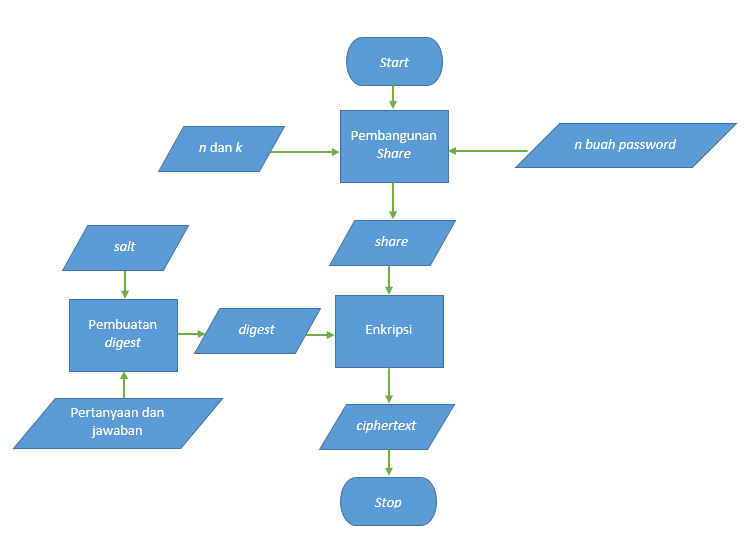
\includegraphics[scale=0.7]{Gambar/flowchart_share}}
	\caption{Proses Penyimpanan \textit{Password}}\label{fig:create_share}
\end{figure}

Tahapan-tahapan pada proses yang ditunjukkan oleh Gambar \ref{fig:create_share} adalah tahapan-tahapan untuk menyimpan \textit{password}. Dalam penelitian ini, tahapan pembangunan \textit{share} menggunakan metode \textit{secret sharing} Shamir. Berikut penjelasan masing-masing tahapan:

\begin{itemize}
	\item Tahap Pembangunan \textit{Share} \\
	Pada tahap ini, dibutuhkan data-data masukan seperti $n$, $k$, dan $n$ \textit{password}. \textit{Password} diperoleh dari masukan pengguna. $n$ diperoleh dari banyak \textit{password} yang dimasukan pengguna. $k$ ditentukan dengan cara yang sudah dijelaskan pada Subbab \ref{subsec:pilihnk}.
	\item Tahap Pembuatan Digest \\
	Pada tahap ini, dibutuhkan data-data masukan juga seperti pertanyaan keamanan, jawaban dari pertanyaan keamanan, dan \textit{salt}. Pertanyaan keamanan dan jawaban dari pertanyaan keamanan diperoleh dari masukan pengguna. Sementara itu, \textit{salt} dipilih secara acak. Setelah itu, pertanyaan, jawaban, dan \textit{salt} dikonkatenasi menjadi sebuah \textit{string} yang akan dibuat \textit{digest}nya. Dalam tahap ini, pembuatan \textit{digest} menggunakan algoritma \textit{SHA}-512 (Subbab \ref{sec:SHA512}).
	\item Tahap Enkripsi \\
	Pada tahap ini, \textit{share} yang dihasilkan pada tahap pembangunan \textit{share} dienkripsi dengan menggunakan \textit{Data Encryption Standard} (Subbab \ref{sec:des}). \textit{Digest} yang dihasilkan pada tahap pembuatan \textit{digest} akan digunakan sebagai kunci proses enkripsi. Kemudian, \textit{ciphertext} dari \textit{share} hasil enkripsi akan disimpan.
\end{itemize}

\subsection{Proses Rekonstruksi \textit{Password}}

Pada bagian ini dijelaskan tahapan dari proses rekonstruksi \textit{password}. Flowchart dari proses rekonstruksi password ditunjukkan pada Gambar \ref{fig:flowchart_reconstruct_secret}.

%diagram
\begin{figure}[H]
	\centerline{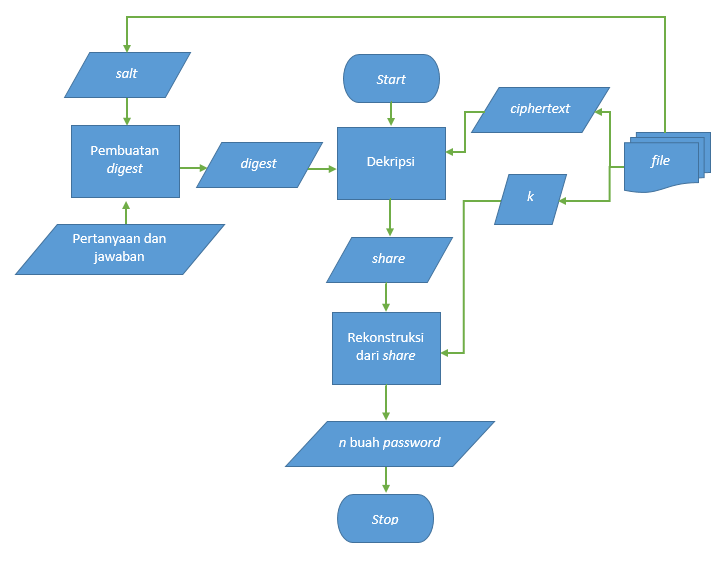
\includegraphics[scale=0.65]{Gambar/flowchart_reconstruct}}
	\caption{Proses Rekonstruksi \textit{Password}}\label{fig:flowchart_reconstruct_secret}
\end{figure}

Tahapan-tahapan pada proses yang ditunjukkan oleh Gambar \ref{fig:flowchart_reconstruct_secret} adalah tahapan-tahapan untuk merekonstruksi \textit{password}. Tujuan dari proses rekonstruksi \textit{password} adalah mengembalikan \textit{password} yang sudah disimpan. Berikut dijelaskan tahapan-tahapan dalam proses rekonstruksi \textit{password}:

\begin{itemize}
	\item Tahap Pembuatan \textit{Digest} \\
	Tahap pembuatan \textit{digest} ini sama dengan tahap pembuatan \textit{digest} dalam proses penyimpanan \textit{password}. Perbedaannya adalah pertanyaan keamanan dan nilai \textit{salt} diperoleh dari berkas teks yang disimpan. Sementara itu, jawaban dari pertanyaan keamanan tetap diperoleh dari masukan pengguna.
	\item Tahap Dekripsi \\
	Pada tahap ini, \textit{ciphertext} yang sudah disimpan akan didekripsi. Namun, sebelum proses dekripsi dilakukan, dibutuhkan beberapa data masukan \textit{digest} yang diperoleh dari tahap pembuatan \textit{digest}. Data masukan \textit{digest} digunakan sebagai kunci dalam proses dekripsi. Proses dekripsi pada tahap ini menggunakan \textit{Data Encryption Standard} (Subbab \ref{sec:des}).
	\item Tahap Rekonstruksi \textit{Share} \\
	Pada tahap ini, \textit{share} yang dihasilkan dari tahap dekripsi akan direkonstruksi untuk memperoleh \textit{password}. Tidak ada masukan pengguna dalam tahap ini. Metode rekonstruksi \textit{password} yang digunakan pada tahap ini adalah \textit{secret sharing} Shamir.
\end{itemize}

\section{Studi Kasus}

Pada bagian ini akan dibahas studi kasus tentang bagaimana penerapan metode \textit{secret sharing} Shamir untuk banyak \textit{password}. Studi kasus meliputi pengenalan kasus, proses penyimpanan \textit{password}, dan proses rekonstruksi \textit{password}.

\subsection{Pengenalan Kasus}\label{subsec:pengenalankasus}

Langkah awal yang dibutuhkan untuk mengembalikan banyak \textit{password} dengan metode \textit{secret sharing} Shamir, diperlukan beberapa tahap proses. Proses pertama adalah proses penyimpanan \textit{password}. Kemudian, proses selanjutnya adalah proses untuk mengembalikan banyak \textit{password}. Proses pertama membutuhkan beberapa \textit{password}. Untuk \begin{math}n\end{math} buah \textit{password}, maka akan dibuat \begin{math}n\end{math} buah pertanyaan keamanan. Sementara itu, untuk proses mengembalikan \textit{password} dibutuhkan pertanyaan keamanan yang sudah dibuat dalam proses sebelumnya.

Untuk kedua proses di atas, dimisalkan banyak \textit{password} yang akan disimpan sebanyak 5 buah \textit{password}. Setiap \textit{password} akan diberi label \begin{math}p_1\end{math}, \begin{math}p_2\end{math}, sampai \begin{math}p_5\end{math}. Persamaan \ref{eq:passwords1} sampai \ref{eq:passwords5} menunjukkan \begin{math}p_1\end{math} sampai \begin{math}p_5\end{math}.

\begin{gather}
	p_1 = 123456 \label{eq:passwords1} \\
	p_2 = password \label{eq:passwords2} \\
	p_3 = hello123 \label{eq:passwords3} \\
	p_4 = secret \label{eq:passwords4} \\
	p_5 = foobar \label{eq:passwords5}
\end{gather}

\subsection{Proses Penyimpanan \textit{Password}}\label{subsec:simpanpassword}

Proses penyimpanan \textit{password} dibagi menjadi 2 proses, yaitu proses pembangunan \textit{share} untuk masing-masing \textit{password} dan proses enkripsi dari setiap \textit{share} yang sudah dibangun. Pada bagian ini akan dibahas kedua proses tersebut.

\subsubsection{Proses Pembangunan \textit{Share}}

Pada proses ini, akan dilakukan pembangunan \textit{share} dari masing-masing \textit{password}. Langkah-langkah untuk membangun share adalah sebagai berikut.

\begin{enumerate}
	\item Membagi setiap \textit{password} \begin{math}p_i\end{math} menjadi beberapa karakter, masing-masing karakter akan diubah menjadi nilai ASCIInya, \begin{math}c_1, c_2, ..., c_m\end{math}.
		\item Memilih nilai \begin{math}n\end{math}, yaitu banyak \textit{share} yang akan dibangun.
	\item Memilih nilai \begin{math}k\end{math}, yaitu banyak minimal pertanyaan keamanan yang harus dijawab dengan benar, dimana \begin{math}0 < k \leq n\end{math}.
	\item Memilih \begin{math}k-1\end{math} angka acak, \begin{math}d_1, d_2, ..., d_{k-1}\end{math}, untuk masing-masing karakter \begin{math}c_1, c_2, ..., c_m\end{math}.
	\item Membentuk fungsi \begin{math}f_m(x)\end{math} untuk masing-masing karakter \begin{math}c_1, c_2, ..., c_m\end{math}. 
	Komponen dari fungsi \begin{math}f_m(x)\end{math} terdiri atas \begin{math}c_m\end{math} sebagai konstanta tanpa koefesien, \begin{math}d_1, d_2, ..., d_{k-1}\end{math} sebagai konstanta dengan koefesien. Persamaan \ref{eq:fungsifx} menunjukkan persamaan dari fungsi \begin{math}f_m(x)\end{math} yang harus dibentuk.
	\begin{equation}
		f_m(x) = c_m + d_1x + d_2x^2 + d_3x^3 + ... + d_{k-1}x^{k-1}
		\label{eq:fungsifx}
	\end{equation}
	\item Menghitung masing-masing nilai \begin{math}x\end{math} dari \begin{math}x=1, x=2, ..., x=n\end{math} untuk fungsi \begin{math}f_m(x)\end{math}.
	\item Nilai \begin{math}f_m(1)\end{math} sampai \begin{math}f_m(n)\end{math} adalah nilai \textit{share} untuk password \begin{math}p_i\end{math}.
\end{enumerate}

Kembali kepada kasus pada Subbab \ref{subsec:pengenalankasus}, misalkan \textit{password} yang akan dibangun \textit{share-share}nya adalah \begin{math}p_1\end{math}. Langkah pertama adalah membagi \begin{math}p_1\end{math} menjadi beberapa karakter dan mengubah masing-masing karakter menjadi nilai ASCIInya. Persamaan \ref{eq:ubahascii1} sampai \ref{eq:ubahascii7} menunjukkan langkah pertama.

\begin{gather}
	p_1 = 123456 \label{eq:ubahascii1} \\
	c_1 = '1' = 49 \label{eq:ubahascii2} \\
	c_2 = '2' = 50 \label{eq:ubahascii3} \\
	c_3 = '3' = 51 \label{eq:ubahascii4} \\
	c_4 = '4' = 52 \label{eq:ubahascii5} \\
	c_5 = '5' = 53 \label{eq:ubahascii6} \\
	c_6 = '6' = 54 \label{eq:ubahascii7}
\end{gather}

Langkah selanjutnya adalah memilih nilai \begin{math}n\end{math}. Karena banyak \textit{password} \begin{math}p_i\end{math} adalah 5, maka banyak \textit{share} untuk masing-masing \textit{password} sebanyak 5. Maka, \begin{math}n=5\end{math}.

Setelah memilih nilai \begin{math}n\end{math}, langkah berikutnya adalah memilih nilai \begin{math}k\end{math}. Nilai \begin{math}k\end{math} ini nanti akan berhubungan dengan banyak minimal pertanyaan keamanan yang harus dijawab benar untuk mengembalikan \textit{password}. Untuk kasus ini, dipilih \begin{math}k=3\end{math}.

Langkah selanjutnya adalah memilih \begin{math}k-1\end{math} angka acak untuk masing-masing karakter \begin{math}c_1\end{math} sampai \begin{math}c_6\end{math}. Karena \begin{math}k=3\end{math}, maka dipilih 2 angka acak untuk masing-masing karakter. Berikut angka acak untuk masing-masing karakter.

\begin{itemize}[itemsep=0mm]
	\item \begin{math}c_1\end{math}: 12 dan 6.
	\item \begin{math}c_2\end{math}: 15 dan 11.
	\item \begin{math}c_3\end{math}: 22 dan 1.
	\item \begin{math}c_4\end{math}: 21 dan 3.
	\item \begin{math}c_5\end{math}: 19 dan 8.
	\item \begin{math}c_6\end{math}: 25 dan 17.
\end{itemize}

Setelah memilih angka acak untuk masing-masing karakter, langkah selanjutnya adalah membentuk fungsi \begin{math}f(x)\end{math} untuk masing-masing karakter. Maka, fungsi \begin{math}f_1(x)\end{math} sampai \begin{math}f_6(x)\end{math} yang dibentuk adalah sebagai ditunjukkan pada persamaan \ref{eq:fungsi1} sampai \ref{eq:fungsi6}.

\begin{gather}
	f_1(x) = 49 + 12x + 6x^2 \label{eq:fungsi1} \\
	f_2(x) = 50 + 15x + 11x^2 \label{eq:fungsi2} \\
	f_3(x) = 51 + 22x + x^2 \label{eq:fungsi3} \\
	f_4(x) = 52 + 21x + 3x^2 \label{eq:fungsi4} \\
	f_5(x) = 53 + 19x + 8x^2 \label{eq:fungsi5} \\
	f_6(x) = 54 + 25x + 17x^2 \label{eq:fungsi6}
\end{gather}

Langkah selanjutnya adalah menghitung nilai \begin{math}x=1, x=2, ..., x=n\end{math} untuk fungsi \begin{math}f_1(x)\end{math} sampai \begin{math}f_6(x)\end{math}. Tabel \ref{table:itungx} menunjukkan nilai \begin{math}x=1\end{math} sampai \begin{math}x=5\end{math} untuk masing-masing fungsi \begin{math}f(x)\end{math}.

\begin{table}[H]
	\begin{center}
		\caption{Nilai \textit{x} untuk masing-masing \textit{f(x)}}\label{table:itungx}
		\begin{tabular}{| >{$}l<{$} | >{$}l<{$} | >{$}l<{$} | >{$}l<{$} | >{$}l<{$} | >{$}l<{$} | >{$}l<{$} |}
				\hline
				& f_1(x) 	& f_2(x) 	& f_3(x) 	& f_4(x) 	& f_5(x) 	& f_6(x) 	\\ \hline
			1 & 67	 		& 76 			& 74			& 76			& 80			& 96			\\ \hline
			2 & 97 			& 124			& 99			& 106			& 123			& 172			\\ \hline
			3 & 139 		& 194			& 126			& 142			& 182			& 282			\\ \hline
			4 & 193 		& 286			& 155			& 184			& 257			& 426			\\ \hline
			5 & 259 		& 400			& 186			& 232			& 348			& 604			\\ \hline
		\end{tabular}
	\end{center}
\end{table}

Setiap nilai \begin{math}x\end{math} pada Tabel \ref{table:itungx} adalah nilai \textit{share-share} untuk password \begin{math}p_1\end{math}. Setiap nilai \begin{math}x\end{math} ini akan diberi label \begin{math}s_{11}\end{math} untuk \textit{share} pertama dari fungsi pertama, \begin{math}s_{21}\end{math} untuk \textit{share} kedua dari fungsi pertama, dan seterusnya sampai \begin{math}s_{56}\end{math} untuk \textit{share} kelima dari fungsi keenam. Nilai \textit{share} yang sudah diberi label ditunjukkan pada persamaan \ref{eq:nilaishare}.

\begin{equation}
	s_{11} = 67, s_{21} = 97, ..., s_{34} = 155, ..., s_{56} = 604 \label{eq:nilaishare}
\end{equation}

Sementara itu, untuk menghitung nilai share dari \textit{password} \begin{math}p_2\end{math} sampai \begin{math}p_5\end{math}, proses yang sama untuk menghitung \textit{password} \begin{math}p_1\end{math} akan dilakukan. Setelah menghitung nilai \textit{share} untuk \textit{password} \begin{math}p_1\end{math}, langkah selanjutnya adalah proses enkripsi masing-masing \textit{share} ini.

\subsubsection{Proses Enkripsi \textit{Share}}

Pada proses ini, sebelum masing-masing \textit{share} disimpan, masing-masing \textit{share} harus dienkripsi terlebih dahulu. Dalam proses ini juga, \begin{math}n\end{math} buah pertanyaan keamanan akan dibuat. Langkah-langkah proses enkripsi \textit{share} adalah sebagai berikut.

\begin{enumerate}
	\item Membuat \begin{math}n\end{math} pertanyaan keamanan, \begin{math}q_1, q_2, ..., q_n\end{math}.
	\item Menentukan jawaban dari masing-masing pertanyaan keamanan, \begin{math}a_1, a_2, ..., a_n\end{math}.
	\item Menentukan nilai \textit{salt}, \begin{math}r_s\end{math}.
	\item Menghitung \textit{digest} untuk masing-masing konkatenasi dari pertanyaan, jawaban, dan \textit{salt}. Persamaan \ref{eq:itunghash} menunjukkan proses menghitung \textit{digest}.
	\begin{equation}
		h_n = H(q_n + a_n + r_s) \label{eq:itunghash}
	\end{equation}
	\item Setiap nilai \textit{share}, \begin{math}s_{11}, s_{21}, ..., s_{56}\end{math} akan dienkripsi dengan menggunakan digest sebagai kunci. Persamaan \ref{eq:enkripsishare1} menunjukkan langkah enkripsi \textit{share}.
	\begin{equation}
		E_{h_n}(s_{nm}) = c_{nm}\label{eq:enkripsishare1}
	\end{equation}
	Pada persamaan \ref{eq:enkripsishare1}, \begin{math}m\end{math} merupakan banyak karakter dari masing-masing \textit{password} \begin{math}p_i\end{math}.
\end{enumerate}

Kembali kepada kasus pada Subbab \ref{subsec:pengenalankasus}, misalkan \textit{password} yang akan dienkripsi \textit{share-share}nya adalah \begin{math}p_1\end{math}. Langkah pertama adalah membuat \begin{math}n\end{math} pertanyaan keamanan, karena \begin{math}n=5\end{math} maka ada 5 pertanyaan keamanan. Setiap pertanyaan keamanan akan diberi label \begin{math}q_1, q_2, ..., q_5\end{math}. Untuk kasus ini, dimisalkan pertanyaan keamanan yang dibuat adalah sebagai berikut.

\begin{enumerate}[itemsep=0mm]
	\item Siapa nama anda? (\begin{math}q_1\end{math})
	\item Dimana kota tempat anda tinggal? (\begin{math}q_2\end{math})
	\item Apa jenis kelamin anda? (\begin{math}q_3\end{math})
	\item Pada bulan apa anda lahir? (\begin{math}q_4\end{math})
	\item Apa nama belakang anda? (\begin{math}q_5\end{math})
\end{enumerate}

Setelah membuat pertanyaan keamanan yang akan digunakan, langkah selanjutnya adalah menentukan jawaban dari masing-masing pertanyaan keamanan. Setiap jawaban untuk pertanyaan keamanan akan diberi label \begin{math}a_1\end{math} untuk \begin{math}q_1\end{math}, \begin{math}a_2\end{math} untuk \begin{math}q_2\end{math}, dan seterusnya sampai \begin{math}a_5\end{math} untuk \begin{math}q_5\end{math}. Jawaban dari masing-masing pertanyaan keamanan adalah sebagai berikut.

\begin{enumerate}[itemsep=0mm]
	\item Samuel (\begin{math}a_1\end{math})
	\item Bandung (\begin{math}a_2\end{math})
	\item Laki-laki (\begin{math}a_3\end{math})
	\item Juli (\begin{math}a_4\end{math})
	\item Christian (\begin{math}a_5\end{math})
\end{enumerate}

Langkah selanjutnya adalah memilih nilai \textit{salt}, \begin{math}r_s\end{math}. Untuk kasus ini, misalkan \begin{math}r_s=31\end{math}.

Setelah memilih nilai \textit{salt}, langkah selanjutnya adalah menghitung \textit{digest}. Masing-masing dari pertanyaan keamanan akan dikonkatenasi dengan jawabannya dan \begin{math}r_s\end{math}. Contoh hasil penghitungan \textit{digest}, \begin{math}h_n\end{math}, untuk setiap pertanyaan ditunjukkan pada persamaan \ref{eq:itungdigest1} sampai \ref{eq:itungdigest5}.

\begin{gather}
	h_1 = (q_1 + a_1 + r_s) = 7a916 \label{eq:itungdigest1} \\
	h_2 = (q_2 + a_2 + r_s) = cdc62 \label{eq:itungdigest2} \\
	h_3 = (q_3 + a_3 + r_s) = de09b \label{eq:itungdigest3} \\
	h_4 = (q_4 + a_4 + r_s) = d1320 \label{eq:itungdigest4} \\
	h_5 = (q_5 + a_5 + r_s) = b59e9 \label{eq:itungdigest5}
\end{gather}

Langkah selanjutnya adalah mengenkripsi setiap nilai \textit{share} yang sudah dibangun dengan \textit{digest} yang sudah dihitung sebagai kuncinya. Contoh hasil enkripsi setiap \textit{share} untuk \begin{math}p_1\end{math}, ditunjukkan pada Tabel \ref{table:enkripsi1}.

\begin{table}[H]
	\begin{center}
		\caption{Hasil Enkripsi setiap \textit{Share} untuk \textit{Password} Pertama}\label{table:enkripsi1}
		\begin{tabular}{| >{$}l<{$} | >{$}l<{$} | >{$}l<{$} | >{$}l<{$} | >{$}l<{$} | >{$}l<{$} | >{$}l<{$} |}
				\hline
						& c_1 		& c_2 		& c_3 		& c_4 		& c_5 		& c_6 	\\ \hline
				s_1 & aa7cm	 	& a45sf 	& 1xz5q		& x15z6		& cx96v		& 6zx51		\\ \hline
				s_2 & ff3ds 	& 5cv1s		& rf51s		& xcq89		& a9er8		& 9wrt8		\\ \hline
				s_3 & fg9e5 	& afa65		& ge65r		& we65q		& s6dv5		& xf8xj		\\ \hline
				s_4 & d3d64 	& eq89v		& 85vbn		& nm6f5		& 51gvq		& x91qw		\\ \hline
				s_5 & a54q1 	& z1x56		& as46c		& na6e5		& cz98q		& ha658		\\ \hline
		\end{tabular}
	\end{center}
\end{table}

Kolom pada Tabel \ref{table:enkripsi1} menunjukkan urutan karakter dari \textit{password}. Sementara itu, baris menunjukkan urutan \textit{share} dari masing-masing karakter. Sebagai contoh, kolom $c_1$ baris $s_1$ menunjukkan hasil enkripsi untuk \textit{share} pertama dari karakter pertama \textit{password} $p_1$.

Langkah enkripsi setiap \textit{share} ini dilakukan untuk setiap \textit{password} \begin{math}p_2\end{math} sampai \begin{math}p_5\end{math}. Kemudian setelah proses enkripsi ini, pertanyaan keamanan, jawaban, hasil enkripsi (\textit{ciphertext}), nilai \textit{salt}, dan nilai \begin{math}k\end{math} akan disimpan.

\subsection{Proses Pengembalian \textit{Password}}

Setelah \textit{password} disimpan dalam proses Penyimpanan \textit{Password} (Subbab \ref{subsec:simpanpassword}), pada bagian ini akan dijelaskan proses bagaimana \textit{password} bisa dikembalikan dengan menggunakan metode \textit{secret sharing} Shamir. Proses pengembalian \textit{password} ini dibagi menjadi 2 proses, yaitu proses dekripsi setiap \textit{share} dan proses rekonstruksi kembali \textit{password} dari \textit{share-share} yang sudah didekripsi.

\subsubsection{Proses Dekripsi \textit{Share}}

Proses dekripsi \textit{share} adalah proses mengembalikan \textit{ciphertext} dari masing-masing \textit{share} kembali kepada bentuk \textit{plaintext}nya. Langkah-langkah dari proses dekripsi \textit{share} adalah sebagai berikut.

\begin{enumerate}
	\item Menjawab \begin{math}n\end{math} pertanyaan keamanan yang sebelumnya disimpan, \begin{math}q_1, q_2, ..., q_n\end{math} untuk menghasilkan jawaban \begin{math}a'_1, a'_2, ..., a'_n\end{math}.
	\item Menghitung \textit{digest} untuk masing-masing konkatenasi dari pertanyaan yang disimpan, jawaban, dan \textit{salt} yang disimpan. Persamaan \ref{eq:itunghashbalik} menunjukkan proses menghitung \textit{digest}.
	\begin{equation}
		h'_n = H(q_n + a'_n + r_s) \label{eq:itunghashbalik}
	\end{equation}
	\item Mendekripsi \begin{math}c_{11}, c_{21}, ..., c{nm}\end{math} dengan menggunakan \begin{math}h'_1, h'_2, ..., h'_n\end{math} sebagai kunci. Persamaan \ref{eq:dekripsibalik} menunjukkan langkah yang dijelaskan.
	\begin{equation}
		D_{h'_n}(c_{nm}) = s'_{nm} \label{eq:dekripsibalik}
	\end{equation}
\end{enumerate}

Kembali kepada kasus yang dijelaskan pada Subbab \ref{subsec:pengenalankasus}, langkah pertama adalah menjawab pertanyaan keamanan yang sebelumnya disimpan. Berikut pertanyaan keamanan yang disimpan dan jawaban untuk masing-masing pertanyaan keamanan.

\begin{enumerate}[itemsep=0mm]
	\item Siapa nama anda? (\begin{math}q_1\end{math}): Samuel (\begin{math}a'_1\end{math})
	\item Dimana kota tempat anda tinggal? (\begin{math}q_2\end{math}): Bandung (\begin{math}a'_2\end{math})
	\item Apa jenis kelamin anda? (\begin{math}q_3\end{math}): Laki-laki (\begin{math}a'_3\end{math})
	\item Pada bulan apa anda lahir? (\begin{math}q_4\end{math}): Juli (\begin{math}a'_4\end{math})
	\item Apa nama belakang anda? (\begin{math}q_5\end{math}): Christian (\begin{math}a'_5\end{math})
\end{enumerate}

Kemudian, langkah selanjutnya adalah menghitung \textit{digest} masing-masing konkatenasi dari pertanyaan yang disimpan, jawaban, dan \textit{salt} yang disimpan, \begin{math}r_s=31\end{math}. Contoh hasil penghitungan \textit{digest}, \begin{math}h'_n\end{math}, untuk setiap pertanyaan ditunjukkan pada persamaan \ref{eq:itungdigestbalik1} sampai \ref{eq:itungdigestbalik5}.

\begin{gather}
	h'_1 = (q_1 + a'_1 + r_s) = 7a916 \label{eq:itungdigestbalik1} \\
	h'_2 = (q_2 + a'_2 + r_s) = cdc62 \label{eq:itungdigestbalik2} \\
	h'_3 = (q_3 + a'_3 + r_s) = de09b \label{eq:itungdigestbalik3} \\
	h'_4 = (q_4 + a'_4 + r_s) = d1320 \label{eq:itungdigestbalik4} \\
	h'_5 = (q_5 + a'_5 + r_s) = b59e9 \label{eq:itungdigestbalik5}
\end{gather}

Setelah memperoleh \textit{digest}, langkah selanjutnya adalah mendekripsi setiap \textit{share} dalam Tabel \ref{table:enkripsi1} dengan \textit{digest} \begin{math}h'1, h'2, ..., h'5\end{math} sebagai kunci. Persamaan \ref{eq:dekripsishare1} dan \ref{eq:dekripsishare2} menunjukkan langkah dari dekripsi salah satu \textit{share}.

\begin{gather}
	c_{11} = aa7cm \label{eq:dekripsishare1} \\
	D_{h_1}(c_{11}) = s_{11} = 67 \label{eq:dekripsishare2}
\end{gather}

Kemudian, proses dekripsi diulang untuk setiap \textit{share} dari \textit{password} \begin{math}p_1\end{math}. Tabel \ref{table:tabeldekripsi1} menunjukkan hasil dari dekripsi setiap \textit{share}.

\begin{table}[H]
	\begin{center}
		\caption{Hasil Dekripsi \textit{Share}}\label{table:tabeldekripsi1}
		\begin{tabular}{| >{$}l<{$} | >{$}l<{$} | >{$}l<{$} | >{$}l<{$} | >{$}l<{$} | >{$}l<{$} | >{$}l<{$} |}
				\hline
						& c_1		 	& c_2		 	& c_3		 	& c_4		 	& c_5		 	& c_6		 	\\ \hline
				s_1 & 67	 		& 76 			& 74			& 76			& 80			& 96			\\ \hline
				s_2 & 97 			& 124			& 99			& 106			& 123			& 172			\\ \hline
				s_3 & 139 		& 194			& 126			& 142			& 182			& 282			\\ \hline
				s_4 & 193 		& 286			& 155			& 184			& 257			& 426			\\ \hline
				s_5 & 259 		& 400			& 186			& 232			& 348			& 604			\\ \hline
		\end{tabular}
	\end{center}
\end{table}

Kolom pada Tabel \ref{table:tabeldekripsi1} menunjukkan urutan karakter dari \textit{password} \begin{math}p_1\end{math}, sedangkan baris pada Tabel \ref{table:tabeldekripsi1} menunjukkan urutan \textit{share} untuk masing-masing karakter. Sebagai contoh, baris \begin{math}s_1\end{math} kolom $c_1$ menunjukkan \textit{share} pertama untuk karakter pertama dari \textit{password} \begin{math}p_1\end{math} dan seterusnya sampai baris \begin{math}s_5\end{math} kolom $c_6$ menunjukkan \textit{share} kelima untuk karakter keenam \textit{password} \begin{math}p_1\end{math}.

\subsubsection{Proses Rekonstruksi \textit{Password}}

Setelah memperoleh hasil dekripsi \textit{share} untuk masing-masing karakter dari masing-masing \textit{password} \begin{math}p_1\end{math} sampai \begin{math}p_5\end{math}, proses selanjutnya adalah proses rekonstruksi masing-masing \textit{password}. Dalam kasus ini, \textit{password} yang akan direkonstruksi adalah \begin{math}p_1\end{math}. Berikut langkah-langkah dari rekonstruksi \begin{math}p_i\end{math}.

\begin{enumerate}
	\item Membentuk fungsi dasar \begin{math}f(x)\end{math} untuk masing-masing karakter dari \textit{password} \begin{math}p_i\end{math} berdasarkan nilai \begin{math}k\end{math} yang disimpan. Nilai \begin{math}k\end{math} mempengaruhi derajat dari fungsi \begin{math}f(x)\end{math} yang akan dibentuk. Persamaan \ref{eq:fungsifxbalik} menunjukkan fungsi \begin{math}f(x)\end{math} yang akan dibentuk.
	\begin{equation}
		f(x) = a_0 + a_1x + a_2x^2 + ... + a_{k-1}x^{k-1} \label{eq:fungsifxbalik}
	\end{equation}
	\item Setiap karakter dari \textit{password} \begin{math}p_i\end{math} diwakili oleh 1 fungsi \begin{math}f(x)\end{math}. Maka, untuk setiap karakter dibentuk fungsi \begin{math}f_m(x)\end{math} masing-masing, dimana \begin{math}m\end{math} adalah banyak karakter dari \textit{password} \begin{math}p_i\end{math}. Persamaan \ref{eq:fungsimasingmasing} menunjukkan langkah yang dijelaskan.
	\begin{equation}
		f_m(x) = a_0 + a_1x + a_2x^2 + ... + a_{k-1}x^{k-1} \label{eq:fungsimasingmasing}
	\end{equation}
	\item Menghitung nilai \textit{share} yang dimiliki untuk masing-masing fungsi \begin{math}f(x)\end{math} setiap karakter. Persamaan \ref{eq:fxkaraktershare} menunjukkan langkah yang dijelaskan.
	\begin{equation}
		f_m(n) = a_0 + a_1n + a_2n^2 + ... + a_{k-1}n^{k-1} = s_{nm} \label{eq:fxkaraktershare}
	\end{equation}
	\item Menghitung konstanta bebas dari berdasarkan fungsi \begin{math}f(x)\end{math} yang ada untuk masing-masing karakter, dari \begin{math}f_1(x), f_2(x), ..., f_m(x)\end{math}.
	\item Mengubah konstanta bebas yang diperoleh dari langkah sebelumnya menjadi karakter ASCII.
\end{enumerate}

Setelah diperoleh nilai setiap \textit{share} yang ditunjukkan pada Tabel \ref{table:tabeldekripsi1}, langkah pertama yang dilakukan untuk mengembalikan \textit{password} adalah membentuk fungsi dasar \begin{math}f(x)\end{math} untuk masing-masing karakter dari password \begin{math}p_i\end{math} berdasarkan nilai \begin{math}k\end{math} yang disimpan. Dalam kasus Subbab \ref{subsec:pengenalankasus}, \begin{math}k\end{math} yang dipilih adalah \begin{math}k=3\end{math}, maka fungsi \begin{math}f(x)\end{math} yang dibentuk memiliki derajat \begin{math}k-1\end{math}. Persamaan \ref{eq:fungsifxkarakter} menunjukkan fungsi \begin{math}f(x)\end{math} yang dibentuk.

\begin{equation}
	f(x) = c + bx + ax^2 \label{eq:fungsifxkarakter}
\end{equation}

Langkah selanjutnya adalah membentuk fungsi \begin{math}f(x)\end{math} untuk setiap karakter \textit{password} \begin{math}p_1\end{math}. Persamaan \ref{eq:fungsifxkarakter1} sampai \ref{eq:fungsifxkarakter6} menunjukkan fungsi \begin{math}f(x)\end{math} untuk setiap karakter \textit{password} \begin{math}p_1\end{math}.

\begin{align}
	f_1(x) = c + bx + ax^2 \label{eq:fungsifxkarakter1} \\
	f_2(x) = c + bx + ax^2 \label{eq:fungsifxkarakter2} \\
	f_3(x) = c + bx + ax^2 \label{eq:fungsifxkarakter3} \\
	f_4(x) = c + bx + ax^2 \label{eq:fungsifxkarakter4} \\
	f_5(x) = c + bx + ax^2 \label{eq:fungsifxkarakter5} \\
	f_6(x) = c + bx + ax^2 \label{eq:fungsifxkarakter6}
\end{align}

Setelah itu, langkah selanjutnya adalah menghitung nilai \textit{share} yang dimiliki pada fungsi \begin{math}f(x)\end{math} yang sudah dibentuk. Untuk langkah ini, akan ditunjukkan proses pengembalian salah satu karakter dari \textit{password} \begin{math}p_1\end{math}, yaitu karakter pertama.

Dimisalkan \textit{share} yang digunakan untuk rekonstruksi karakter pertama adalah \begin{math}s_{11}, s_{21}, \end{math} dan \begin{math}s_{31}\end{math}. Maka, nilai masing-masing share ini pada fungsi \begin{math}f_1(x)\end{math} ditunjukkan pada persamaan \ref{eq:karakterpertamafx1} sampai \ref{eq:karakterpertamafx3}.

\begin{align}
	f_1(1) = c + b + a = 67 \label{eq:karakterpertamafx1} \\
	f_1(2) = c + 2b + 4a = 97 \label{eq:karakterpertamafx2} \\
	f_1(3) = c + 3b + 9a = 139 \label{eq:karakterpertamafx3}
\end{align}

Langkah selanjutnya adalah menghitung konstanta bebas, yaitu dalam kasus ini konstanta bebas \begin{math}c\end{math}. Proses eliminasi Gauss-Jordan digunakan dalam menghitung konstanta bebas. Langkah pertama adalah transformasi \begin{math}f_1(x), f_2(x),\end{math} dan \begin{math}f_3(x)\end{math} menjadi matriks. Matriks \ref{eq:gauss1} menunjukkan hasil tranformasi \begin{math}f_1(x), f_2(x),\end{math} dan \begin{math}f_3(x)\end{math}.

\begin{center}
	\setlength\arraycolsep{10pt}
	\begin{equation}
		\begin{bmatrix}
				1 	& 1 	& 1 	& 67 		\\[1em]
				1 	& 2 	& 4 	& 97 		\\[1em]
				1 	& 3 	& 9 	& 139
		\end{bmatrix}
		\label{eq:gauss1}
	\end{equation}
\end{center}

Kolom paling kanan dari Matriks \ref{eq:gauss1} menunjukkan nilai \begin{math}f_1(x), f_2(x),\end{math} dan \begin{math}f_3(x)\end{math}, sedangkan kolom lainnya menunjukkan nilai koefesien dari setiap variabel dalam \begin{math}f_1(x), f_2(x),\end{math} dan \begin{math}f_3(x)\end{math}. Kemudian, setiap baris akan diberi label. Baris 1 diberi label \begin{math}L_1\end{math}, baris 2 diberi label \begin{math}L_2\end{math}, dan baris 3 diberi label \begin{math}L_3\end{math}.

Setelah transformasi matriks, langkah selanjutnya adalah operasi setiap baris untuk memperoleh matriks bentuk eselon baris tereduksi. Operasi pertama yang dilakukan ditunjukkan oleh persamaan \ref{eq:gauss2}.

\begin{gather}
	L_3 - L_1 \nonumber \\
	L_2 - L_1 \label{eq:gauss2}
\end{gather}

\begin{flushleft}
	Operasi pertama menghasilkan Matriks \ref{eq:gauss3}.
\end{flushleft}

\begin{center}
	\setlength\arraycolsep{10pt}
	\begin{equation}
		\begin{bmatrix}
				1 	& 1 	& 1 	& 67 		\\[1em]
				0 	& 1 	& 3 	& 30 		\\[1em]
				0 	& 2 	& 8 	& 72
		\end{bmatrix}
		\label{eq:gauss3}
	\end{equation}
\end{center}

Langkah selanjutnya adalah operasi baris kembali sampai memperoleh matriks bentuk eselon baris tereduksi. Operasi kedua ditunjukkan pada persamaan \ref{eq:gauss4}.

\begin{equation}
	L_3 - 2L_2 \label{eq:gauss4}
\end{equation}

\begin{flushleft}
	Operasi kedua menghasilkan Matriks \ref{eq:gauss5}.
\end{flushleft}

\begin{center}
	\setlength\arraycolsep{10pt}
	\begin{equation}
		\begin{bmatrix}
				1 	& 1 	& 1 	& 67 		\\[1em]
				0 	& 1 	& 3 	& 30 		\\[1em]
				0 	& 0 	& 2 	& 12
		\end{bmatrix}
		\label{eq:gauss5}
	\end{equation}
\end{center}

Setelah operasi kedua, diperoleh matriks segitiga atas yang ditunjukkan oleh Matriks \ref{eq:gauss5}. Langkah selanjutnya setelah memperoleh matriks bentuk eselon baris tereduksi adalah substitusi balik untuk memperoleh masing-masing nilai koefesien untuk setiap variabel \begin{math}a, b,\end{math} dan \begin{math}c\end{math}. Proses substitusi balik pertama adalah untuk memperoleh nilai \begin{math}a\end{math}. Persamaan \ref{eq:gauss6} menunjukkan proses substitusi balik pertama.

\begin{align}
	2a = 12 \nonumber \\
	a = 6 \label{eq:gauss6}
\end{align}

Proses substitusi balik kedua adalah untuk memperoleh nilai \begin{math}b\end{math}. Proses substitusi balik kedua ditunjukkan pada persamaan \ref{eq:gauss7}.

\begin{align}
	b + 3a = 30 \nonumber \\
	b + 3\cdot6 = 30 \nonumber \\
	b + 18 = 30 \nonumber \\
	b = 12 \label{eq:gauss7}
\end{align}

Proses substitusi balik ketiga adalah untuk memperoleh nilai \begin{math}c\end{math}. Proses substitusi balik ketiga ditunjukkan pada persamaan \ref{eq:gauss8}.

\begin{align}
	c + b + a = 67 \nonumber \\
	c + 12 + 6 = 67 \nonumber \\
	c + 18 = 67 \nonumber \\
	c = 49 \label{eq:gauss8}
\end{align}

Setelah proses substitusi balik ketiga diperoleh konstanta bebas \begin{math}c=49\end{math} untuk karakter pertama. Langkah selanjutnya setelah memperoleh konstanta bebas adalah mengubah konstanta bebas menjadi karakter ASCII. Karakter ASCII ke-49 adalah '1'. Maka, untuk karakter pertama dari \begin{math}p_1\end{math} adalah '1'.

Proses yang sama akan dilakukan untuk karakter kedua, ketiga, sampai karakter keenam. Setelah semua karakter diperoleh, setiap karakter akan dikonkatenasi menjadi sebuah \textit{string}. Maka, hasil akhir dari \begin{math}p_1\end{math} ditunjukkan pada persamaan \ref{eq:passwordbalik1}.

\begin{equation}
	p_1 = 123456 \label{eq:passwordbalik1}
\end{equation}

\section{Pemilihan Nilai \textit{n} dan \textit{k}}\label{subsec:pilihnk}

Pengguna dapat memilih \begin{math}n\end{math} dan \begin{math}k\end{math} sesuai dengan kebutuhan. Pemilihan \begin{math}n\end{math} dan \begin{math}k\end{math} yang baik, tidak hanya dapat membuat \textit{password} tidak akan mudah dikembalikan oleh pihak yang tidak berhak, tetapi dapat juga membuat pengguna bisa dengan mudah mengembalikan \textit{password}\cite{ellison2000protecting}. Pada bagian ini, akan dijelaskan bagaimana pemilihan \begin{math}n\end{math} dan \begin{math}k\end{math} dapat mempengaruhi kedua hal tersebut.

\subsection{Pemilihan Nilai \textit{k}}

Nilai \begin{math}k\end{math} adalah banyak minimal pertanyaan benar yang perlu dijawab agar bisa memperoleh \textit{password}. Setiap dari pertanyaan keamanan memiliki kemungkinan jawabannya masing-masing. Setiap pertanyaan keamanan ini memiliki nilai entropi \begin{math}e_i\end{math} dilihat dari kemungkinan jawaban setiap pertanyaan. Jenis pertanyaan keamanan yang dibuat akan mempengaruhi nilai entropi $e_i$.

Maka dengan bertambahnya nilai \begin{math}k\end{math} dan diasumsikan \begin{math}e_i\end{math} dari setiap pertanyaan sangat kecil, maka kemungkinan jawaban dari setiap pertanyaan akan bervariasi sehingga jawaban dari masing-masing pertanyaan keamanan tidak bisa dengan mudah ditebak atau diprediksi. Namun, nilai \begin{math}k\end{math} yang terlalu besar juga akan menyulitkan pemilik \textit{password} untuk mengembalikan \textit{password} karena semakin banyak pertanyaan yang harus dijawab dengan tepat.

\subsection{Pemilihan Nilai \textit{n}}

Nilai \begin{math}n\end{math} adalah banyak pertanyaan keamanan yang dibuat. Banyak pertanyaan yang dibuat, $n$, memiliki hubungan yang erat dengan kemampuan pengguna menjawab setiap pertanyaan dengan benar. Diasumsikan jika probabilitas sebuah pertanyaan dijawab dengan benar adalah $P_0$. Maka, probabilitas bahwa pengguna bisa menjawab benar $k$ pertanyaan dari $n$ pertanyaan\cite{ellison2000protecting}:

\begin{equation}
	P_1(k,n,P_0) = \left(\begin{array}{c}n\\k\end{array}\right) P_0^k (1-P_0)^{n-k}
	\label{eq:pilihn1}
\end{equation}

Maka, dari persamaan \ref{eq:pilihn1} untuk $n$ pertanyaan, probabilitas dari $P_i$ akan bertambah besar dengan bertambah besarnya nilai $k$. Melalui hal tersebut, dapat disimpulkan probabilitas pengguna akan berhasil mengembalikan \textit{password}\cite{ellison2000protecting}:

\begin{equation}
	P_2(k,n,P_0) = \sum\limits_{i=k}^n P_1(i,n,P_0)
	\label{eq:pilihn2}
\end{equation}

$P_2$ akan mempengaruhi pasangan $n$ dan $k$ yang harus dipilih. Jika dimisalkan $P_0 = 0.95$ dan $P_2 = 0.99998$, maka pasangan $n$ dan $k$ yang ideal dari hasil penghitungan menggunakan persamaan \ref{eq:pilihn2}\cite{ellison2000protecting}:

\begin{table}[H]
	\begin{center}
		\caption{Tabel Pasangan Nilai $n$ dan $k$}\label{table:pilihn3}
		\begin{tabular}{|| >{$}c<{$} | >{$}c<{$} || >{$}c<{$} | >{$}c<{$} || >{$}c<{$} | >{$}c<{$} ||}
				\hline
				n		& k		 		& n		 	& k				& n		& k 				\\ \hline
				5 	& 1	 			& 6 		& 1				& 7		& 1..2			\\ \hline
				8 	& 1..3 		& 9			& 1..3		& 10	& 1..4			\\ \hline
				11 	& 1..5 		& 12		& 1..6		& 13	& 1..7			\\ \hline
				14 	& 1..7 		& 15		& 1..8		& 16	& 1..9			\\ \hline
				17 	& 1..10 	& 18		& 1..11		& 19	& 1..11			\\ \hline
				20 	& 1..12 	& 21		& 1..13		& 22	& 1..14			\\ \hline
				23 	& 1..15 	& 24		& 1..16		& 25	& 1..17			\\ \hline
				26 	& 1..17 	& 27		& 1..18		& 28	& 1..19			\\ \hline
				29 	& 1..20 	& 30		& 1..21		& ...	& ...				\\ \hline
		\end{tabular}
	\end{center}
\end{table}

\section{Diagram}

Pada bagian ini dibuat diagram-diagram untuk perangkat lunak yang dibangun. Diagram-diagram ini dibuat berdasarkan analisis proses yang sudah dijelaskan pada Subbab \ref{sec:analisis}.

\subsection{Diagram \textit{Use Case}}

Perangkat lunak yang dibangun memiliki 2 fitur utama, yaitu menyimpan \textit{password} beserta pertanyaan keamanan yang sifatnya personal dan mengembalikan \textit{password}. Saat menyimpan \textit{password}, pengguna akan diminta untuk menambahkan pertanyaan keamanan yang sifatnya personal dan saat mengembalikan \textit{password}, pengguna akan diminta untuk menjawab pertanyaan keamanan yang sudah disimpan saat menyimpan \textit{password}. Gambar \ref{fig:use_case} menunjukkan diagram \textit{use case} dari perangkat lunak.

%diagram
\begin{figure}[H]
	\centerline{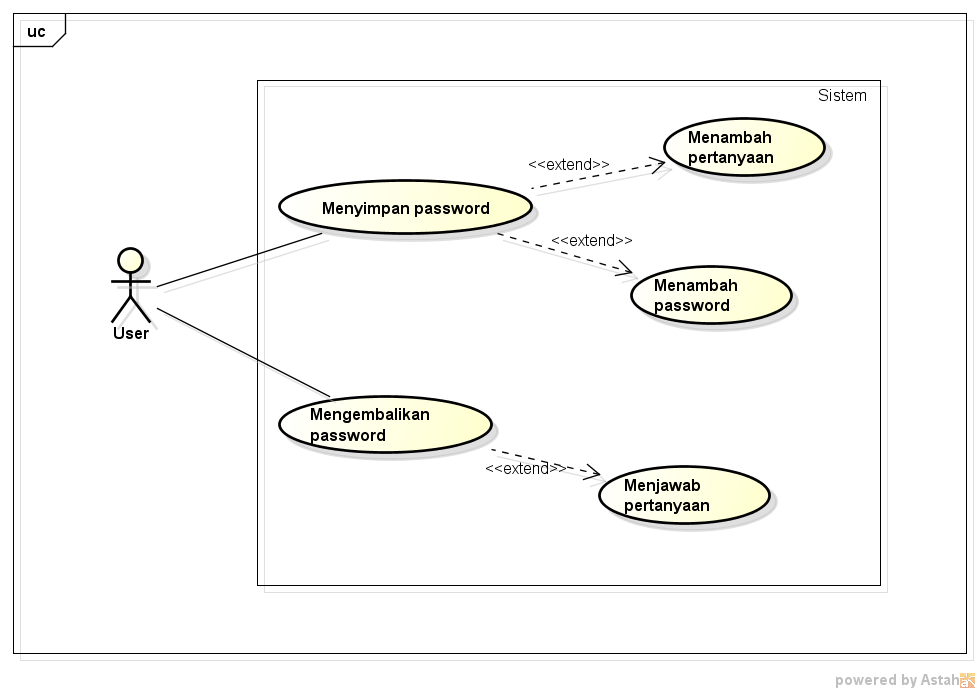
\includegraphics[scale=0.5]{Gambar/use_case}}
	\caption{Diagram \textit{use case} dari perangkat lunak}\label{fig:use_case}
\end{figure}

Adapun skenario-skenario yang pengguna dapat lakukan. Skenario untuk menyimpan \textit{password} ditunjukkan oleh Tabel \ref{table:scenario1}. Aktor dari skenario ini adalah pengguna dari sistem. Data masukan dari skenario ini adalah $n$ \textit{password} dan $n$ pertanyaan keamanan.

\begin{table}[H]
	\centering
	\caption{Skenario Menyimpan \textit{Password}} \label{table:scenario1}
	\begin{tabular}{|l|p{12cm}|}
		\hline
		\textbf{Nama} 					& Menyimpan \textit{Password} 																											\\ \hline
		\textbf{Aktor}					& Pengguna																																					\\ \hline
		\textbf{Deskripsi} 			& Pengguna menyimpan \textit{password} 																							\\ \hline
		\textbf{Kondisi Awal} 	& Aplikasi sudah dijalankan																													\\ \hline
		\textbf{Kondisi Akhir}	& \textit{share} sudah disimpan dalam berkas teks dalam bentuk \textit{ciphertext}	\\ \hline
		\textbf{Skenario Utama} & \begin{enumerate}[itemsep=0mm]\item Pengguna memasukkan \textit{password} dan pertanyaan keamanan \item \textit{Password} dan pertanyaan keamanan diterima oleh sistem\end{enumerate} \\ \hline
		\textbf{Eksepsi}				& Bila masukan tidak valid, sistem akan memberi peringatan \\ \hline
	\end{tabular}
\end{table}

Skenario untuk mengembalikan \textit{password} ditunjukkan oleh Tabel \ref{table:scenario2}. Aktor dari skenario ini adalah pengguna dari sistem. Data masukan dari skenario ini adalah $n$ jawaban dari pertanyaan keamanan yang sudah dibuat.

\begin{table}[H]
	\centering
	\caption{Skenario Mengembalikan \textit{Password}} \label{table:scenario2}
	\begin{tabular}{|l|p{12cm}|}
		\hline
		\textbf{Nama} 					& Mengembalikan \textit{Password} 																									\\ \hline
		\textbf{Aktor}					& Pengguna																																					\\ \hline
		\textbf{Deskripsi} 			& Pengguna mengembalikan \textit{password} 																					\\ \hline
		\textbf{Kondisi Awal} 	& Aplikasi sudah dijalankan	serta \textit{share}, pertanyaan keamanan, dan \textit{salt} sudah disimpan  \\ \hline
		\textbf{Kondisi Akhir}	& Sebanyak $n$ \textit{password} bisa dikembalikan																	\\ \hline
		\textbf{Skenario Utama} & \begin{enumerate}[itemsep=0mm]\item Pengguna menjawab setiap pertanyaan keamanan sebagai masukan \item Masukan diterima oleh sistem \item Sistem memberikan hasil pemrosesan berupa $n$ \textit{password}\end{enumerate} \\ \hline
		\textbf{Eksepsi}				& Bila masukan tidak valid, sistem akan memberi peringatan \\ \hline
	\end{tabular}
\end{table}

\subsection{Diagram Aktivitas}

Perangkat lunak yang dibangun memiliki 2 proses, yaitu menyimpan \textit{password} dan mengembalikan \textit{password}. Urutan aktivitas yang dilakukan perangkat lunak dalam proses menyimpan \textit{password} ditunjukkan pada diagram aktivitas \ref{fig:activity1}.

%diagram
\begin{figure}[H]
	\centerline{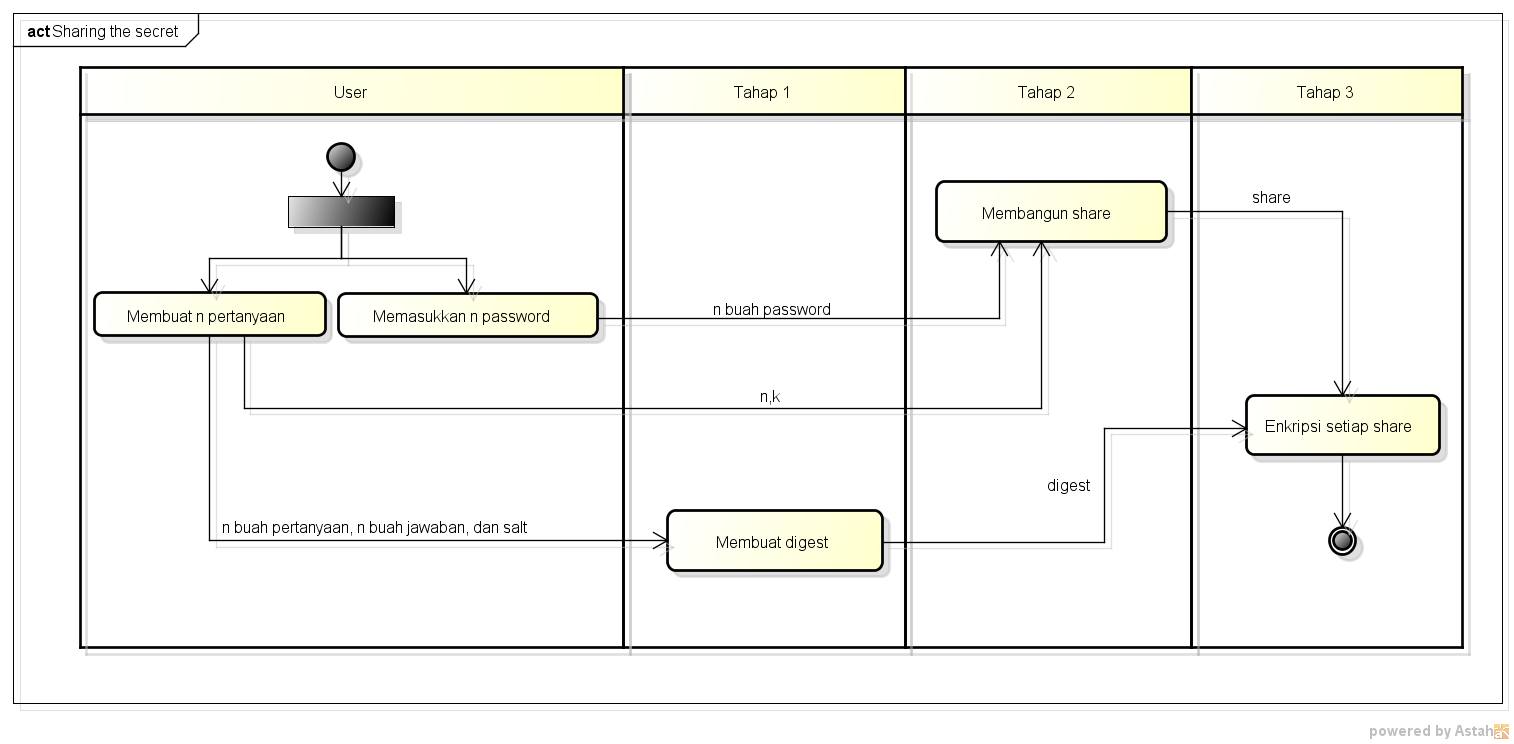
\includegraphics[scale=0.4]{Gambar/sharing-secret}}
	\caption{Diagram aktivitas untuk menyimpan \textit{password}}\label{fig:activity1}
\end{figure}

Dalam proses menyimpan \textit{password}, pengguna memasukkan $n$ \textit{password}. Kemudian, setelah memasukkan $n$ password, pengguna akan membuat $n$ pertanyaan keamanan dan jawaban masing-masing pertanyaan keamanan. Sistem akan menghitung $k$, yaitu minimal banyak pertanyaan yang harus dijawab benar oleh pengguna. Setelah itu, sistem akan memilih secara acak nilai \textit{salt}.

Setelah semua masukan yang dibutuhkan ada, sistem akan membuat \textit{digest} dari konkatenasi setiap pertanyaan keamanan, jawaban, dan nilai \textit{salt}. Sistem juga akan membangun \textit{share} dari masukan \textit{password}. Selanjutnya sistem akan mengenkripsi setiap \textit{share} dari masing-masing \textit{password} dan menggunakan \textit{digest} dari konkatenasi setiap pertanyaan keamanan, jawaban, dan nilai \textit{salt} sebagai kunci proses enkripsi. Setelah proses enkripsi, sistem akan menyimpan seluruh \textit{share} yang sudah dibangun, pertanyaan yang dibuat, $k$, dan nilai \textit{salt}.

Selanjutnya adalah proses mengembalikan \textit{password}. Gambar \ref{fig:activity2} menunjukkan diagram aktivitas untuk proses mengembalikan \textit{password}.

%diagram
\begin{figure}[H]
	\centerline{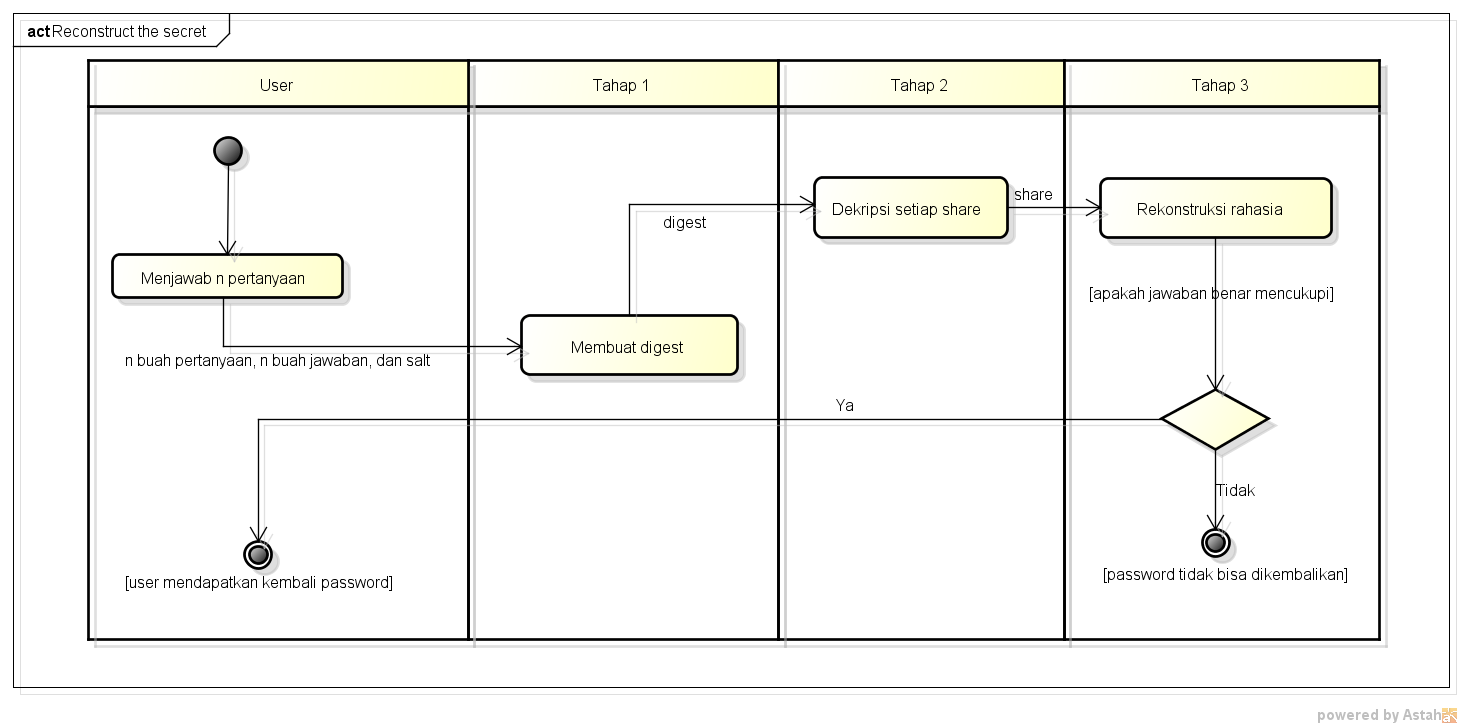
\includegraphics[scale=0.4]{Gambar/reconstruct-secret}}
	\caption{Diagram aktivitas untuk mengembalikan \textit{password}}\label{fig:activity2}
\end{figure}

Dalam proses untuk mengembalikan \textit{password}, pengguna akan diminta untuk menjawab $n$ pertanyaan keamanan yang disimpan saat proses penyimpanan \textit{password}. Sistem akan membuat digest dari konkatenasi setiap pertanyaan keamanan, jawaban pertanyaan keamanan dari masukan pengguna, dan nilai \textit{salt} yang disimpan.

Selanjutnya, sistem akan melakukan proses dekripsi setiap \textit{share} yang sudah disimpan dan menggunakan \textit{digest} sebagai kunci proses dekripsi. Setelah semua \textit{share} didekripsi, sistem akan merekonstruksi \textit{password} dengan \textit{share} dan nilai $k$ yang disimpan sebagai masukan. Jika proses rekonstruksi berhasil, maka pengguna dapat mengembalikan \textit{password}. Sebaliknya, jika proses rekonstruksi gagal, maka \textit{password} tidak bisa dikembalikan.

\subsection{Diagram Kelas}

Pada bagian ini berisi rancangan diagram kelas dari perangkat lunak yang dibangun. Kelas-kelas ini merupakan rancangan kelas yang dibutuhkan untuk membangun perangkat lunak dan dibuat berdasarkan proses-proses yang sudah dijelaskan pada Subbab \ref{sec:analisis}. Rancangan diagram kelas dari perangkat lunak yang dibangun ditunjukkan oleh Gambar \ref{fig:diagramkelasdummy}.

%diagram
\begin{figure}[H]
	\centerline{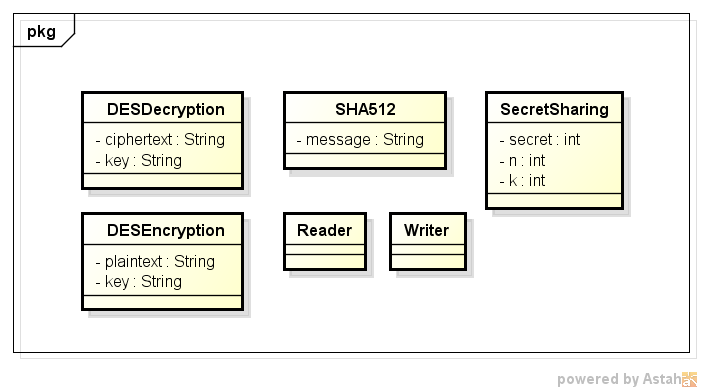
\includegraphics[scale=0.6]{Gambar/engine-class-diagram}}
	\caption{Rancangan Diagram Kelas}\label{fig:diagramkelasdummy}
\end{figure}

Adapun diagram kelas yang ditunjukkan oleh Gambar \ref{fig:diagramkelasdummy} terdiri dari:

\begin{enumerate}
	\item Kelas \textit{DESEncryption} \\
	Kelas \textit{DESEncryption} merupakan kelas yang berperan untuk melakukan proses enkripsi setiap \textit{share}. Kelas ini mengimplementasikan algoritma \textit{Data Encryption Standard} untuk proses enkripsinya.
	\item Kelas \textit{DESDecryption} \\
	Kelas \textit{DESDecryption} merupakan kelas yang berperan untuk melakukan proses dekripsi setiap \textit{share}. Kelas ini mengimplementasikan algoritma \textit{Data Encryption Standard} untuk proses dekripsinya.
	\item Kelas \textit{SHA}512 \\
	Kelas ini berperan untuk membuat \textit{digest} dari konkatenasi masing-masing pertanyaan, jawaban, dan \textit{salt}. Kelas ini mengimplementasikan algoritma \textit{SHA}-512 untuk proses pembuatan \textit{digest}.
	\item Kelas \textit{Secret Sharing} \\
	Kelas ini berperan dalam pembangunan \textit{share}. Kelas ini menggunakan metode \textit{secret sharing} Shamir untuk proses pembangunan \textit{share}.
	\item Kelas Writer \\
	Kelas yang berperan untuk menyimpan setiap keluaran ke dalam berkas teks.
	\item Kelas Reader \\
	Kelas yang berperan untuk membaca berkas teks dan hasil bacaannya akan digunakan sebagai masukan.
\end{enumerate}}{}
\ifdefstring{\vbabd}{1}{\chapter{Perancangan}
\label{chap:perancangan}

Pada bab ini akan dibahas mengenai perancangan perangkat lunak. Perancangan perangkat lunak akan mencakup diagram kelas rinci, perancangan berorientasi objek, dan perancangan antarmuka.

\section{Diagram Kelas Rinci}

Diagram kelas rinci digunakan sebagai gambaran umum untuk setiap kelas yang ada dalam perangkat lunak yang dibangun serta keterkaitan setiap kelas. Diagram kelas rinci dapat dilihat pada Gambar \ref{fig:final_class_diagram}. Ada perbedaan antara diagram kelas pada Gambar \ref{fig:final_class_diagram} dengan kelas diagram pada Bab \ref{chap:analisis}. Pada diagram kelas rinci ditambahkan beberapa atribut dan fungsi sesuai dengan kebutuhan dari masing-masing kelas.

%\clearpage
%diagram
%\begin{sidewaysfigure}[H]
	%\centerline{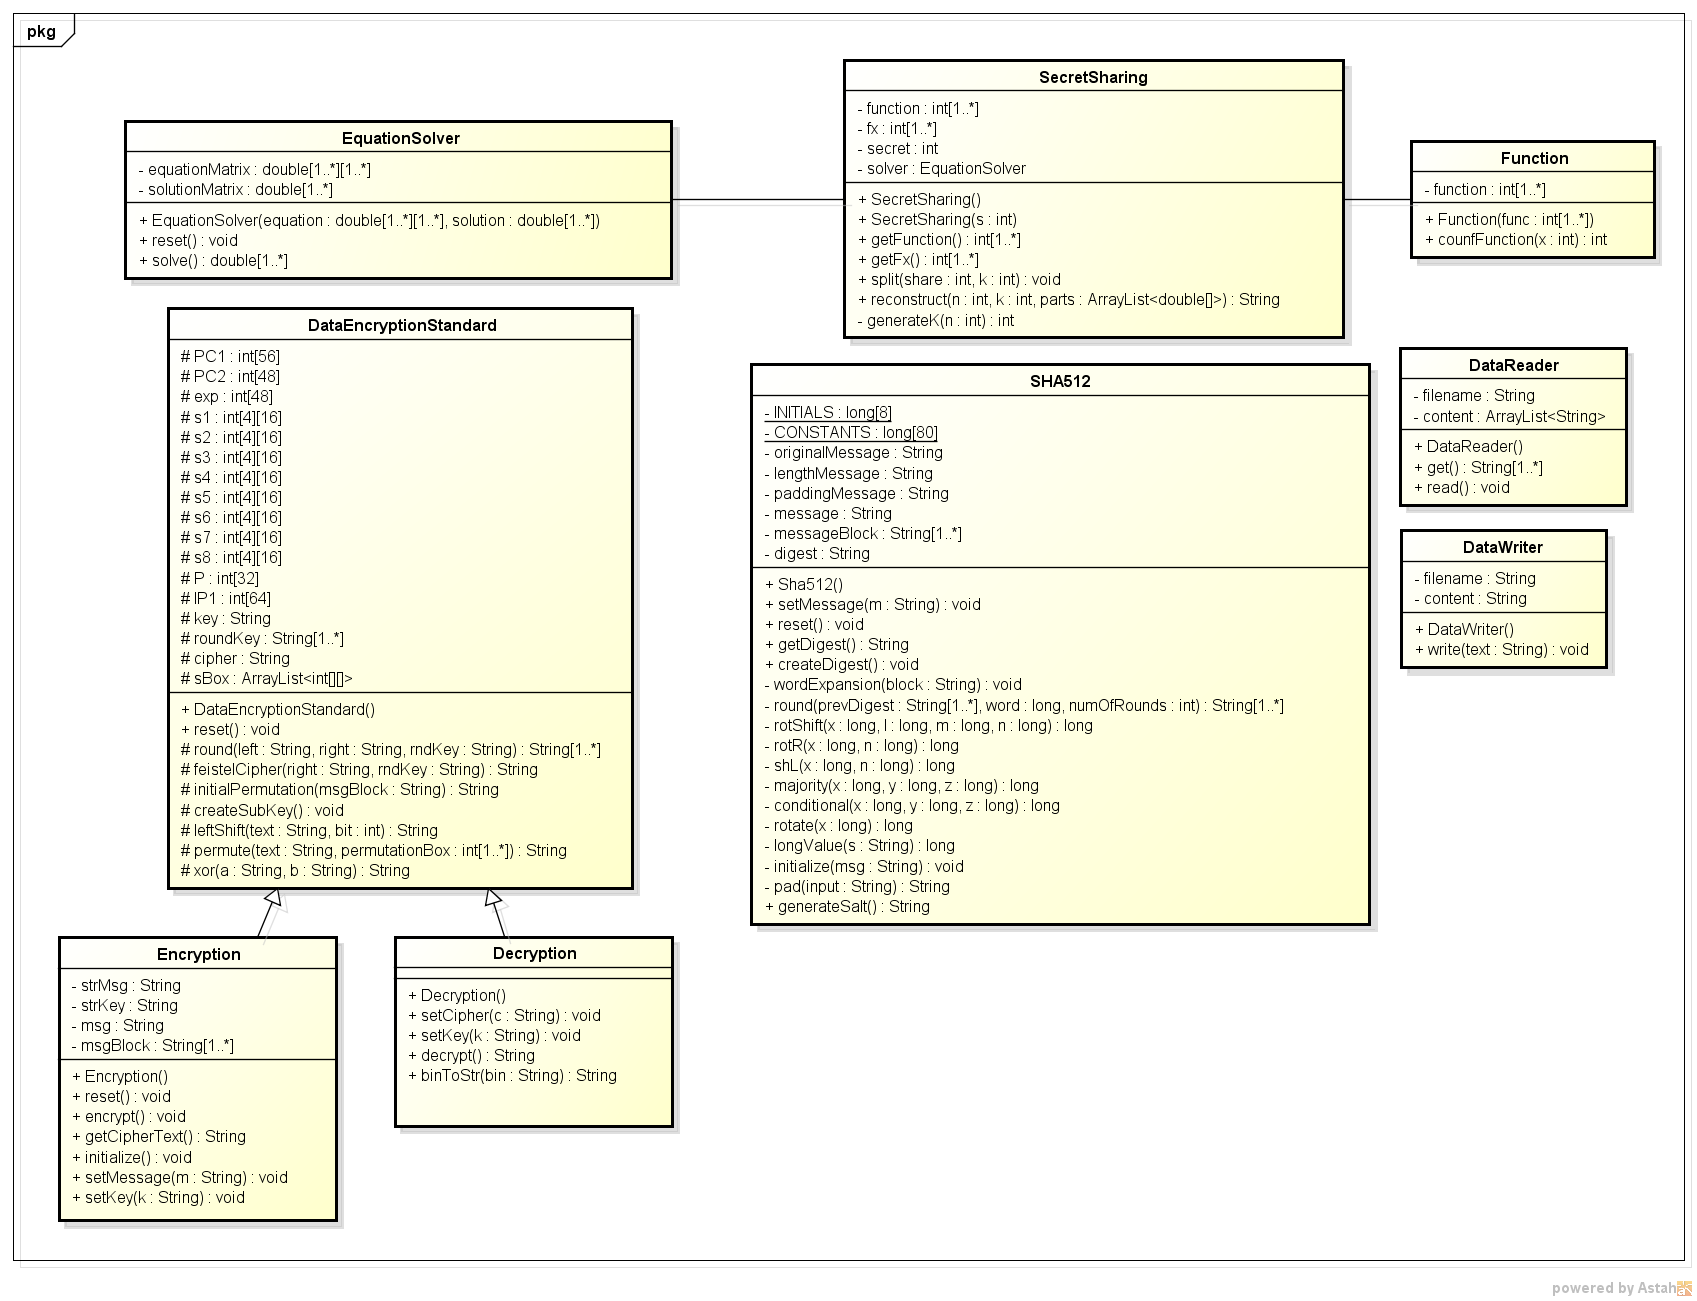
\includegraphics[scale=0.5]{Gambar/final_class_diagram}}
	%\caption{Diagram Kelas Rinci}\label{fig:final_class_diagram}
%\end{sidewaysfigure}

\begin{figure}[h]
	\centering
	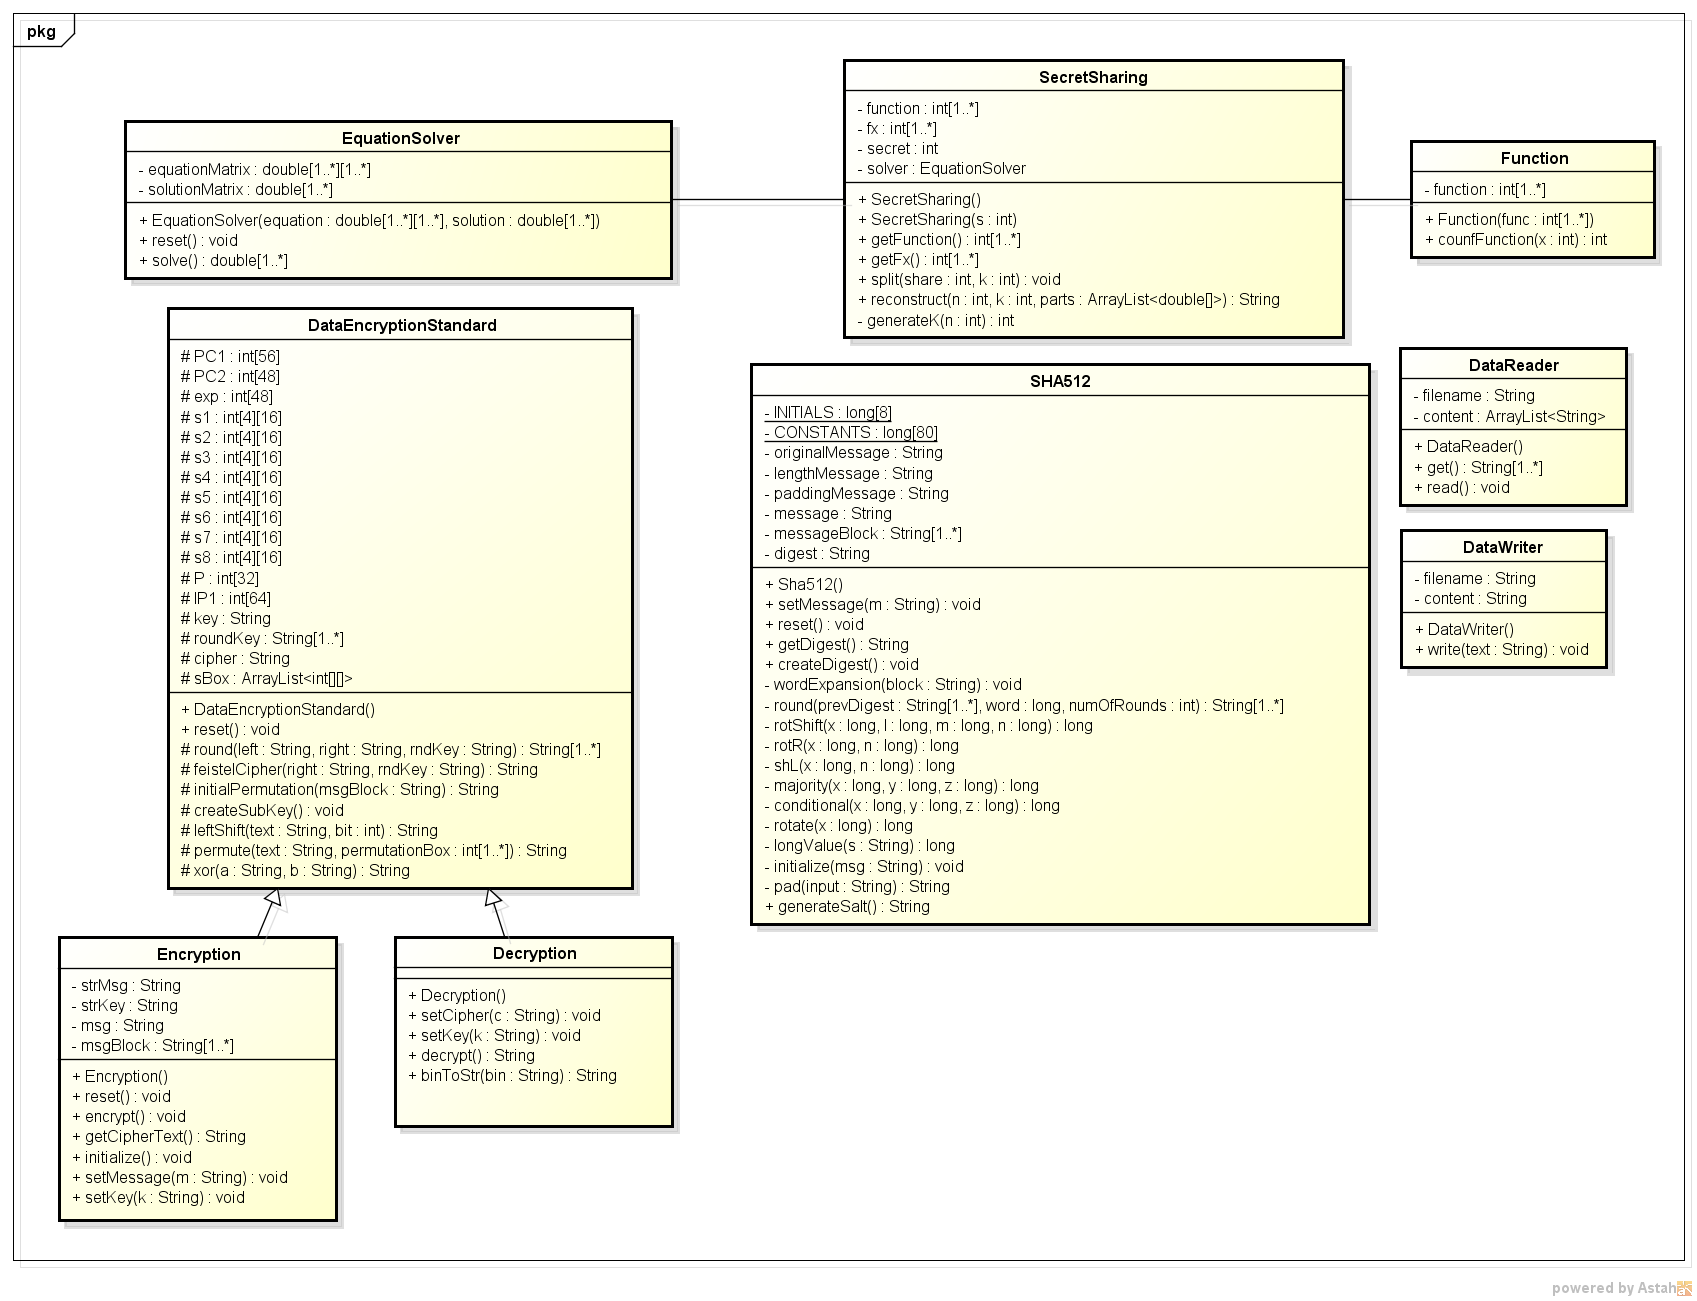
\includegraphics[angle=90, origin=c, scale=0.5]{Gambar/final_class_diagram}
	\caption{Diagram Kelas Rinci}\label{fig:final_class_diagram}
\end{figure}

\section{Deskripsi Kelas dan Fungsi}

Pada bagian ini akan berisi mengenai penjelasan secara rinci masing-masing kelas. Tujuannya adalah menjelaskan peran setiap kelas dalam perangkat lunak yang dibangun.

\subsection{Kelas \textit{SHA512}}

Kelas \textit{SHA512} merupakan kelas yang mengimplementasikan \textit{Secure Hashing Algorithm 512} (SHA-512). Cara kerja algoritma dapat dilihat pada bagian \ref{sec:SHA512}. Struktur kelas \textit{SHA512} ditunjukkan pada Gambar \ref{fig:classsha512}.

\begin{figure}[H]
	\centering
	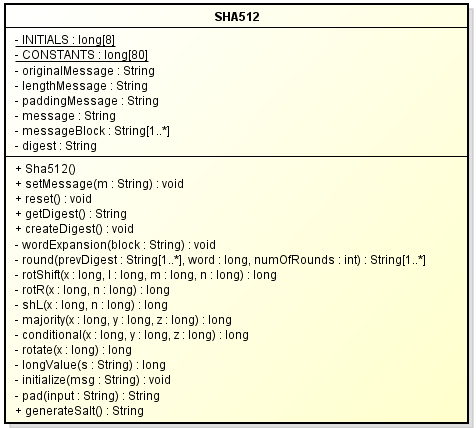
\includegraphics[scale=0.5]{Gambar/class_sha512}
	\caption{Kelas SHA512}\label{fig:classsha512}
\end{figure}

Adapun atribut dari kelas \textit{SHA512}, yaitu \textit{INITIALS, CONSTANTS, originalMessage, lengthMessage, paddingMessage, message, messageBlock,} dan \textit{digest}. Berikut penjelasan masing-masing atribut tersebut:

\begin{enumerate}
	\item \textit{long[8] INITIALS} \\
	Atribut yang berguna untuk menyimpan nilai dari konstanta awal.
	\item \textit{long[80] INITIALS} \\
	Atribut yang berguna untuk menyimpan konstanta yang digunakan dalam setiap putaran SHA-512.
	\item \textit{String originalMessage} \\
	Atribut yang berguna untuk menyimpan \textit{message} yang belum di\textit{padding} dalam bentuk \textit{string} biner.
	\item \textit{String lengthMessage} \\
	Atribut yang berguna untuk menyimpan informasi mengenai panjang atribut \textit{originalMessage} dalam bentuk \textit{string} biner.
	\item \textit{String paddingMessage} \\
	Atribut yang berguna untuk menyimpan blok \textit{padding} dalam bentuk \textit{string} biner.
	\item \textit{String message} \\
	Atribut yang berguna untuk menyimpan \textit{message} yang sudah di\textit{padding} dalam bentuk \textit{string} biner.
	\item String digest \\
	Atribut yang berguna untuk menyimpan \textit{digest} dari atribut \textit{message} dalam bentuk string \textit{biner}.
\end{enumerate}

Adapun fungsi yang membangun kelas \textit{SHA512}, yaitu \textit{Sha512, setMessage, reset, getDigest, wordExpansion, round, rotShift, rotR, shL, majority, conditional, rotate, longValue, initialize, pad} dan \textit{generateSalt}. Berikut penjelasan masing-masing fungsi tersebut:

\begin{enumerate}
	\item \textit{Sha512} \\
	Merupakan konstruktor dari kelas \textit{SHA512}.
	\item \textit{void setMessage(String m)} \\
	Fungsi yang berguna untuk menyimpan nilai \textit{string m} ke dalam atribut \textit{originalMessage}.
	\item \textit{void reset} \\
	Fungsi yang berguna untuk mengembalikan nilai atribut \textit{originalMessage, lengthMessage, paddingMessage, message,} dan \textit{digest} menjadi \textit{string} kosong dan mengembalikan nilai atribut \textit{messageBlock} menjadi \textit{array string} kosong.
	\item \textit{String getDigest} \\
	Fungsi yang berguna untuk mengembalikan nilai atribut \textit{digest} dalam bentuk heksadesimal.
	\item \textit{void createDigest} \\
	Fungsi yang berperan untuk membuat \textit{digest} dari \textit{message}. Algoritma untuk membuat \textit{digest} ini dapat dilihat pada bagian \ref{sec:SHA512}.
	\item \textit{void wordExpansion(String block)} \\
	Fungsi yang berperan untuk melakukan proses ekspansi blok \textit{message}.
	\item \textit{String[] round(String[] prevDigest, long word, int numOfRounds)} \\
	Fungsi yang berperan untuk melakukan 1 putaran dari \textit{SHA512}. Proses yang terjadi dalam 1 putaran \textit{SHA512} dapat dilihat pada Bab \ref{sec:SHA512}.
	\item \textit{long rotShift(long x, long m, long n)} \\
	Fungsi yang berperan untuk melakukan operasi \begin{math}RotShift_{l-m-n}(x)\end{math} (Subbab \ref{subsec:expansiblokmsg}).
	\item \textit{long rotR(long x, long n)} \\
	Fungsi yang berperan untuk melakukan operasi \begin{math}RotR_i(x)\end{math} (Subbab \ref{subsec:expansiblokmsg}).
	\item \textit{long shL(long x, long n)} \\
	Fungsi yang berperan untuk melakukan operasi \begin{math}ShL_i(x)\end{math} (Subbab \ref{subsec:expansiblokmsg}).
	\item \textit{long majority(long x, long y, long z)} \\
	Fungsi yang berperan untuk melakukan operasi \begin{math}Majority(x,y,z)\end{math} (Subbab \ref{subsec:putaransha}).
	\item \textit{long conditional(long x, long y, long z)} \\
	Fungsi yang berperan untuk melakukan operasi \begin{math}Conditional(x,y,z)\end{math} (Subbab \ref{subsec:putaransha}).
	\item \textit{long rotate(long x)} \\
	Fungsi yang berperan untuk melakukan operasi \begin{math}Rotate(x)\end{math} (Subbab \ref{subsec:putaransha}).
	\item \textit{long longValue(String s)} \\
	Fungsi yang berperan mengubah tipe data \textit{string s} menjadi tipe data \textit{long}.
	\item \textit{void initialize(String msg)} \\
	Fungsi yang berperan untuk melakukan proses \textit{message padding} dan memecah menjadi blok-blok \textit{message}.
	\item \textit{String pad(String input)} \\
	Fungsi yang berperan untuk menambahkan \textit{padding} angka 0 pada \textit{string} biner \textit{input}. Algoritma fungsi ini ditunjukkan pada Algoritma \ref{padString}.
	
	\begin{algorithm}[H]
		\caption{pad}
		\label{padString}
		\begin{algorithmic}[1]
			\Function{pad}{input}
				\If{\begin{math}input.length \: mod\: 8 != 0\end{math}}
					\State \begin{math}add = 8 - (input.length \: mod\: 8)\end{math}
				\EndIf
				\For{$i < add$}
					\State $res = res + "0"$
				\EndFor
				\State $res = res + input$
				\State \Return $res$
			\EndFunction
		\end{algorithmic}
	\end{algorithm}
	
	\item \textit{String generateSalt} \\
	Fungsi yang berguna untuk membangun nilai \textit{salt}. Nilai \textit{salt} yang dibangun terdiri dari 4 karakter ASCII acak. Algoritma fungsi ini ditunjukkan pada Algoritma \ref{salting}.
	\begin{algorithm}[H]
		\caption{generateSalt}
		\label{salting}
		\begin{algorithmic}[1]
			\Function{generateSalt}{}
			  \State $i = 0$
				\For{$i < 4$}
					\State $temp = random((126-33) + 1) + 33$
					\State $salt += temp.toString$
				\EndFor
				\State \Return $salt$
			\EndFunction
		\end{algorithmic}
	\end{algorithm}
\end{enumerate}

\subsection{Kelas \textit{Function}}

Kelas \textit{Function} merupakan kelas yang merepresentasikan sebuah fungsi polinomial \begin{math}f(x)\end{math}. Kelas \textit{Function} ditunjukkan pada Gambar \ref{fig:classfunction}.

\begin{figure}[H]
	\centering
	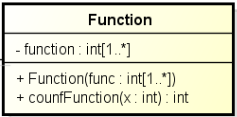
\includegraphics[scale=0.7]{Gambar/class_function}
	\caption{Kelas \textit{Function}}\label{fig:classfunction}
\end{figure}

Adapun atribut dari kelas \textit{Function} adalah \textit{function}. Atribut \textit{function} berguna untuk menyimpan nilai setiap koefesien dari fungsi polinomial \begin{math}f(x)\end{math} dalam tipe data \textit{array} bilangan bulat.

Sementara itu, fungsi yang dimiliki oleh kelas \textit{Function}, yaitu \textit{Function} dan \textit{countFunction}. Berikut penjelasan masing-masing fungsi:

\begin{enumerate}
	\item \textit{Function(int[] func)} \\
	Merupakan konstruktor dari kelas \textit{Function} yang menerima masukan \textit{array} bilangan bulat.
	\item \textit{int countFunction(int x)} \\
	Menghitung nilai \begin{math}x\end{math} untuk fungsi polinomial \begin{math}f(x)\end{math}. Algoritma dari fungsi ini ditunjukkan pada Algoritma \ref{countFunction}.
	\begin{algorithm}[H]
		\caption{countFunction}
		\label{countFunction}
		\begin{algorithmic}[1]
			\Function{countFunction}{x}
				\For{$i < function.length$}
					\State \begin{math}res = res + (function[i]\: \cdot\: x^i)\end{math}
				\EndFor
				\State \Return \begin{math}res\end{math}
			\EndFunction
		\end{algorithmic}
	\end{algorithm}
\end{enumerate}

\subsection{Kelas \textit{EquationSolver}}

Kelas \textit{EquationSolver} adalah kelas yang mengimplementasikan eliminasi Gauss-Jordan (Bagian \ref{sec:eliminasigaussjordan}). Kelas ini berperan untuk menyelesaikan persamaan linear. Gambar \ref{fig:classequationsolver} menunjukkan struktur dari kelas \textit{EquationSolver}.

\begin{figure}[H]
	\centering
	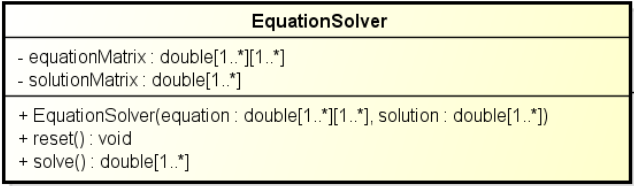
\includegraphics[scale=0.7]{Gambar/class_equation_solver}
	\caption{Kelas \textit{EquationSolver}}\label{fig:classequationsolver}
\end{figure}

Adapun atribut dari kelas \textit{EquationSolver}, yaitu \textit{equationMatrix} dan \textit{solutionMatrix}. Berikut penjelasan masing-masing atribut:

\begin{enumerate}
	\item \textit{double[][] equationMatrix} \\
	Atribut yang menyimpan bentuk matriks dari persamaan linear.
	\item \textit{double[] solutionMatrix} \\
	Atribut yang menyimpan bentuk matriks dari solusi masing-masing persamaan linear.
\end{enumerate}

Sementara itu, fungsi yang dimiliki oleh kelas \textit{EquationSolver}, yaitu \textit{EquationSolver}, \textit{reset}, dan \textit{solve}. Berikut penjelasan masing-masing fungsi:

\begin{enumerate}
	\item \textit{EquationSolver(double[][] equation, double[] solution)} \\
	Merupakan konstruktor dari kelas \textit{EquationSolver} yang menerima masukan berupa matriks persamaan dan matriks solusi.
	\item \textit{void reset} \\
	Mengembalikan nilai atribut \textit{equationMatrix} dan \textit{solutionMatrix} menjadi \textit{array} kosong.
	\item double[] solve \\
	Mencari solusi dari persamaan linear dan mengembalikan solusi dalam bentuk \textit{array}.
\end{enumerate}

\subsection{Kelas \textit{SecretSharing}}

Kelas \textit{SecretSharing} adalah kelas yang mengimplementasikan skema \textit{threshold(k,n)}. Kelas ini berperan untuk membangun \textit{share} dan juga merekonstruksi rahasia dari \textit{share}. Struktur kelas \textit{SecretSharing} ditunjukkan oleh Gambar \ref{fig:classsecretsharing}.

\begin{figure}[H]
	\centering
	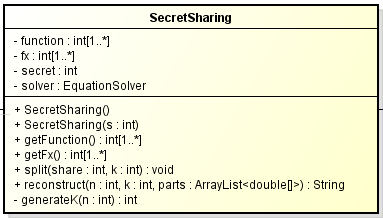
\includegraphics[scale=0.7]{Gambar/class_secret_sharing}
	\caption{Kelas \textit{DESEncryption}}\label{fig:classdesencryption}
\end{figure}

Kelas \textit{SecretSharing} memiliki beberapa atribut, yaitu \textit{function, fx, secret,} dan \textit{solver}. Berikut penjelasan masing-masing atribut:

\begin{enumerate}
	\item \textit{int[] function} \\
	Atribut yang menyimpan nilai setiap koefesien dari fungsi polinomial \begin{math}f(x)\end{math} dalam tipe data \textit{array} bilangan bulat.
	\item \textit{int[] fx} \\
	Atribut yang menyimpan nilai setiap koefesien dari rumus dasar fungsi \begin{math}f(x)\end{math} dalam tipe data \textit{array} bilangan bulat.
	\item \textit{int secret} \\
	Atribut yang menyimpan rahasia yang akan dibangun \textit{share-share}nya.
	\item \textit{EquationSolver solver} \\
	Atribut dari objek kelas \textit{EquationSolver}.
\end{enumerate}

Kelas \textit{SecretSharing} memiliki beberapa fungsi, yaitu \textit{SecretSharing, SecretSharing(int s), getFunction, getFx, split, reconstruct} dan \textit{generateK}. Berikut penjelasan masing-masing fungsi:

\begin{enumerate}
	\item \textit{SecretSharing} \\
	Merupakan konstruktor kosong dari kelas \textit{SecretSharing}.
	\item \textit{SecretSharing(int s)} \\
	Merupakan konstruktor dengan masukan \textit{int s} yang akan disimpan ke dalam atribut \textit{secret}.
	\item \textit{int[] getFunction} \\
	Fungsi yang berguna untuk mengembalikan nilai atribut \textit{function}.
	\item \textit{int[] getFx} \\
	Fungsi yang berguna untuk mengembalikan nilai atribut \textit{fx}.
	\item \textit{split(int share, int k)} \\
	Fungsi yang berperan dalam proses pembangunan \textit{share-share}. Cara pembangunan \textit{share} dapat dilihat pada Bab \ref{sec:secretsharingshamir}.
	\item \textit{String reconstruct(int n, int k, ArrayList<double[]> parts)} \\
	Fungsi yang berperan dalam proses rekonstruksi rahasia dari \textit{share-share} yang dimiliki. \textit{Share-share} yang dimiliki ini disimpan dalam masukan \textit{ArrayList<double[]> parts}. Proses rekonstruksi rahasia dapat dilihat pada Bab \ref{sec:secretsharingshamir}.
	\item \textit{int generateK(int n)} \\
	Fungsi ini berperan untuk menentukan nilai $k$ yang ideal berdasarkan nilai $n$. Algoritma untuk menentukan nilai $k$ ditunjukkan oleh Algoritma \ref{generateK}.
	\begin{algorithm}[H]
		\caption{generateK}
		\label{generateK}
		\begin{algorithmic}[1]
			\Function{generateK}{n}
				\State $k = n/2 + 1$
				\If{$k > n$}
					\State $k = n$
				\EndIf
				\State \Return \begin{math}k\end{math}
			\EndFunction
		\end{algorithmic}
	\end{algorithm}
\end{enumerate}

\subsection{Kelas \textit{DataEncryptionStandard}}

Kelas \textit{DataEncryptionStandard} merupakan kelas yang mengimplementasikan algoritma \textit{Data Encryption Standard} (DES). Kelas ini akan menjadi kelas \textit{parent} dari proses enkripsi dan dekripsi. Struktur kelas \textit{DataEncryptionStandard} ditunjukkan oleh Gambar \ref{fig:classdes}.

\begin{figure}[H]
	\centering
	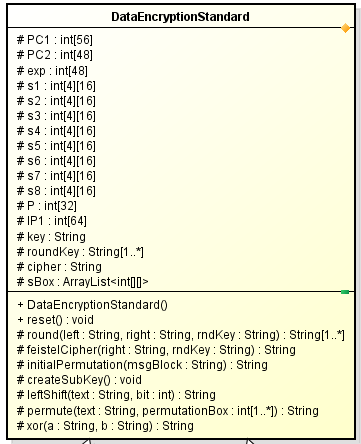
\includegraphics[scale=0.6]{Gambar/class_des}
	\caption{Kelas \textit{DataEncryptionStandard}}\label{fig:classdes}
\end{figure}

Kelas Encryption memiliki beberapa atribut, yaitu \textit{PC1, PC2, IP, exp, s1, s2, s3, s4, s5, s6, s7, s8, P, IP1, key, roundKey, cipher,} dan \textit{sBox}. Berikut penjelasan masing-masing atribut:

\begin{enumerate}
	\item \textit{int[56] PC1} \\
	Atribut yang menyimpan matriks \textit{parity drop} yang digunakan dalam proses pembangkitan kunci putaran.
	\item \textit{int[48] PC2} \\
	Atribut yang menyimpan matriks permutasi \textit{P-box} yang digunakan dalam proses pembangkitan kunci putaran.
	\item \textit{int[64] IP} \\
	Atribut yang menyimpan matriks permutasi awal.
	\item \textit{int[48] exp} \\
	Atribut yang menyimpan matriks ekspansi \textit{P-box}.
	\item \textit{int[4][16] s1} \\
	Atribut yang menyimpan matriks \textit{s-box} ke-1.
	\item \textit{int[4][16] s2} \\
	Atribut yang menyimpan matriks \textit{s-box} ke-2.
	\item \textit{int[4][16] s3} \\
	Atribut yang menyimpan matriks \textit{s-box} ke-3.
	\item \textit{int[4][16] s4} \\
	Atribut yang menyimpan matriks \textit{s-box} ke-4.
	\item \textit{int[4][16] s5} \\
	Atribut yang menyimpan matriks \textit{s-box} ke-5.
	\item \textit{int[4][16] s6} \\
	Atribut yang menyimpan matriks \textit{s-box} ke-6.
	\item \textit{int[4][16] s7} \\
	Atribut yang menyimpan matriks \textit{s-box} ke-7.
	\item \textit{int[4][16] s8} \\
	Atribut yang menyimpan matriks \textit{s-box} ke-8.
	\item \textit{int[32] P} \\
	Atribut yang menyimpan matriks permutasi pada tahap terakhir fungsi DES.
	\item \textit{int[64] IP1} \\
	Atribut yang menyimpan matriks permutasi akhir.
	\item \textit{String key} \\
	Atribut yang menyimpan kunci dalam bentuk \textit{string} biner.
	\item \textit{String[] roundKey} \\
	Atribut yang menyimpan kunci untuk setiap putaran dalam \textit{array string} biner.
	\item \textit{String cipher} \\
	Atribut yang menyimpan \textit{ciphertext} hasil enkripsi dalam bentuk \textit{string} biner.
	\item \textit{ArrayList<int[][]> sBox} \\
	Atribut yang menyimpan seluruh matriks \textit{s-box}.
\end{enumerate}

Adapun fungsi-fungsi yang dimiliki oleh kelas \textit{DataEncryptionStandard}, yaitu \textit{DataEncryptionStandard, reset, round, feistelCipher, initialPermutation, createSubKey, leftShift, permute,} dan \textit{xor}. Berikut penjelasan masing-masing fungsi:

\begin{enumerate}
	\item \textit{DataEncryptionStandard} \\
	Merupakan konstruktor dari kelas \textit{DataEncryptionStandard}.
	\item \textit{void reset} \\
	Fungsi yang berperan untuk mengembalikan atribut \textit{key} dan \textit{cipher} menjadi \textit{string} kosong. Fungsi ini juga mengembalikan atribut \textit{roundKey} menjadi \textit{array string} kosong.
	\item \textit{String[] round(String left, String right, String rndKey)} \\
	Fungsi yang berperan untuk melakukan 1 putaran dari DES. Fungsi ini mengembalikan \textit{array string} yang berguna untuk blok masukan putaran berikutnya.
	\item \textit{String feistelCipher(String right, String rndKey)} \\
	Fungsi yang berperan untuk melakukan proses jaringan Feistel kepada blok bagian kanan dari \textit{plaintext}.
	\item \textit{String initialPermutation(String msgBlock)} \\
	Fungsi ini berperan untuk melakukan proses permutasi awal.
	\item \textit{void createSubKey} \\
	Fungsi yang berperan untuk membangkitkan kunci putaran.
	\item \textit{String leftShift(String text, int bit)} \\
	Fungsi yang berperan untuk melakukan \textit{shift left} dari masukan \textit{string text} sebanyak masukan \textit{int bit}.
	\item \textit{String permute(String text, int[] permutationBox)} \\
	Fungsi yang berperan untuk melakukan proses permutasi.
	\item \textit{String xor(String a, String b)} \\
	Fungsi yang berperan untuk melakukan operasi XOR.
\end{enumerate}

\subsection{Kelas \textit{Encryption}}

Kelas \textit{Encryption} merupakan kelas turunan dari kelas \textit{DataEncryptionStandard}. Kelas ini berperan untuk melakukan proses enkripsi menggunakan algoritma \textit{Data Encryption Standard}. Struktur kelas \textit{Encryption} ditunjukkan oleh Gambar \ref{fig:classdesencryption}.

\begin{figure}[H]
	\centering
	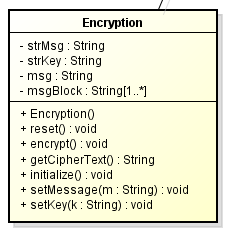
\includegraphics[scale=0.6]{Gambar/class_des_encryption}
	\caption{Kelas \textit{Encryption}}\label{fig:classdesencryption}
\end{figure}

Kelas Encryption memiliki beberapa atribut, yaitu \textit{strMsg, strKey, msg,} dan \textit{msgBlock}. Berikut penjelasan masing-masing atribut:

\begin{enumerate}
	\item \textit{String strMsg} \\
	Atribut yang menyimpan \textit{plaintext} dalam bentuk \textit{string}.
	\item \textit{String strKey} \\
	Atribut yang menyimpan kunci dalam bentuk \textit{string}.
	\item \textit{String msg} \\
	Atribut yang menyimpan \textit{plaintext} dalam bentuk \textit{string} biner.
	\item \textit{String[] msgBlock} \\
	Atribut yang menyimpan blok-blok \textit{plaintext} dalam bentuk \textit{array string} biner. Setiap elemen \textit{array} berisi \textit{string} biner dengan panjang 64-\textit{bit}.
\end{enumerate}

Adapun fungsi-fungsi yang dimiliki oleh kelas \textit{Encryption}, yaitu \textit{Encryption, reset, encrypt, getCipherText, initialize, setMessage,} dan \textit{setKey}. Berikut penjelasan masing-masing fungsi:

\begin{enumerate}
	\item \textit{Encryption} \\
	Merupakan konstruktor dari kelas \textit{Encryption}.
	\item \textit{void reset} \\
	Fungsi yang berperan untuk mengembalikan atribut \textit{strMsg, strKey, msg, key,} dan \textit{cipher} menjadi \textit{string} kosong. Fungsi ini juga mengembalikan atribut \textit{roundKey} dan \textit{msgBlock} menjadi \textit{array string} kosong.
	\item \textit{void encrypt} \\
	Fungsi yang berperan untuk melakukan proses enkripsi DES.
	\item \textit{String getCipherText} \\
	Fungsi yang mengembalikan nilai atribut \textit{cipher} dalam bentuk \textit{string} heksadesimal.
	\item \textit{void setMessage(String m)} \\
	Fungsi untuk menyimpan \textit{string m} ke dalam atribut \textit{strMsg}.
	\item \textit{void setKey(String k)} \\
	Fungsi untuk menyimpan \textit{string k} ke dalam atribut \textit{strKey}.
	\item \textit{void initialize} \\
	Fungsi yang berperan untuk melakukan \textit{padding} terhadap \textit{strMsg} dan memecah \textit{strMsg} menjadi blok-blok \textit{string}. Blok-blok \textit{string} ini akan disimpan pada atribut \textit{msgBlock}.
\end{enumerate}

\subsection{Kelas \textit{Decryption}}

Kelas \textit{Decryption} merupakan kelas turunan dari kelas \textit{DataEncryptionStandard}. Kelas ini berperan untuk melakukan proses dekripsi menggunakan algoritma \textit{Data Encryption Standard}. Struktur kelas \textit{Decryption} ditunjukkan pada Gambar \ref{fig:classdesdecryption}.

\begin{figure}[H]
	\centering
	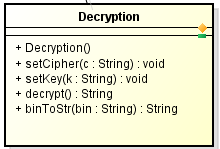
\includegraphics[scale=0.6]{Gambar/class_des_decryption}
	\caption{Kelas \textit{DESDecryption}}\label{fig:classdesdecryption}
\end{figure}

Kelas \textit{Decryption} tidak memiliki atribut. Seluruh atribut dari kelas ini diturunkan dari kelas \textit{DataEncryptionStandard}. Adapun fungsi-fungsi yang dimiliki kelas \textit{Decryption}, yaitu \textit{Decryption, setCipher, setKey, decrypt,} dan \textit{binToStr}. Berikut penjelasan masing-masing fungsi:

\begin{enumerate}
	\item \textit{Decryption} \\
	Merupakan konstruktor dari kelas \textit{Decryption}.
	\item \textit{void setCipher(String c)} \\
	Fungsi untuk menyimpan \textit{string c} pada atribut \textit{cipher} dalam bentuk \textit{string} biner.
	\item \textit{void setKey(String k)} \\
	Fungsi untuk menyimpan \textit{string k} pada atribut \textit{key} dalam bentuk \textit{string} biner.
	\item \textit{String decrypt} \\
	Fungsi yang berperan untuk melakukan proses dekripsi menggunakan DES.
	\item \textit{String binToStr(String bin)} \\
	Fungsi yang berperan untuk mengubah \textit{string} biner menjadi \textit{string}.
\end{enumerate}

\subsection{Kelas \textit{DataReader}}

Kelas \textit{DataReader} merupakan kelas yang berperan untuk membaca berkas teks. Kelas \textit{DataReader} ditunjukkan pada Gambar \ref{fig:classdatareader}.

\begin{figure}[H]
	\centering
	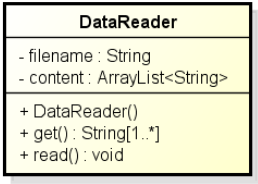
\includegraphics[scale=0.8]{Gambar/class_data_reader}
	\caption{Kelas \textit{DataReader}}\label{fig:classdatareader}
\end{figure}

Kelas ini memiliki 2 atribut, yaitu \textit{filename} dan \textit{content}. Berikut penjelasan masing-masing atribut:

\begin{enumerate}
	\item \textit{String filename} \\
	Atribut yang menyimpan nama dari berkas teks yang dibaca.
	\item \textit{ArrayList<String> content} \\
	Atribut yang menyimpan isi dari berkas teks yang dibaca.
\end{enumerate}

Adapun kelas ini memiliki 3 fungsi, yaitu \textit{DataReader, get,} dan \textit{read}. Berikut penjelasan masing-masing fungsi:

\begin{enumerate}
	\item \textit{DataReader} \\
	Merupakan konstruktor dari kelas \textit{DataReader}.
	\item \textit{String[] get} \\
	Fungsi yang berguna untuk mengembalikan atribut \textit{content}.
	\item \textit{void read} \\
	Fungsi yang berperan membaca berkas teks.
\end{enumerate}

\subsection{Kelas \textit{DataWriter}}

Kelas \textit{DataWriter} adalah kelas yang berperan untuk menulis keluaran ke dalam berkas teks. Kelas \textit{DataWriter} ditunjukkan pada Gambar \ref{fig:classdatawriter}.

\begin{figure}[H]
	\centering
	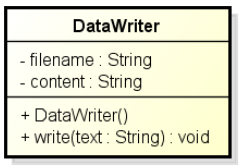
\includegraphics[scale=0.8]{Gambar/class_data_writer}
	\caption{Kelas \textit{DataWriter}}\label{fig:classdatawriter}
\end{figure}

Kelas ini memiliki 2 atribut, yaitu \textit{filename} dan \textit{content}. Berikut penjelasan masing-masing atribut:

\begin{enumerate}
	\item \textit{String filename} \\
	Atribut yang menyimpan nama dari berkas teks yang akan ditulis.
	\item \textit{String content} \\
	Atribut yang menyimpan isi dari berkas teks yang akan ditulis.
\end{enumerate}

Adapun kelas ini memiliki 2 fungsi, yaitu DataWriter dan write. Berikut penjelasan masing-masing fungsi:

\begin{enumerate}
	\item DataWriter \\
	Merupakan konstruktor dari kelas \textit{DataWriter}.
	\item \textit{write(String text)} \\
	Fungsi yang berperan untuk menulis isi dari berkas teks.
\end{enumerate}

\section{Perancangan Antarmuka}

Perangkat lunak yang dikembangkan akan memiliki 3 tampilan utama, tampilan untuk menyimpan \textit{password}, tampilan untuk mengembalikan \textit{password}, dan tampilan untuk memilih menyimpan \textit{password} atau mengembalikan \textit{password}.

Gambar \ref{fig:tampilan-awal} menunjukkan tampilan awal yang akan dimunculkan pertama kali untuk memilih menyimpan \textit{password} atau mengembalikan \textit{password}.

%diagram
\begin{figure}[H]
	\centerline{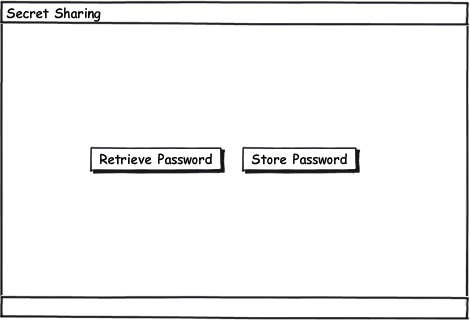
\includegraphics[scale=0.5]{Gambar/tampilan-utama}}
	\caption{Perancangan Tampilan Awal}\label{fig:tampilan-awal}
\end{figure}

Tampilan utama ini cukup sederhana. Dalam tampilan utama pada Gambar \ref{fig:tampilan-awal}, hanya terdapat 2 pilihan, yaitu \textit{store password} untuk menyimpan \textit{password} dan \textit{retrieve password} untuk mengembalikan \textit{password}. Selanjutnya, jika pengguna memilih \textit{store password}, maka akan ditampilkan halaman \textit{store password}.

%diagram
\begin{figure}[H]
	\centerline{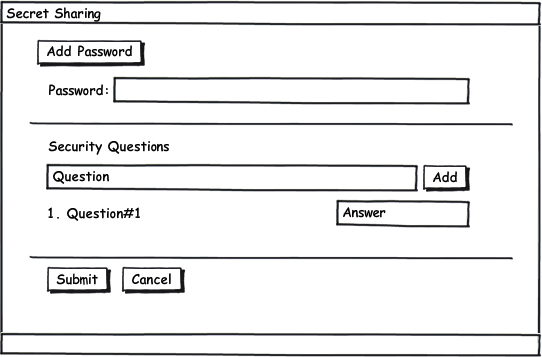
\includegraphics[scale=0.5]{Gambar/store_password}}
	\caption{Perancangan Tampilan Menyimpan \textit{Password}}\label{fig:store_password}
\end{figure}

Pada tampilan menyimpan \textit{password} di Gambar \ref{fig:store_password}, tombol "\textit{Add Password}" berfungsi untuk menambah \textit{text box password}, pada bagian ini pengguna bisa mengisi \textit{password} yang akan disimpan. Bagian "\textit{Security Questions}" berisi pertanyaan keamanan yang dibuat oleh pengguna. Setelah pengguna mengisi pertanyaan personal pada \textit{text box} di bagian "\textit{Security Questions}" dan menekan tombol "\textit{Add}", akan muncul pertanyaan yang sudah dibuat, kemudian pengguna harus mengisi jawaban dari pertanyaan keamanan yang sudah dibuat.

Setelah mengisi seluruh pertanyaan keamanan, pengguna bisa menyimpan \textit{password} dengan menekan tombol "\textit{Submit}". Tombol "\textit{Cancel}" berfungsi untuk kembali ke tampilan awal. Setelah tombol "\textit{Submit}" ditekan, maka \textit{password} sudah disimpan dan akan kembali ditampilkan tampilan awal.

Berikutnya adalah tampilan untuk mengembalikan \textit{password}. Gambar \ref{fig:retrieve_password} menunjukkan tampilan untuk mengembalikan \textit{password}.

%diagram
\begin{figure}[H]
	\centerline{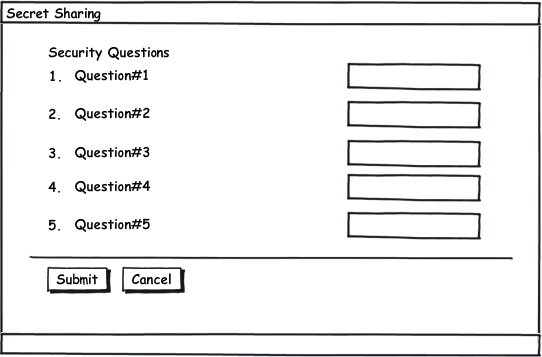
\includegraphics[scale=0.5]{Gambar/retrieve_password}}
	\caption{Perancangan Tampilan Mengembalikan \textit{Password}}\label{fig:retrieve_password}
\end{figure}

Pada bagian untuk mengembalikan \textit{password}, tampilannya cukup sederhana dan pengguna hanya cukup memasukkan setiap jawaban dari pertanyaan keamanan yang sudah dibuat sebelumnya di bagian penyimpanan password. Pada bagian ini, pengguna bebas untuk memilih mengisi setiap pertanyaan atau tidak menjawab pertanyaan keamanan. Setelah seluruh pertanyaan sudah dijawab, pengguna dapat menekan tombol "\textit{Submit}" yang kemudian akan menunjukkan \textit{password} pengguna.

Gambar \ref{fig:password} menunjukkan tampilan sesudah pengguna menekan tombol "\textit{Submit}" pada bagian di Gambar \ref{fig:retrieve_password}.

%diagram
\begin{figure}[H]
	\centerline{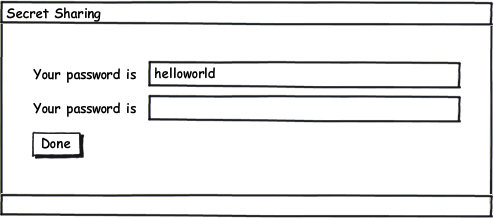
\includegraphics[scale=0.5]{Gambar/password}}
	\caption{Perancangan Tampilan Mengembalikan \textit{Password} (2)}\label{fig:password}
\end{figure}

Jika banyak pertanyaan keamanan yang dijawab benar oleh pengguna sesuai dengan minimal banyak pertanyaan keamanan yang dijawab benar maka pengguna bisa melihat \textit{password} yang sudah disimpan. Tapi, jika banyak pertanyaan keamanan yang dijawab benar oleh pengguna kurang dari minimal banyak pertanyaan keamanan yang harus dijawab benar maka pengguna tidak bisa melihat \textit{password} yang sudah disimpan.}{}
\ifdefstring{\vbabe}{1}{\chapter{Implementasi dan Pengujian}
\label{chap:Implementasi dan Pengujian}

Pada bab ini akan berisi mengenai implementasi perangkat lunak dan pengujian perangkat lunak yang dibangun.

\section{Implementasi Perangkat Lunak}

Pada bagian ini akan dibahas mengenai tampilan antarmuka perangkat lunak yang sudah dibangun.

\subsection{Tampilan Antarmuka Perangkat Lunak}

Tampilan antarmuka awal perangkat lunak dapat dilihat pada Gambar \ref{fig:tampilan1} dengan keterangan bagian-bagian sebagai berikut.

\begin{itemize}
	\item Bagian nomor 1 merupakan tombol untuk mengembalikan \textit{password}.
	\item Bagian nomor 2 merupakan tombol untuk menyimpan \textit{password}.
\end{itemize}

%diagram
\begin{figure}[H]
	\centerline{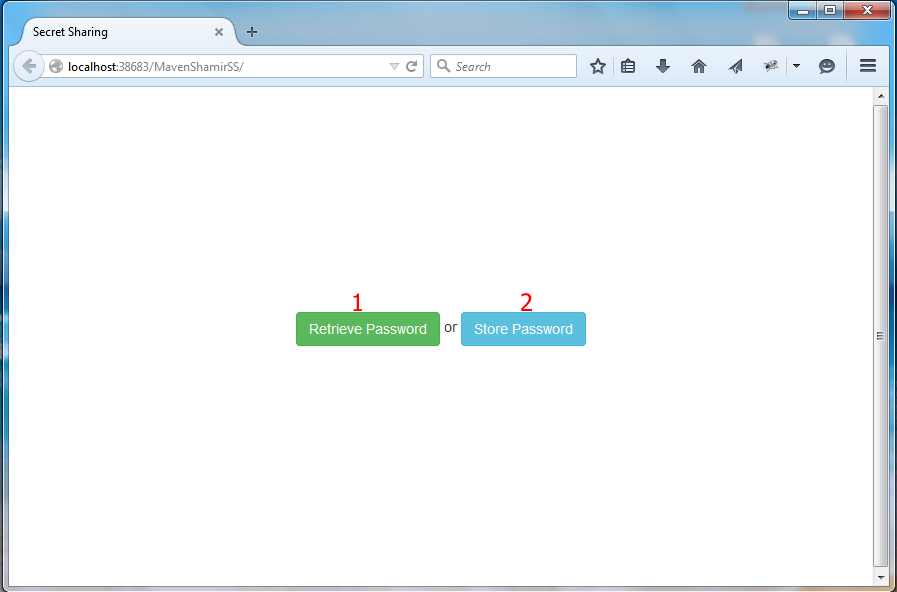
\includegraphics[scale=0.5]{Gambar/tampilan1}}
	\caption{Tampilan antarmuka awal}\label{fig:tampilan1}
\end{figure}

Setelah tombol \textit{"Store Password"} ditekan, tampilan antarmuka perangkat lunak akan terlihat seperti pada Gambar \ref{fig:tampilan2} dengan keterangan sebagai berikut.

\begin{itemize}
	\item Bagian nomor 3 merupakan tombol untuk menambah \textit{password}. Pengguna minimal harus menambahkan 1 \textit{password}, jika tidak maka akan muncul notifikasi seperti pada Gambar \ref{fig:tampilan2_2}.
	\item Bagian nomor 4 merupakan tombol untuk menambah pertanyaan keamanan.
	\item Bagian nomor 5 merupakan tombol untuk melanjutkan menyimpan \textit{password}.
	\item Bagian nomor 6 merupakan tombol untuk kembali ke tampilan antarmuka awal.
	\item Bagian nomor 7 merupakan teks masukan untuk pertanyaan keamanan yang hendak ditambahkan.
\end{itemize}

%diagram
\begin{figure}[H]
	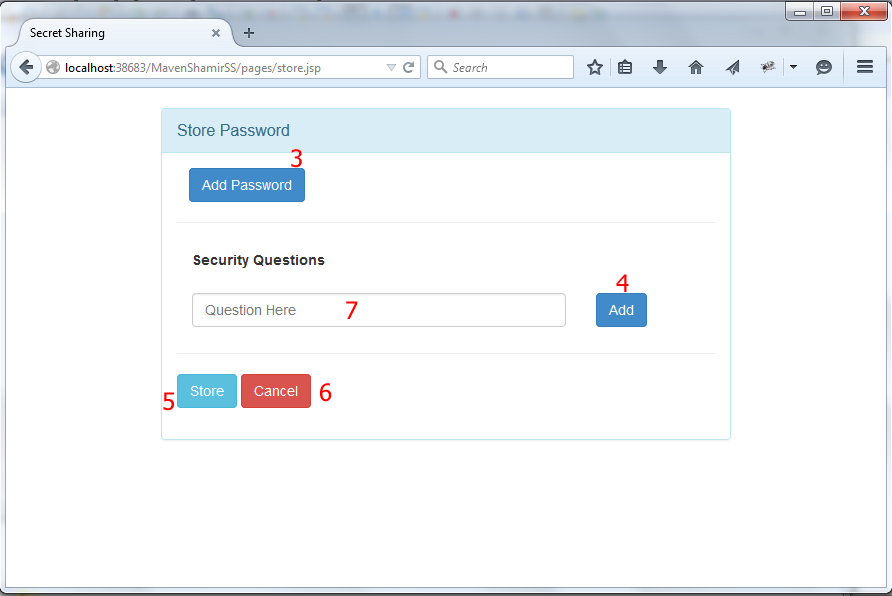
\includegraphics[scale=0.5]{Gambar/tampilan2}
	\centering
	\caption{Tampilan antarmuka untuk menyimpan \textit{password}}\label{fig:tampilan2}
\end{figure}

%diagram
\begin{figure}[H]
	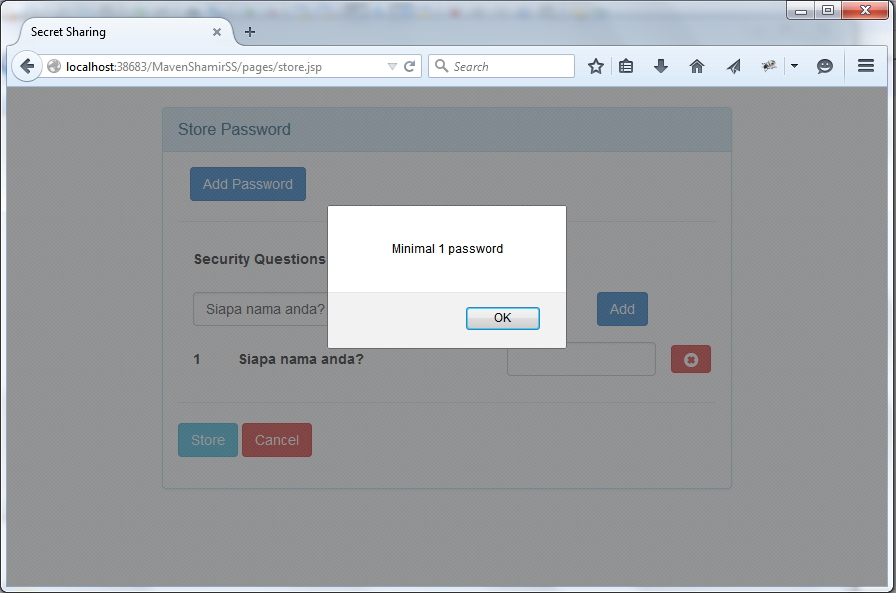
\includegraphics[scale=0.5]{Gambar/tampilan2_2}
	\centering
	\caption{Tampilan notifikasi pada antarmuka jika \textit{password} kurang}\label{fig:tampilan2_2}
\end{figure}

Setelah tombol \textit{"Add Password"} ditekan, maka tampilan antarmuka akan menambahkan masukkan teks untuk memasukkan \textit{password} yang hendak disimpan. Setelah tombol \textit{"Add"} ditekan, maka tampilan antarmuka akan menambahkan teks masukkan untuk jawaban dari pertanyaan keamanan yang sudah diisi di Bagian no 7. Tampilan yang ditunjukkan perangkat lunak dapat dilihat pada Gambar \ref{fig:tampilan2_1}.

%diagram
\begin{figure}[H]
	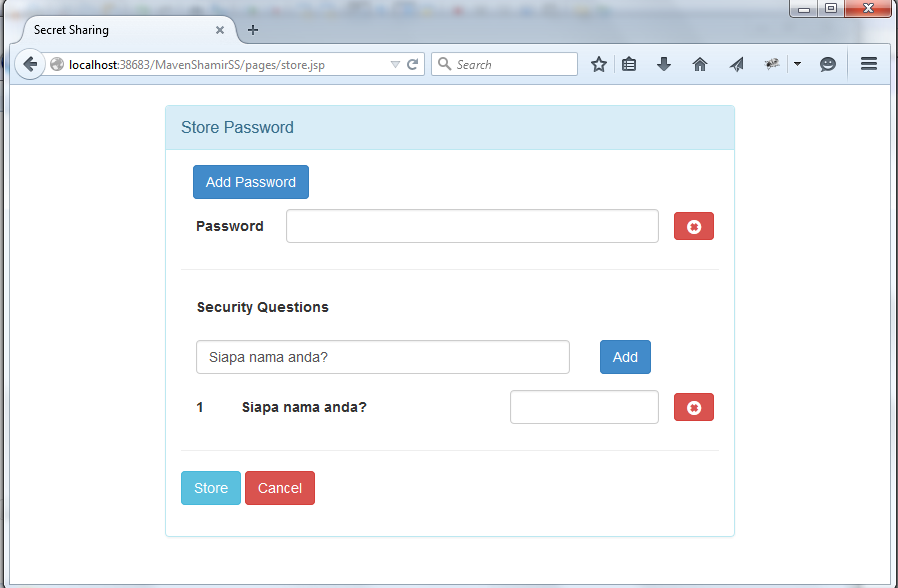
\includegraphics[scale=0.5]{Gambar/tampilan2_1}
	\centering
	\caption{Tampilan antarmuka menambah \textit{password}}\label{fig:tampilan2_1}
\end{figure}

Setelah tombol \textit{"Store"} ditekan, maka tampilan antarmuka perangkat lunak akan kembali ke tampilan antarmuka awal. \textit{Password} sudah berhasil disimpan. Kemudian, setelah tombol \textit{"Retrieve Password"} ditekan, maka tampilan perangkat lunak akan terlihat seperti pada Gambar \ref{fig:tampilan3} dengan keterangan sebagai berikut.

\begin{itemize}
	\item Bagian nomor 8 merupakan bagian dari pertanyaan keamanan yang harus dijawab oleh pengguna.
	\item Bagian nomor 9 merupakan bagian dari jawaban setiap pertanyaan keamanan yang harus dijawab.
	\item Bagian nomor 10 merupakan tombol untuk mengembalikan \textit{password}.
	\item Bagian nomor 11 merupakan tombol untuk kembali ke tampilan antarmuka awal.
\end{itemize}

%diagram
\begin{figure}[H]
	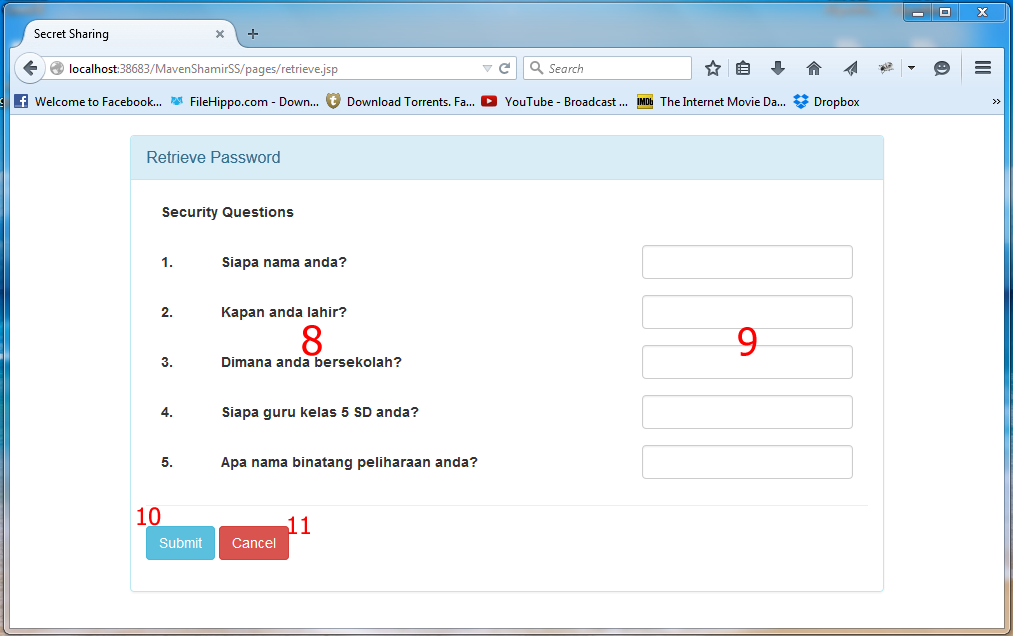
\includegraphics[scale=0.5]{Gambar/tampilan3}
	\centering
	\caption{Tampilan antarmuka untuk mengembalikan \textit{password}}\label{fig:tampilan3}
\end{figure}

Setelah tombol "Submit" pada Gambar \ref{fig:tampilan3} ditekan, perangkat lunak akan memroses setiap pertanyaan dan jawaban. Jika banyak jawaban benar dari pertanyaan keamanan yang dijawab oleh pengguna sesuai dengan minimal banyak pertanyaan keamanan yang dijawab benar yang sudah ditentukan sebelumnya, maka tampilan perangkat lunak akan terlihat seperti pada Gambar \ref{fig:tampilan4}.

%diagram
\begin{figure}[H]
	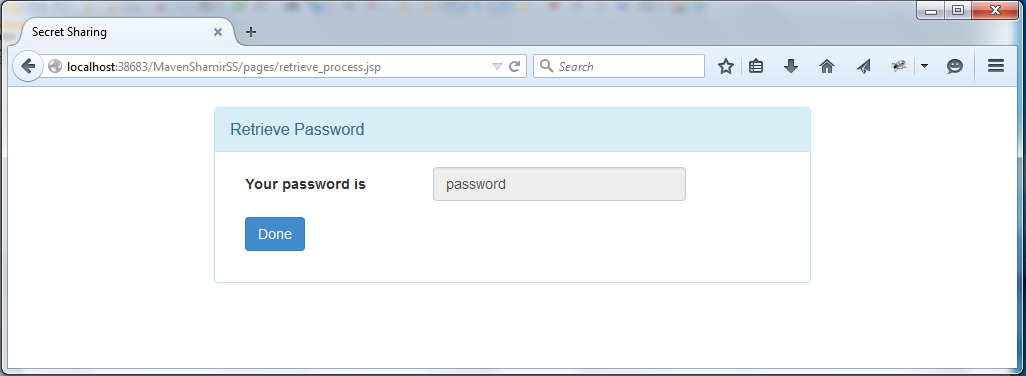
\includegraphics[scale=0.5]{Gambar/tampilan4}
	\centering
	\caption{Tampilan antarmuka untuk mengembalikan \textit{password} (2)}\label{fig:tampilan4}
\end{figure}

Sedangkan, jika pertanyaan keamanan yang dijawab benar kurang dari minimal pertanyaan keamanan yang harus dijawab benar, maka tampilan perangkat lunak akan menunjukkan notifikasi bahwa \textit{password} tidak bisa dikembalikan. Gambar \ref{fig:tampilan4_1} menunjukkan tampilan antarmuka perangkat lunak dengan notifikasi \textit{password} tidak bisa dikembalikan.

%diagram
\begin{figure}[H]
	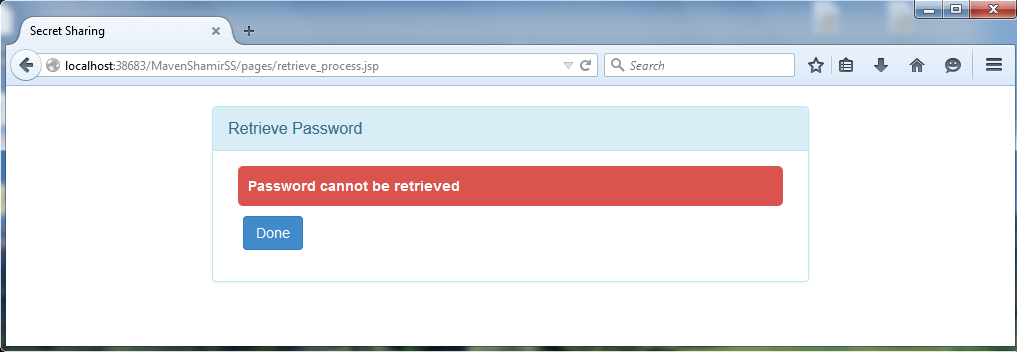
\includegraphics[scale=0.5]{Gambar/tampilan4_1}
	\centering
	\caption{Tampilan antarmuka untuk mengembalikan \textit{password} (3)}\label{fig:tampilan4_1}
\end{figure}

\section{Pengujian Perangkat Lunak}

Pada bagian ini akan berisi tentang metode pengujian, hasil pengujian, analisis pengujian, dan kesimpulan dari pengujian perangkat lunak yang sudah dibangun.

\subsection{Metode Pengujian}

Pengujian terhadap perangkat lunak yang sudah dibangun akan dibagi menjadi 2 bagian, yaitu pengujian fungsional dan pengujian suvei. Pada bagian ini akan dijelaskan masing-masing dari pengujian dan kasus yang akan digunakan dalam masing-masing pengujian yang dilakukan.

\subsubsection{Pengujian Fungsional}
	
Pengujian fungsional bertujuan untuk menguji apakah perangkat lunak dapat berfungsi sesuai dengan harapan. Dalam penelitian ini, perangkat lunak yang dibangun diharapkan dapat menyimpan \textit{password} dalam bentuk \textit{share-share} dan bisa mengembalikan banyak \textit{password} sekaligus dengan menjawab beberapa pertanyaan keamanan.

Kasus yang digunakan dalam pengujian fungsional terdiri dari 2 kasus. Kasus pertama adalah kasus dimana jika sebagian besar pertanyaan keamanan dapat dijawab dengan benar maka password akan bisa dikembalikan. Kasus kedua adalah kasus dimana jika pertanyaan keamanan yang dijawab benar tidak mencapai minimal pertanyaan keamanan yang dijawab benar sehingga password tidak bisa dikembalikan.

\subsubsection{Pengujian Survei}

Pengujian survei bertujuan untuk menguji kualitas dari pertanyaan keamanan yang dibuat saat proses menyimpan \textit{password}. Pengujian survei akan menguji pertanyaan keamanan dibuat berpengaruh pada mudah atau tidaknya \textit{password} bisa dikembalikan. Setiap pertanyaan ini akan dikelompokkan menjadi beberapa topik kasus yang sesuai dengan jenisnya.

Kasus yang digunakan dalam terdiri dari 4 kasus yang masing-masing terbagi atas topiknya masing-masing. Berikut penjelasan masing-masing topik kasus.

\begin{enumerate}[itemsep=0mm]
	\item Topik 1 \\
	Pertanyaan keamanan yang kemungkinan jawabannya hanya 2, yaitu Ya atau Tidak. Selain itu, dalam topik ini digunakan pertanyaan keamanan yang jawabannya bisa dicari di \textit{internet} atau media sosial.
	\item Topik 2 \\
	Pertanyaan keamanan yang sebagian besar jawabannya mengenai angka, seperti tanggal, bulan, tahun, dan sebagainya.
	\item Topik 3 \\
	Pertanyaan keamanan yang jawabannya mengenai hal-hal personal.
	\item Topik 4 \\
	Topik 4 akan berisi gabungan dari topik 1, topik 2, dan topik 3.
\end{enumerate}

Dalam pengujian survei ini, responden diberikan waktu tidak terbatas untuk mencoba menjawab pertanyaan keamanan yang sudah dibuat sampai \textit{password} dapat dikembalikan. Responden pun diberikan kebebasan untuk mengakses berbagai media sebagai bantuan untuk memperoleh jawaban dari setiap pertanyaan keamanan yang dibuat. Tetapi, responden tidak boleh menanyakan jawaban dari setiap pertanyaan keamanan yang dibuat kepada pembuat pertanyaan keamanan. Dalam pengujian survei ini juga, banyak percobaan untuk mengembalikan \textit{password} tidak dibatasi, responden boleh mencoba untuk mengembalikan password dengan menjawab pertanyaan keamanan yang dibuat sampai \textit{password} bisa dikembalikan atau responden tidak ingin mencoba lagi.

\subsection{Hasil Pengujian Fungsional}\label{subsec:hasil_pengujian_fungsional}

Sebelum dibahas hasil pengujian terhadap kasus-kasus yang sudah dijelaskan pada bagian metode pengujian fungsional, langkah pertama yang harus dilakukan adalah menyimpan \textit{password}. Untuk pengujian fungsional ini, $n$ yang dipilih adalah $n=5$ dan $k$ yang dipilih adalah $k=4$. Karena itu, ada 5 \textit{password} yang akan disimpan dan ada 5 pertanyaan keamanan yang dibuat untuk masing-masing \textit{password}. Langkah ini ditunjukkan pada Gambar \ref{fig:simpan_password}.

%diagram
\begin{figure}[H]
	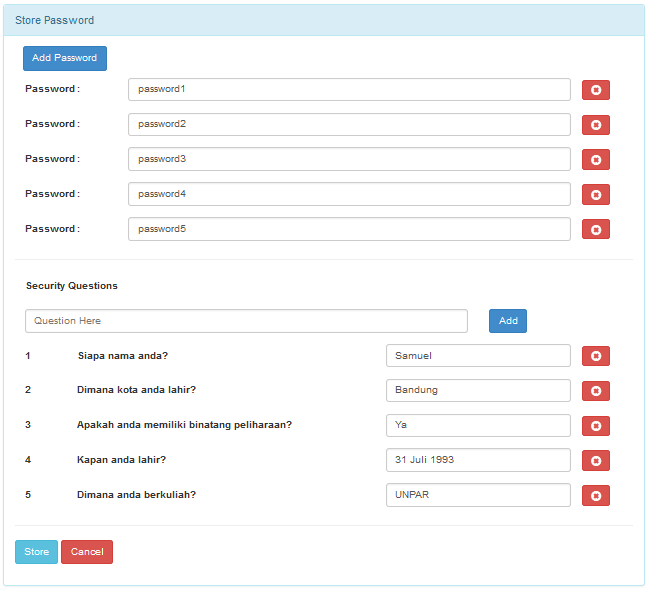
\includegraphics[scale=0.8]{Gambar/simpan_password}
	\centering
	\caption{Langkah menyimpan \textit{password}}\label{fig:simpan_password}
\end{figure}

Masukan password akan pada Gambar \ref{fig:simpan_password} ditunjukkan hanya sebagai bagian dari pengujian saja. Selanjutnya, setelah tombol "\textit{Store}" ditekan, maka password akan disimpan dan tampilan antarmuka perangkat lunak akan kembali ke tampilan antarmuka awal. Tampilan antarmuka awal ditunjukkan pada Gambar \ref{fig:tampilan1}.

Sesudah menyimpan password, langkah selanjutnya adalah melakukan pengujian terhadap kasus-kasus yang sudah dibahas pada bagian sebelumnya. Kasus pertama dari pengujian fungsional adalah kasus pertanyaan yang dijawab dengan benar sebanyak nilai $k$ atau lebih. Hasil yang diharapkan dari kasus pertama adalah password bisa dikembalikan karena banyak pertanyaan yang dijawab dengan benar sebanyak nilai $k$ atau lebih.

Langkah pertama yang perlu dilakukan dalam pengujian terhadap kasus-kasus adalah menjawab pertanyaan keamanan yang sudah disimpan. Untuk bisa menjawab pertanyaan keamanan yang sudah disimpan, tombol "\textit{Retrieve Password}" pada tampilan antarmuka awal harus ditekan. Setelah tombol tersebut ditekan, perangkat lunak akan menampilan tampilan pada Gambar \ref{fig:fungsional1}. Setiap pertanyaan pada Gambar \ref{fig:fungsional1} dijawab dengan mengisi masukan teks yang ada di samping masing-masing pertanyaan keamanan.

%diagram
\begin{figure}[H]
	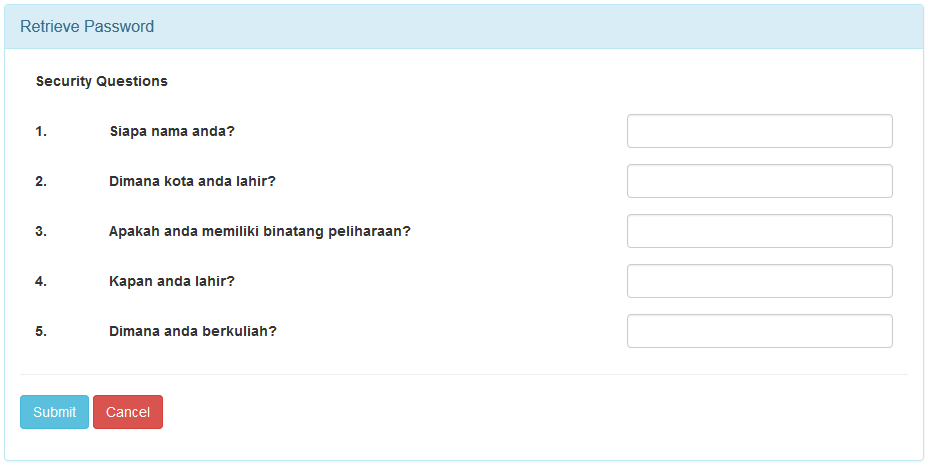
\includegraphics[scale=0.6]{Gambar/fungsional1}
	\centering
	\caption{Tampilan Menjawab Pertanyaan Keamanan}\label{fig:fungsional1}
\end{figure}

\subsubsection{Kasus 1}

Dalam kasus pertama, hasil yang diharapkan adalah password bisa dikembalikan. Maka dari itu, masukan teks ini akan diisi dengan jawaban yang benar dari masing-masing pertanyaan. Gambar \ref{fig:fungsional2} menunjukkan masukan teks yang sudah diisi dengan jawaban yang benar dari masing-masing pertanyaan.

%diagram
\begin{figure}[H]
	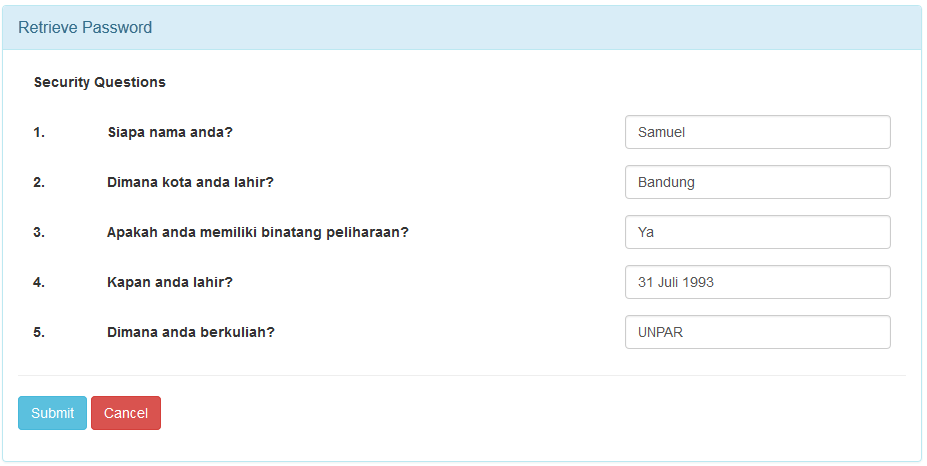
\includegraphics[scale=0.6]{Gambar/fungsional2}
	\centering
	\caption{Tampilan Menjawab Pertanyaan Keamanan Kasus Pertama}\label{fig:fungsional2}
\end{figure}

Setelah mengisi jawaban untuk masing-masing pertanyaan, langkah berikutnya adalah memroses jawaban dari masing-masing pertanyaan ini dengan metode skema threshold(k, n) yang sudah dibahas pada Bab \ref{sec:secretsharingshamir}. Untuk memroses hal ini, maka tombol "\textit{Submit}" pada Gambar \ref{fig:fungsional2} perlu ditekan.

Setelah tombol "Submit" pada Gambar \ref{fig:fungsional2} ditekan, perangkat lunak akan memroses setiap jawaban masing-masing pertanyaan. Dalam kasus pertama, seluruh pertanyaan bisa dijawab dengan benar, maka \textit{password} bisa dikembalikan. Gambar \ref{fig:fungsional3} menunjukkan bahwa \textit{password} bisa dikembalikan.

%diagram
\begin{figure}[H]
	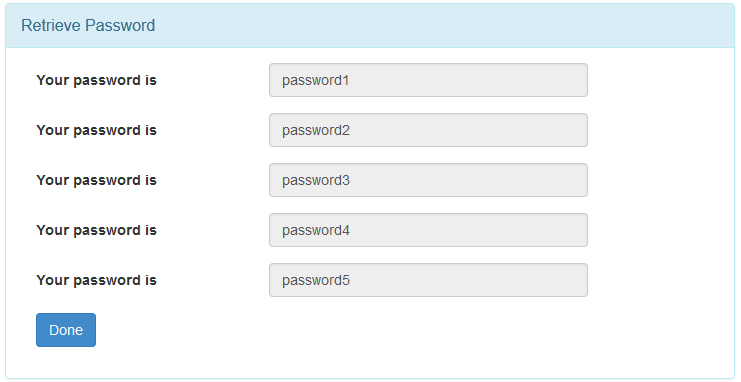
\includegraphics[scale=0.7]{Gambar/fungsional3}
	\centering
	\caption{Hasil Pengujian Fungsional Kasus Pertama}\label{fig:fungsional3}
\end{figure}

\subsubsection{Kasus 2}

Kasus selanjutnya adalah kasus kedua dimana \textit{password} tidak bisa dikembalikan. Dalam kasus ini, diasumsikan hanya 3 pertanyaan saja yang bisa dijawab dengan benar. Gambar \ref{fig:fungsional4} menunjukkan tampilan menjawab pertanyaan untuk kasus 2.

%diagram
\begin{figure}[H]
	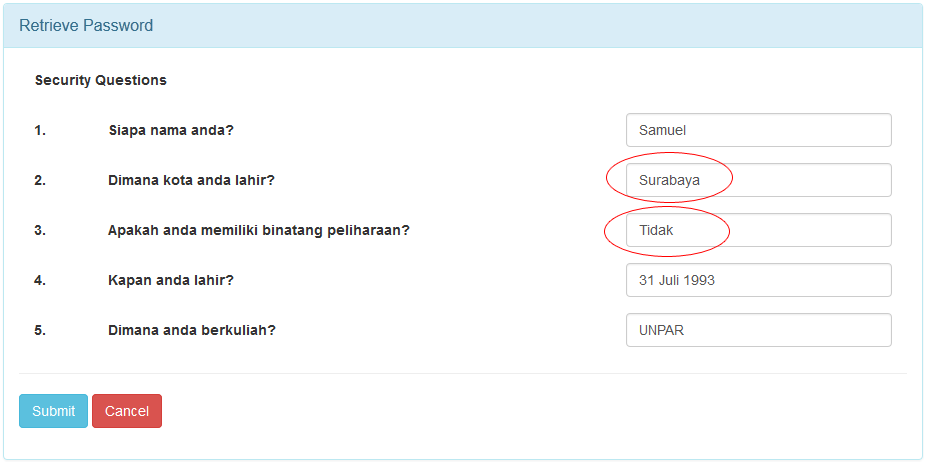
\includegraphics[scale=0.6]{Gambar/fungsional4}
	\centering
	\caption{Tampilan Menjawab Pertanyaan Keamanan Kasus Kedua}\label{fig:fungsional4}
\end{figure}

Pada Gambar \ref{fig:fungsional4} dapat dilihat bahwa hanya ada 3 pertanyaan yang dijawab dengan benar. Pertanyaan nomor 2 dan 3 diberi tanda untuk menunjukkan bahwa jawaban dari pertanyaan tersebut tidak tepat.

Langkah selanjutnya adalah memroses jawaban dari masing-masing pertanyaan dengan menekan tombol "\textit{Submit}". Setelah tombol "\textit{Submit}" ditekan, perangkat lunak akan menampilkan hasil pengujian kasus kedua. Dalam kasus kedua, karena $k$ yang dipilih $k=4$ dan hanya 3 pertanyaan yang dijawab dengan benar, maka \textit{password} tidak bisa dikembalikan. Gambar \ref{fig:fungsional5} menunjukkan langkah yang sudah dijelaskan.

%diagram
\begin{figure}[H]
	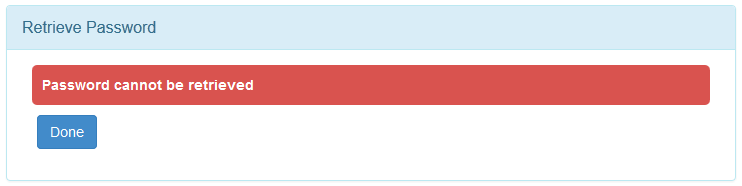
\includegraphics[scale=0.7]{Gambar/fungsional5}
	\centering
	\caption{Hasil Pengujian Fungsional Kasus Kedua}\label{fig:fungsional5}
\end{figure}

\subsection{Analisis Hasil Pengujian Fungsional}

Pada bagian ini akan dibahas analisis dari hasil pengujian fungsional yang sudah dilakukan. Seperti yang sudah dibahas, pengujian fungsional dibagi menjadi 2 kasus, yaitu kasus \textit{password} bisa dikembalikan dan kasus dimana \textit{password} tidak bisa dikembalikan.

Untuk kasus pertama, dapat dilihat bahwa jika pertanyaan keamanan yang dijawab benar lebih besar atau sama dengan nilai $k$ yang sudah ditentukan, maka semua password bisa dikembalikan. Dalam kasus pertama, seluruh pertanyaan dapat dijawab dengan benar, $pertanyaan benar = 5$. Kemudian untuk kasus pertama, nilai $k=4$ dan $pertanyaan benar > k$. Maka dari itu, \textit{password} bisa dikembalikan.

Untuk kasus kedua, dapat dilihat bahwa jika pertanyaan keamanan yang dijawab benar kurang dari $k$, maka password tidak bisa dikembalikan. Dalam kasus kedua, banyak pertanyaan yang dijawab benar hanya 3 pertanyaan, $pertanyaan benar=3$. Jadi, karena $k=4$ dan $pertanyaan benar < k$, \textit{password} tidak bisa dikembalikan.

Jadi, kesimpulan yang dapat diambil dari hasil pengujian kasus pertama dan kedua adalah perangkat lunak sudah bisa mengimplementasikan metode \textit{secret sharing} Shamir untuk mengembalikan $n$ password dengan menjawab $n$ pertanyaan.

\subsection{Analisis dan Hasil Pengujian Survei}\label{subsec:hasil_pengujian_survei}

Pada bagian ini akan ditunjukkan hasil pengujian survei. Seperti yang sudah dijelaskan, pengujian survei bertujuan untuk menilai kualitas dari pertanyaan keamanan dengan melihat tingkat kesulitan untuk menebak atau menjawab jawaban benar. Asumsi yang digunakan dalam pengujian ini adalah seluruh jawaban relevan dengan pertanyaan keamanan.

Pengujian survei ini terbagi atas 4 kasus. Responden melakukan survei dengan cara mencoba untuk menebak jawaban dari pertanyaan keamanan untuk mengembalikan password. Setiap orang bebas memilih cara untuk mendapatkan jawaban dari pertanyaan selain tidak bertanya kepada pembuat pertanyaan keamanan.

Kasus 1, 2, dan 3 memiliki 10 pertanyaan keamanan, $n=10$, dan minimal 4 pertanyaan keamanan dijawab benar, $k=4$. Sementara itu, untuk kasus 4 nilai $n$ dan $k$ ditambah. Dalam kasus 4, terdapat 15 pertanyaan keamanan, $n=15$, dan minimal 6 pertanyaan keamanan dijawab benar, $k=6$. Berikut tabel hasil survei untuk setiap kasus beserta dengan penjelasannya. Untuk kasus 1 dan 2 survei dilakukan terhadap 7 orang responden, sedangkan untuk kasus 3 dan 4 survei dilakukan terhadap 20 orang responden.

\subsubsection{Kasus 1}

Berikut daftar pertanyaan keamanan yang digunakan dalam kasus 1:

\begin{enumerate}[itemsep=0mm]
	\item Apa jenis kelamin anda? (Laki-laki/Perempuan)
	\item Apakah anda pernah ke luar negeri?
	\item Apakah anda mempunyai binatang peliharaan?
	\item Apakah anda bermain alat musik?
	\item Apakah anda pernah tidak naik kelas?
	\item Apakah anda pernah mengalami kecelakaan?
	\item Apakah anda menyukai kegiatan olahraga?
	\item Apa nama belakang anda?
	\item Siapa nama ibu anda?
	\item Siapa nama ayah anda?
\end{enumerate}

Kemudian, hasil dari survei kasus 1 ditunjukkan oleh Grafik \ref{fig:kasus1}.

%diagram
\begin{figure}[H]
	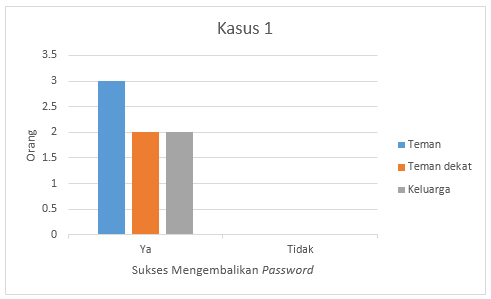
\includegraphics[scale=0.8]{Gambar/kasus1}
	\centering
	\caption{Pengujian survei kasus 1}\label{fig:kasus1}
\end{figure}

\subsubsection{Analisis Kasus 1}

Dilihat dari grafik \ref{fig:kasus1} untuk topik kasus 1, seluruh responden bisa berhasil mengembalikan \textit{password}. Hal ini karena mayoritas kemungkinan jawaban dari pertanyaan keamanan adalah kemungkinan biner dengan hanya 2 kemungkinan saja (Ya atau Tidak). Pertanyaan keamanan yang kemungkinan jawabannya hanya 2 kemungkinan saja bisa dengan mudah ditebak. Karena setiap jawaban bisa dengan mudah ditebak, maka seluruh responden bisa mengembalikan \textit{password} dengan mudah.

\subsubsection{Kasus 2}

Berikut daftar pertanyaan keamanan yang digunakan dalam kasus 2:

\begin{enumerate}[itemsep=0mm]
	\item Pada tahun berapa anda lahir?
	\item Pada tanggal berapa anda lahir?
	\item Pada bulan apa anda lahir?
	\item Berapa perbedaan umur anda dengan ayah anda?
	\item Berapa perbedaan umur anda dengan ibu anda?
	\item Berapa orang saudara anda?
	\item Berapa nomor rumah tempat anda tinggal?
	\item Dimana anda tinggal?
	\item Apa merek kendaraan yang anda pakai?
	\item Pada hari apa anda lahir?
\end{enumerate}

Kemudian, hasil dari survei kasus 2 ditunjukkan oleh Grafik \ref{fig:kasus2}.

%diagram
\begin{figure}[H]
	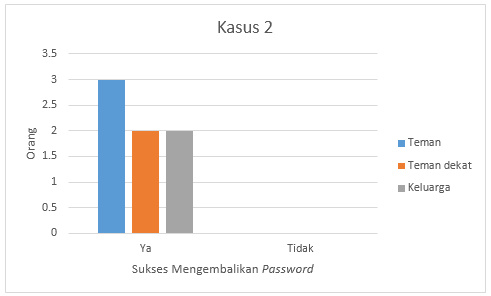
\includegraphics[scale=0.8]{Gambar/kasus2}
	\centering
	\caption{Pengujian survei kasus 2}\label{fig:kasus2}
\end{figure}

\subsubsection{Analisis Kasus 2}

Dilihat dari grafik \ref{fig:kasus2} untuk topik kasus 2, seluruh responden berhasil untuk mengembalikan password. Hal ini disebabkan karena kemungkinan jawaban dari pertanyaan keamanan hanya berupa angka saja, khususnya hanya tanggal ulang tahun, bulan lahir, atau tahun lahir.

Responden dapat menjawab tanggal lahir karena hanya memiliki 30-31 kemungkinan, sedangkan untuk bulan hanya ada 12 kemungkinan, dan juga beberapa pertanyaan lain yang menyangkut angka. Dapat dilihat juga, bahwa beberapa jawaban untuk pertanyaan keamanan merupakan informasi yang sering ditunjukkan dalam profil sosial media, karena dari itu jawaban yang tepat bisa dengan mudah didapatkan.

\subsubsection{Kasus 3}

Berikut daftar pertanyaan keamanan yang digunakan dalam kasus 3:

\begin{enumerate}[itemsep=0mm]
	\item Pada jam berapa anda lahir?(jj:mm)
	\item Apa nama sekolah dasar tempat anda bersekolah?
	\item Siapa nama belakang sepupu paling tua dari keluarga sisi ibu anda?
	\item Siapa nama belakang sepupu paling tua dari keluarga sisi ayah anda?
	\item Apa cita-cita anda dulu sewaktu kecil?
	\item Siapa nama anak paling tua dari nenek sisi ibu anda?
	\item Apa binatang peliharaan pertama anda?
	\item Apa alat musik yang anda mainkan pertama kali?
	\item Dimana kerabat terdekat anda tinggal/berasal?
	\item Siapa nama guru kelas 3 SD anda?
\end{enumerate}

Kemudian, hasil dari survei kasus 3 ditunjukkan oleh Grafik \ref{fig:kasus3}.

%diagram
\begin{figure}[H]
	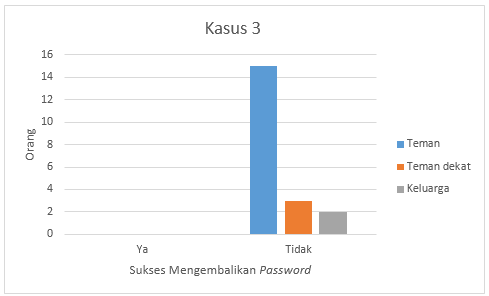
\includegraphics[scale=0.8]{Gambar/kasus3}
	\centering
	\caption{Pengujian survei kasus 3}\label{fig:kasus3}
\end{figure}

\subsubsection{Analisis Kasus 3}

Untuk topik kasus 3, tidak ada responden yang berhasil mengembalikan \textit{password}. Hal ini karena beberapa pertanyaan sifatnya sangat personal dan jawaban tidak bisa dengan mudah ditebak atau dicari di \textit{internet} atau media sosial. Pertanyaan yang sifatnya sangat personal akan mempersulit untuk mengembalikan \textit{password} kecuali bagi pembuat pertanyaan.

\subsubsection{Kasus 4}

Berikut daftar pertanyaan keamanan yang digunakan dalam kasus 4:

\begin{enumerate}[itemsep=0mm]
	\item Apakah anda mempunyai binatang peliharaan?
	\item Apakah anda bermain alat musik?
	\item Apakah anda pernah tidak naik kelas?
	\item Apa nama belakang anda?
	\item Siapa nama ibu anda?
	\item Pada hari apa anda lahir?
	\item Pada tanggal berapa anda lahir?
	\item Pada bulan apa anda lahir?
	\item Berapa perbedaan umur anda dengan ayah anda?
	\item Berapa nomor rumah tempat anda tinggal?
	\item Pada jam berapa anda lahir?(jj:mm)
	\item Apa cita-cita anda dulu sewaktu kecil?
	\item Siapa nama anak paling tua dari nenek sisi ibu anda?
	\item Apa binatang peliharaan pertama anda?
	\item Siapa nama guru kelas 3 SD anda?
\end{enumerate}

Kemudian, Grafik \ref{fig:kasus4} menunjukkan hasil survei kasus 4.

%diagram
\begin{figure}[H]
	\includegraphics[scale=0.8]{Gambar/kasus4}
	\centering
	\caption{Pengujian survei kasus 4}\label{fig:kasus4}
\end{figure}

\subsubsection{Analisis Kasus 4}

Dilihat dari grafik \ref{fig:kasus4} untuk topik kasus 4, tingkat keberhasilannya tetap tinggi walaupun topik kasus 4 ini merupakan gabungan dari topik kasus 1, 2, dan 3. Hal ini disebabkan karena mayoritas terdiri pertanyaan dari kasus 1 dan kasus 2.

Responden hanya cukup menjawab 6 pertanyaan benar dari 15 pertanyaan dalam kasus 4, maka responden pun cukup menjawab 3 pertanyaan dari kasus 1 dan 3 pertanyaan dari kasus 2 dengan benar, responden tidak perlu menjawab satupun pertanyaan dari kasus 3. Dapat disimpulkan, bahwa meningkatkan banyak pertanyaan keamanan tidak mempersulit untuk mengembalikan \textit{password}.

\subsection{Kesimpulan Pengujian}

Dari pengujian fungsional dan pengujian survei yang dilakukan maka bisa ditarik beberapa kesimpulan. Dari pengujian fungsional dapat ditarik kesimpulan bahwa pertanyaan keamanan yang dibuat sebaiknya memiliki sifat-sifat sebagai berikut.
\begin{enumerate}[itemsep=0mm]
	\item Stabil \\
	Pertanyaan keamanan tidak boleh berubah seiring berjalannya waktu.
	\item Mudah diingat \\
	Pertanyaan keamanan harus sifatnya personal sehingga mudah untuk diingat.
	\item Sederhana \\
	Pertanyaan keamanan harus sederhana tetapi sifatnya tetap personal.
\end{enumerate}

Sementara itu, dari hasil pengujian survei dapat ditarik kesimpulan bahwa pertanyaan keamanan yang dibuat sebaiknya juga memiliki sifa-sifat sebagai berikut.
\begin{enumerate}[itemsep=0mm]
	\item Aman \\
	Pertanyaan keamanan harus tidak mudah ditebak dan tidak mudah diselidiki jawabannya.
	\item Memiliki banyak kemungkinan jawaban \\
	Pertanyaan keamanan tidak boleh memiliki sedikit kemungkinan jawaban karena akan mudah ditebak.
\end{enumerate}

Namun, beberapa pertanyaan keamanan mungkin memiliki banyak kemungkinan jawaban dan aman sehingga tidak mudah ditebak tetapi tidak mudah diingat karena jawabannya terlalu rumit. Beberapa pertanyaan keamanan juga mungkin tidak sesuai dengan situasi atau keadaan dari pembuat pertanyaan. Sehingga, tidak ada pertanyaan keamanan yang memiliki seluruh sifat yang sudah dijelaskan di atas.}{}
\ifdefstring{\vbabf}{1}{\chapter{Kesimpulan dan Saran}
\label{chap:Kesimpulan dan Saran}

Bab ini berisi kesimpulan dan saran dari penelitian yang dilakukan. Kesimpulan akan menjawab rumusan masalah yang sudah dibuat pada Bab \ref{chap:Pendahuluan} dan saran akan berisi pengembangan lebih lanjut dari penelitian ini.

\section{Kesimpulan}

Dari hasil pengujian fungsional yang dilakukan, dapat dilihat bahwa pengguna cukup menjawab beberapa saja pertanyaan keamanan untuk mengembalikan banyak \textit{password} sehingga pengguna tidak perlu mengingat setiap jawaban dari pertanyaan keamanan. Dari hasil ini, dapat disimpulkan bahwa perangkat lunak yang mengimplementasikan \textit{secret sharing} Shamir berhasil dibangun. Dari pengujian fungsional yang sudah dilakukan juga, dapat ditarik kesimpulan bahwa pertanyaan keamanan yang dibuat sebaiknya juga memiliki sifa-sifat sebagai berikut.

\begin{enumerate}[itemsep=0mm]
	\item Stabil
	\item Mudah diingat
	\item Sederhana
\end{enumerate}

Dari hasil pengujian survei, dapat diambil hal penting yang berhubungan dengan pemilihan jenis pertanyaan keamanan yang dibuat. Jenis pertanyaan keamanan yang dibuat dapat dinilai dengan melihat 5 sifat berikut:

\begin{enumerate}[itemsep=0mm]
	\item Aman
	\item Memiliki banyak kemungkinan jawaban
\end{enumerate}

Dari hasil pengujian fungsional dan survei juga, dapat diketahui bahwa tidak ada pertanyaan keamanan yang memiliki seluruh sifat di atas, beberapa dari sifat di atas ada yang berlawanan sehingga tidak mungkin dapat dimiliki oleh sebuah pertanyaan keamanan sekaligus. Selain itu, jenis pertanyaan keamanan yang dibuat dapat mempengaruhi nilai entropi dari pertanyaan keamanan. Pertanyaan keamanan yang memiliki nilai entropi tinggi dapat dengan mudah ditebak atau diprediksi.

Jadi, dari hasil pengujian untuk penelitian yang dilakukan, dapat diambil kesimpulan bahwa metode \textit{secret sharing} Shamir dapat digunakan untuk mengembalikan $n$ password dengan $n$ pertanyaan keamanan, perangkat lunak pengingat \textit{password} yang mengimplementasikan metode \textit{secret sharing} Shamir berhasil dibangun, dan kualitas dari pertanyaan keamanan dapat dinilai dari 5 sifat yang sudah dipaparkan di atas.

\section{Saran}

Dari penelitian ini, terdapat beberapa saran untuk pengembangan perangkat lunak lebih lanjut, yaitu:
\begin{itemize}[itemsep=0mm]
	\item Algoritma enkripsi yang digunakan, yaitu \textit{data encryption standard} sebaiknya diganti dengan menggunakan algoritma enkripsi yang menggunakan panjang kunci lebih panjang dari 64-\textit{bit}.
	\item Metode \textit{secret sharing} Shamir diharapkan dapat diimplementasikan tidak hanya pada perangkat lunak perorangan seperti dalam penelitian ini, tetapi bisa diimplementasikan pada sebuah sistem besar yang memiliki subsistem dan masing-masing dari subsistem ini menyimpan banyak informasi penting.
	\item Banyak percobaan untuk mengembalikan \textit{password} harus dibatasi.
\end{itemize}}{}
\ifdefstring{\vbabg}{1}{\include{Bab/bab7}}{}
\ifdefstring{\vbabh}{1}{\include{Bab/bab8}}{}
\ifdefstring{\vbabi}{1}{\include{Bab/bab9}}{}

\bibliographystyle{ieeetr}
\bibliography{pustaka}

\appendix
\apptoc

\tampillmp{\vlmp}
\ifdefstring{\vlmpa}{1}{\chapter{The Source Code}
\label{app:A}

\singlespacing

\begin{lstlisting}[language=Java,basicstyle=\tiny,caption=DESEncryption.java]

package DES;

import java.util.ArrayList;

/**
 *
 * @author Samuel Christian
 */
public class DESEncryption {

    /**
     * ATTRIBUTES
     */

    //PC1 -> subkey permutation box
    private int[] PC1 = {
        57, 49, 41, 33, 25, 17, 9,
        1,  58, 50, 42, 34, 26, 18,
        10, 2,  59, 51, 43, 35, 27,
        19, 11, 3,  60, 52, 44, 36,
        63, 55, 47, 39, 31, 23, 15,
        7,  62, 54, 46, 38, 30, 22,
        14, 6,  61, 53, 45, 37, 29,
        21, 13, 5,  28, 20, 12, 4
    };

    //PC2 -> subkey permutatian final box
    private int[] PC2 = {
        14, 17, 11, 24, 1,  5,
        3,  28, 15, 6,  21, 10,
        23, 19, 12, 4,  26, 8,
        16, 7,  27, 20, 13, 2,
        41, 52, 31, 37, 47, 55,
        30, 40, 51, 45, 33, 48,
        44, 49, 39, 56, 34, 53,
        46, 42, 50, 36, 29, 32
    };

    //initial permutation
    private int[] IP = {
        58, 50, 42, 34, 26, 18, 10, 2,
        60, 52, 44, 36, 28, 20, 12, 4,
        62, 54, 46, 38, 30, 22, 14, 6,
        64, 56, 48, 40, 32, 24, 16, 8,
        57, 49, 41, 33, 25, 17, 9,  1,
        59, 51, 43, 35, 27, 19, 11, 3,
        61, 53, 45, 37, 29, 21, 13, 5,
        63, 55, 47, 39, 31, 23, 15, 7
    };

    //expansion P-box
    private int[] exp = {
        32, 1,  2,  3,  4,  5,
        4,  5,  6,  7,  8,  9,
        8,  9,  10, 11, 12, 13,
        12, 13, 14, 15, 16, 17,
        16, 17, 18, 19, 20, 21,
        20, 21, 22, 23, 24, 25,
        24, 25, 26, 27, 28, 29,
        28, 29, 30, 31, 32, 1
    };

    //s-boxes
    private int[][] s1 = {
        {14, 4, 14, 1, 2, 15, 11, 8, 3, 10, 6, 12, 5, 9, 0, 7},
        {0, 15, 7, 4, 14, 2, 13, 10, 3, 6, 12, 11, 9, 5, 3, 8},
        {4, 1, 14, 8, 13, 6, 2, 11, 15, 12, 9, 7, 3, 10, 5, 0},
        {15, 12, 8, 2, 4, 9, 1, 7, 5, 11, 3, 14, 10, 0, 6, 13}
    };
    private int[][] s2 = {
        {15, 1, 8, 14, 6, 11, 3, 4, 9, 7, 2, 13, 12, 0, 5, 10},
        {3, 13, 4, 7, 15, 2, 8, 14, 12, 0, 1, 10, 6, 9, 11, 5},
        {0, 14, 7, 11, 10, 4, 13, 1, 5, 8, 12, 6, 9, 3, 2, 15},
        {13, 8, 10, 1, 3, 15, 4, 2, 11, 6, 7, 12, 0, 5, 14, 9}
    };

    private int[][] s3 = {
        {10, 0, 9, 14, 6, 3, 15, 5, 1, 13, 12, 7, 11, 4, 2, 8},
        {13, 7, 0, 9, 3, 4, 6, 10, 2, 8, 5, 14, 12, 11, 15, 1},
        {13, 6, 4, 9, 8, 15, 3, 0, 11, 1, 2, 12, 5, 10, 14, 7},
        {1, 10, 13, 0, 6, 9, 8, 7, 4, 15, 14, 3, 11, 5, 2, 12}
    };

    private int[][] s4 = {
        {7, 13, 14, 3, 0, 6, 9, 10, 1, 2, 8, 5, 11, 12, 4, 15},
        {13, 8, 11, 5, 6, 15, 0, 3, 4, 7, 2, 12, 1, 10, 14, 9},
        {10, 6, 9, 0, 12, 11, 7, 13, 15, 1, 3, 14, 5, 2, 8, 4},
        {3, 15, 0, 6, 10, 1, 13, 8, 9, 4, 5, 11, 12, 7, 2, 14}
    };

    private int[][] s5 = {
        {2, 12, 4, 1, 7, 10, 11, 6, 8, 5, 3, 15, 13, 0, 14, 9},
        {14, 11, 2, 12, 4, 7, 13, 1, 5, 0, 15, 10, 3, 9, 8, 6},
        {4, 2, 1, 11, 10, 13, 7, 8, 15, 9, 12, 5, 6, 3, 0, 14},
        {11, 8, 12, 7, 1, 14, 2, 13, 6, 15, 0, 9, 10, 4, 5, 3}
    };

    private int[][] s6 = {
        {12, 1, 10, 15, 9, 2, 6, 8, 0, 13, 3, 4, 14, 7, 5, 11},
        {10, 15, 4, 2, 7, 12, 9, 5, 6, 1, 13, 14, 0, 11, 3, 8},
        {9, 14, 15, 5, 2, 8, 12, 3, 7, 0, 4, 10, 1, 13, 11, 6},
        {4, 3, 2, 12, 9, 5, 15, 10, 11, 14, 1, 7, 10, 0, 8, 13}
    };

    private int[][] s7 = {
        {4, 11, 2, 14, 15, 0, 8, 13, 3, 12, 9, 7, 5, 10, 6, 1},
        {13, 0, 11, 7, 4, 9, 1, 10, 14, 3, 5, 12, 2, 15, 8, 6},
        {1, 4, 11, 13, 12, 3, 7, 14, 10, 15, 6, 8, 0, 5, 9, 2},
        {6, 11, 13, 8, 1, 4, 10, 7, 9, 5, 0, 15, 14, 2, 3, 12}
    };

    private int[][] s8 = {
        {13, 2, 8, 4, 6, 15, 11, 1, 10, 9, 3, 14, 5, 0, 12, 7},
        {1, 15, 13, 8, 10, 3, 7, 4, 12, 5, 6, 11, 10, 14, 9, 2},
        {7, 11, 4, 1, 9, 12, 14, 2, 0, 6, 10, 13, 15, 3, 5, 8},
        {2, 1, 14, 7, 4, 10, 8, 13, 15, 12, 9, 0, 3, 5, 6, 11}
    };

    //straight permutation box after s-box substitution
    private int[] P = {
        16, 7,  20, 21,
        29, 12, 28, 17,
        1,  15, 23, 26,
        5,  18, 31, 10,
        2,  8,  24, 14,
        32, 27, 3,  9,
        19, 13, 30, 6,
        22, 11, 4,  25
    };

    //final permutation
    private int[] IP1 = {
        40, 8,  48, 16, 56, 24, 64, 32,
        39, 7,  47, 15, 55, 23, 63, 31,
        38, 6,  46, 14, 54, 22, 62, 30,
        37, 5,  45, 13, 53, 21, 61, 29,
        36, 4,  44, 12, 52, 20, 60, 28,
        35, 3,  43, 11, 51, 19, 59, 27,
        34, 2,  42, 10, 50, 18, 58, 26,
        33, 1,  41, 9,  49, 17, 57, 25
    };

    private String strMsg;
    private String strKey;
    private String msg;
    private String key;
    private String[] roundKey;
    private String cipher;
    private ArrayList<int[][]> sBox;
    private String[] msgBlock;

    public Encryption() {
        strMsg = "";
        strKey = "";
        msg = "";
        key = "";
        roundKey = new String[16];
        cipher = "";
        msgBlock = new String[1];

        sBox = new ArrayList<int[][]>();
        sBox.add(s1);
        sBox.add(s2);
        sBox.add(s3);
        sBox.add(s4);
        sBox.add(s5);
        sBox.add(s6);
        sBox.add(s7);
        sBox.add(s8);
    }

    public void reset() {
        strMsg = "";
        strKey = "";
        msg = "";
        key = "";
        roundKey = new String[16];
        cipher = "";
        msgBlock = new String[1];
    }

    public void encrypt() {
        createSubKey();
        String tempCipher = "";
        for(int block = 0; block < msgBlock.length; block++) {
            String init = initialPermutation(msgBlock[block]);
            String L0 = init.substring(0,init.length()/2);
            String R0 = init.substring(init.length()/2, init.length());

            //16 rounds
            String[] arr = {L0, R0};
            for(int i = 0; i < 16; i++) {
                arr = round(arr[0], arr[1], roundKey[i]);
            }

            tempCipher = arr[1] + arr[0];
            tempCipher = permute(tempCipher, IP1);
            cipher += tempCipher;
        }
    }

    public String getCipherText() {
        String cipherText = "";
        String[] temp = cipher.split("(?<=\\G.{4})");
        for(int i = 0; i < temp.length; i++) {
            cipherText += Integer.toHexString(Integer.parseInt(temp[i], 2));
        }
        return cipherText;
    }

    private String[] round(String left, String right, String rndKey) {
        String Ln = right;
        String Rn = xor(left, feistelCipher(right, rndKey));
        String[] arr = {Ln, Rn};
        return arr;
    }

    private String feistelCipher(String right, String rndKey) {
        String res = "";

        res = xor(rndKey, permute(right, exp));

        String[] B = res.split("(?<=\\G.{6})");
        String temp = "";
        for(int i = 0; i < sBox.size(); i++) {
            String index = B[i];
            int[][] sbox = sBox.get(i);
            int row = Integer.parseInt(index.charAt(0) + "" + index.charAt(index.length()-1) + "",2);
            int column = Integer.parseInt(index.substring(1, index.length()-1), 2);
            temp += String.format("%4s", Integer.toBinaryString(sbox[row][column])).replace(' ', '0');
        }

        res = permute(temp, P);

        return res;
    }

    private String initialPermutation(String msgblock) {
        String res = permute(msgblock, IP);
        return res;
    }

    private void createSubKey() {
        String K2 = permute(key, PC1);
        String left = K2.substring(0, K2.length()/2);
        String right = K2.substring(K2.length()/2, K2.length());
        for(int i = 0; i < 16 ; i++) {
            int shift = 2;
            int round = i + 1;
            if(round == 1 || round == 2 || round == 9 || round == 16) {
                shift = 1;
            }
            String leftN = leftShift(left, shift);
            String rightN = leftShift(right, shift);
            roundKey[i] = leftN+rightN;
            left = leftN;
            right = rightN;
        }

        for(int i = 0; i < roundKey.length; i++) {
            roundKey[i] = permute(roundKey[i], PC2);
        }
    }

    private String leftShift(String text, int bit) {
        String res = "";
        char[] ch = new char[text.length()];
        for(int i = 0; i < ch.length; i++) {
            int shift = (i-bit) < 0 ? text.length()+(i-bit) : (i-bit);
            ch[shift] = text.charAt(i);
        }
        res = new String(ch);
        return res;
    }

    public void initialize() {
        String tempMessage = "";
        for(int i = 0; i < strMsg.length(); i++) {
            tempMessage += String.format("%8s", Integer.toBinaryString(strMsg.charAt(i))).replace(' ', '0');
        }

        int padLength = (64 - (tempMessage.length() % 64)) / 8;
        String padding = "";
        for(int i = 0; i < padLength; i++) {
            padding += String.format("%8s", Integer.toBinaryString(32)).replace(' ', '0');
        }

        msg = tempMessage + padding;

        msgBlock = msg.split("(?<=\\G.{64})");

        for(int i = 0; i < strKey.length(); i++) {
            key += String.format("%8s", Integer.toBinaryString(strKey.charAt(i))).replace(' ', '0');
        }
    }
    public void setMessage(String m) {
        strMsg = m;
    }

    public void setKey(String k) {
        strKey = k;
    }

    private String permute(String text, int[] permutationBox) {
        String res = "";
        for(int i = 0; i < permutationBox.length; i++) {
            res += text.charAt(permutationBox[i]-1);
        }
        return res;
    }

    private String xor(String a, String b) {
        String res = "";
        for(int i = 0; i < a.length(); i++) {
            int temp1 = a.charAt(i)-48;
            int temp2 = b.charAt(i)-48;
            int xor = temp1 ^ temp2;
            res += xor;
        }
        return res;
    }
}

\end{lstlisting}

\begin{lstlisting}[language=Java,basicstyle=\tiny,caption=DESDecryption.java]

package DES;

import java.util.ArrayList;

/**
 *
 * @author Samuel Christian
 */
public class DESDecryption {

    /**
     * ATTRIBUTES
     */

    //PC1 -> subkey permutation box
    private int[] PC1 = {
        57, 49, 41, 33, 25, 17, 9,
        1,  58, 50, 42, 34, 26, 18,
        10, 2,  59, 51, 43, 35, 27,
        19, 11, 3,  60, 52, 44, 36,
        63, 55, 47, 39, 31, 23, 15,
        7,  62, 54, 46, 38, 30, 22,
        14, 6,  61, 53, 45, 37, 29,
        21, 13, 5,  28, 20, 12, 4
    };

    //PC2 -> subkey permutatian final box
    private int[] PC2 = {
        14, 17, 11, 24, 1,  5,
        3,  28, 15, 6,  21, 10,
        23, 19, 12, 4,  26, 8,
        16, 7,  27, 20, 13, 2,
        41, 52, 31, 37, 47, 55,
        30, 40, 51, 45, 33, 48,
        44, 49, 39, 56, 34, 53,
        46, 42, 50, 36, 29, 32
    };

    //initial permutation
    private int[] IP = {
        58, 50, 42, 34, 26, 18, 10, 2,
        60, 52, 44, 36, 28, 20, 12, 4,
        62, 54, 46, 38, 30, 22, 14, 6,
        64, 56, 48, 40, 32, 24, 16, 8,
        57, 49, 41, 33, 25, 17, 9,  1,
        59, 51, 43, 35, 27, 19, 11, 3,
        61, 53, 45, 37, 29, 21, 13, 5,
        63, 55, 47, 39, 31, 23, 15, 7
    };

    //expansion P-box
    private int[] exp = {
        32, 1,  2,  3,  4,  5,
        4,  5,  6,  7,  8,  9,
        8,  9,  10, 11, 12, 13,
        12, 13, 14, 15, 16, 17,
        16, 17, 18, 19, 20, 21,
        20, 21, 22, 23, 24, 25,
        24, 25, 26, 27, 28, 29,
        28, 29, 30, 31, 32, 1
    };

    //s-boxes
    private int[][] s1 = {
        {14, 4, 14, 1, 2, 15, 11, 8, 3, 10, 6, 12, 5, 9, 0, 7},
        {0, 15, 7, 4, 14, 2, 13, 10, 3, 6, 12, 11, 9, 5, 3, 8},
        {4, 1, 14, 8, 13, 6, 2, 11, 15, 12, 9, 7, 3, 10, 5, 0},
        {15, 12, 8, 2, 4, 9, 1, 7, 5, 11, 3, 14, 10, 0, 6, 13}
    };
    private int[][] s2 = {
        {15, 1, 8, 14, 6, 11, 3, 4, 9, 7, 2, 13, 12, 0, 5, 10},
        {3, 13, 4, 7, 15, 2, 8, 14, 12, 0, 1, 10, 6, 9, 11, 5},
        {0, 14, 7, 11, 10, 4, 13, 1, 5, 8, 12, 6, 9, 3, 2, 15},
        {13, 8, 10, 1, 3, 15, 4, 2, 11, 6, 7, 12, 0, 5, 14, 9}
    };

    private int[][] s3 = {
        {10, 0, 9, 14, 6, 3, 15, 5, 1, 13, 12, 7, 11, 4, 2, 8},
        {13, 7, 0, 9, 3, 4, 6, 10, 2, 8, 5, 14, 12, 11, 15, 1},
        {13, 6, 4, 9, 8, 15, 3, 0, 11, 1, 2, 12, 5, 10, 14, 7},
        {1, 10, 13, 0, 6, 9, 8, 7, 4, 15, 14, 3, 11, 5, 2, 12}
    };

    private int[][] s4 = {
        {7, 13, 14, 3, 0, 6, 9, 10, 1, 2, 8, 5, 11, 12, 4, 15},
        {13, 8, 11, 5, 6, 15, 0, 3, 4, 7, 2, 12, 1, 10, 14, 9},
        {10, 6, 9, 0, 12, 11, 7, 13, 15, 1, 3, 14, 5, 2, 8, 4},
        {3, 15, 0, 6, 10, 1, 13, 8, 9, 4, 5, 11, 12, 7, 2, 14}
    };

    private int[][] s5 = {
        {2, 12, 4, 1, 7, 10, 11, 6, 8, 5, 3, 15, 13, 0, 14, 9},
        {14, 11, 2, 12, 4, 7, 13, 1, 5, 0, 15, 10, 3, 9, 8, 6},
        {4, 2, 1, 11, 10, 13, 7, 8, 15, 9, 12, 5, 6, 3, 0, 14},
        {11, 8, 12, 7, 1, 14, 2, 13, 6, 15, 0, 9, 10, 4, 5, 3}
    };

    private int[][] s6 = {
        {12, 1, 10, 15, 9, 2, 6, 8, 0, 13, 3, 4, 14, 7, 5, 11},
        {10, 15, 4, 2, 7, 12, 9, 5, 6, 1, 13, 14, 0, 11, 3, 8},
        {9, 14, 15, 5, 2, 8, 12, 3, 7, 0, 4, 10, 1, 13, 11, 6},
        {4, 3, 2, 12, 9, 5, 15, 10, 11, 14, 1, 7, 10, 0, 8, 13}
    };

    private int[][] s7 = {
        {4, 11, 2, 14, 15, 0, 8, 13, 3, 12, 9, 7, 5, 10, 6, 1},
        {13, 0, 11, 7, 4, 9, 1, 10, 14, 3, 5, 12, 2, 15, 8, 6},
        {1, 4, 11, 13, 12, 3, 7, 14, 10, 15, 6, 8, 0, 5, 9, 2},
        {6, 11, 13, 8, 1, 4, 10, 7, 9, 5, 0, 15, 14, 2, 3, 12}
    };

    private int[][] s8 = {
        {13, 2, 8, 4, 6, 15, 11, 1, 10, 9, 3, 14, 5, 0, 12, 7},
        {1, 15, 13, 8, 10, 3, 7, 4, 12, 5, 6, 11, 10, 14, 9, 2},
        {7, 11, 4, 1, 9, 12, 14, 2, 0, 6, 10, 13, 15, 3, 5, 8},
        {2, 1, 14, 7, 4, 10, 8, 13, 15, 12, 9, 0, 3, 5, 6, 11}
    };

    //straight permutation box after s-box substitution
    private int[] P = {
        16, 7,  20, 21,
        29, 12, 28, 17,
        1,  15, 23, 26,
        5,  18, 31, 10,
        2,  8,  24, 14,
        32, 27, 3,  9,
        19, 13, 30, 6,
        22, 11, 4,  25
    };

    //final permutation
    private int[] IP1 = {
        40, 8,  48, 16, 56, 24, 64, 32,
        39, 7,  47, 15, 55, 23, 63, 31,
        38, 6,  46, 14, 54, 22, 62, 30,
        37, 5,  45, 13, 53, 21, 61, 29,
        36, 4,  44, 12, 52, 20, 60, 28,
        35, 3,  43, 11, 51, 19, 59, 27,
        34, 2,  42, 10, 50, 18, 58, 26,
        33, 1,  41, 9,  49, 17, 57, 25
    };

    private String key;
    private String[] roundKey;
    private String cipher;
    private ArrayList<int[][]> sBox;

    public DESDecryption() {
        key = "";
        roundKey = new String[16];
        cipher = "";

        sBox = new ArrayList<int[][]>();
        sBox.add(s1);
        sBox.add(s2);
        sBox.add(s3);
        sBox.add(s4);
        sBox.add(s5);
        sBox.add(s6);
        sBox.add(s7);
        sBox.add(s8);
    }

    public void reset() {
        key = "";
        roundKey = new String[16];
        cipher = "";
    }

    public void setCipher(String c) {
        String bin = "";
        for(int i = 0; i < c.length(); i++) {
            int hex = Integer.parseInt(c.charAt(i)+"", 16);
            String temp = String.format("%4s", Integer.toBinaryString(hex)).replace(' ', '0');
            bin += temp;
        }
        cipher = bin;
    }

    public void setKey(String k) {
        for(int i = 0; i < k.length(); i++) {
            key += String.format("%8s", Integer.toBinaryString(k.charAt(i))).replace(' ', '0');
        }
    }

    public String decrypt() {
        createSubKey();
        String plainText = "";

        String[] cipherBlock = cipher.split("(?<=\\G.{64})");

        for(int block = 0; block < cipherBlock.length; block++) {
            String init = initialPermutation(cipherBlock[block]);
            String L0 = init.substring(0,init.length()/2);
            String R0 = init.substring(init.length()/2, init.length());

            //16 rounds inverse
            String[] arr = {L0, R0};
            for(int i = 15; i >= 0; i--) {
                arr = round(arr[0], arr[1], roundKey[i]);
            }

            String tempPlainText = arr[1] + arr[0];
            tempPlainText = permute(tempPlainText, IP1);
            plainText += tempPlainText;
        }

        return plainText;
    }

    private String[] round(String left, String right, String rndKey) {
        String Ln = right;
        String Rn = xor(left, feistelCipher(right, rndKey));
        String[] arr = {Ln, Rn};
        return arr;
    }

    private String feistelCipher(String right, String rndKey) {
        String res = "";

        res = xor(rndKey, permute(right, exp));

        String[] B = res.split("(?<=\\G.{6})");
        String temp = "";
        for(int i = 0; i < sBox.size(); i++) {
            String index = B[i];
            int[][] sbox = sBox.get(i);
            int row = Integer.parseInt(index.charAt(0) + "" + index.charAt(index.length()-1) + "",2);
            int column = Integer.parseInt(index.substring(1, index.length()-1), 2);
            temp += String.format("%4s", Integer.toBinaryString(sbox[row][column])).replace(' ', '0');
        }

        res = permute(temp, P);

        return res;
    }

    private String initialPermutation(String msgblock) {
        String res = permute(msgblock, IP);
        return res;
    }

    private void createSubKey() {
        String K2 = permute(key, PC1);
        String left = K2.substring(0, K2.length()/2);
        String right = K2.substring(K2.length()/2, K2.length());
        for(int i = 0; i < 16 ; i++) {
            int shift = 2;
            int round = i + 1;
            if(round == 1 || round == 2 || round == 9 || round == 16) {
                shift = 1;
            }
            String leftN = leftShift(left, shift);
            String rightN = leftShift(right, shift);
            roundKey[i] = leftN+rightN;
            left = leftN;
            right = rightN;
        }

        for(int i = 0; i < roundKey.length; i++) {
            roundKey[i] = permute(roundKey[i], PC2);
        }
    }

    private String leftShift(String text, int bit) {
        String res = "";
        char[] ch = new char[text.length()];
        for(int i = 0; i < ch.length; i++) {
            int shift = (i-bit) < 0 ? text.length()+(i-bit) : (i-bit);
            ch[shift] = text.charAt(i);
        }
        res = new String(ch);
        return res;
    }

    private String permute(String text, int[] permutationBox) {
        String res = "";
        for(int i = 0; i < permutationBox.length; i++) {
            res += text.charAt(permutationBox[i]-1);
        }
        return res;
    }

    private String xor(String a, String b) {
        String res = "";
        for(int i = 0; i < a.length(); i++) {
            int temp1 = a.charAt(i)-48;
            int temp2 = b.charAt(i)-48;
            int xor = temp1 ^ temp2;
            res += xor;
        }
        return res;
    }

    public String binToStr(String bin) {
        String text = "";
        String[] temp = bin.split("(?<=\\G.{8})");
        for(int i = 0; i < temp.length; i++) {
            text += (char)Integer.parseInt(temp[i], 2);
        }
        return text;
    }
}

\end{lstlisting}

\begin{lstlisting}[language=Java,basicstyle=\tiny,caption=DataReader.java]

package ReaderWriter;

import java.io.BufferedReader;
import java.io.FileReader;
import java.io.IOException;
import java.util.ArrayList;

/**
 *
 * @author Samuel Christian
 */
public class DataReader {

    /**
     * ATTRIBUTES
     */
    private String filename;
    private ArrayList<String> content;

    public DataReader(String file) {
        filename = file;
        content = new ArrayList<String>();
    }

    public String[] get() {
        String[] str = new String[content.size()];
        for(int i = 0; i < str.length; i++) {
            str[i] = content.get(i);
        }
        return str;
    }

    public void read() {
        BufferedReader br = null;
        try {
            String sCurrentLine;
            br = new BufferedReader(new FileReader(filename));
            while ((sCurrentLine = br.readLine()) != null) {
                content.add(sCurrentLine);
            }
        } catch (IOException e) {
        } finally {
            try {
                if (br != null) {
                    br.close();
                }
            } catch (IOException ex) {
            }
        }
    }
}

\end{lstlisting}

\begin{lstlisting}[language=Java,basicstyle=\tiny,caption=DataWriter.java]

package ReaderWriter;

import java.io.BufferedWriter;
import java.io.File;
import java.io.FileWriter;
import java.io.IOException;

/**
 *
 * @author Samuel Christian
 */
public class DataWriter {

    /**
     * ATTRIBUTES
     */
    private String filename;
    private String content;

    public DataWriter(String name) {
        filename = name;
    }

    public void write(String text) throws IOException {
        content = text;
        try {
            File file = new File(filename);
            
            file.createNewFile();

            FileWriter fw = new FileWriter(file.getAbsoluteFile(), false);
            BufferedWriter bw = new BufferedWriter(fw);
            bw.write(content);
            bw.close();

            System.out.println("Done");

        } catch (IOException e) {
        }
    }
}

\end{lstlisting}

\begin{lstlisting}[language=Java,basicstyle=\tiny,caption=Sha512.java]

package SHA512;

import java.math.BigInteger;

/**
 *
 * @author Samuel Christian
 */
public class Sha512 {

    /**
     * ATTRIBUTES
     */

    /*Initial values*/
    private static final long[] INITIALS = {0x6a09e667f3bcc908L,
                                            0xbb67ae8584caa73bL,
                                            0x3c6ef372fe94f82bL,
                                            0xa54ff53a5f1d36f1L,
                                            0x510e527fade682d1L,
                                            0x9b05688c2b3e6c1fL,
                                            0x1f83d9abfb41bd6bL,
                                            0x5be0cd19137e2179L};

    /*Constants for 80 rounds in sha512*/
    private static final long[] CONSTANTS  =
                                  {0x428a2f98d728ae22L, 0x7137449123ef65cdL, 0xb5c0fbcfec4d3b2fL, 0xe9b5dba58189dbbcL,
                                   0x3956c25bf348b538L, 0x59f111f1b605d019L, 0x923f82a4af194f9bL, 0xab1c5ed5da6d8118L,
                                   0xd807aa98a3030242L, 0x12835b0145706fbeL, 0x243185be4ee4b28cL, 0x550c7dc3d5ffb4e2L,
                                   0x72be5d74f27b896fL, 0x80deb1fe3b1696b1L, 0x9bdc06a725c71235L, 0xc19bf174cf692694L,
                                   0xe49b69c19ef14ad2L, 0xefbe4786384f25e3L, 0x0fc19dc68b8cd5b5L, 0x240ca1cc77ac9c65L,
                                   0x2de92c6f592b0275L, 0x4a7484aa6ea6e483L, 0x5cb0a9dcbd41fbd4L, 0x76f988da831153b5L,
                                   0x983e5152ee66dfabL, 0xa831c66d2db43210L, 0xb00327c898fb213fL, 0xbf597fc7beef0ee4L,
                                   0xc6e00bf33da88fc2L, 0xd5a79147930aa725L, 0x06ca6351e003826fL, 0x142929670a0e6e70L,
                                   0x27b70a8546d22ffcL, 0x2e1b21385c26c926L, 0x4d2c6dfc5ac42aedL, 0x53380d139d95b3dfL,
                                   0x650a73548baf63deL, 0x766a0abb3c77b2a8L, 0x81c2c92e47edaee6L, 0x92722c851482353bL,
                                   0xa2bfe8a14cf10364L, 0xa81a664bbc423001L, 0xc24b8b70d0f89791L, 0xc76c51a30654be30L,
                                   0xd192e819d6ef5218L, 0xd69906245565a910L, 0xf40e35855771202aL, 0x106aa07032bbd1b8L,
                                   0x19a4c116b8d2d0c8L, 0x1e376c085141ab53L, 0x2748774cdf8eeb99L, 0x34b0bcb5e19b48a8L,
                                   0x391c0cb3c5c95a63L, 0x4ed8aa4ae3418acbL, 0x5b9cca4f7763e373L, 0x682e6ff3d6b2b8a3L,
                                   0x748f82ee5defb2fcL, 0x78a5636f43172f60L, 0x84c87814a1f0ab72L, 0x8cc702081a6439ecL,
                                   0x90befffa23631e28L, 0xa4506cebde82bde9L, 0xbef9a3f7b2c67915L, 0xc67178f2e372532bL,
                                   0xca273eceea26619cL, 0xd186b8c721c0c207L, 0xeada7dd6cde0eb1eL, 0xf57d4f7fee6ed178L,
                                   0x06f067aa72176fbaL, 0x0a637dc5a2c898a6L, 0x113f9804bef90daeL, 0x1b710b35131c471bL,
                                   0x28db77f523047d84L, 0x32caab7b40c72493L, 0x3c9ebe0a15c9bebcL, 0x431d67c49c100d4cL,
                                   0x4cc5d4becb3e42b6L, 0x597f299cfc657e2aL, 0x5fcb6fab3ad6faecL, 0x6c44198c4a475817L};

    private String originalMessage;
    private String lengthMessage;
    private String paddingMessage;
    private String message;
    private String[] messageBlock;
    private String digest;

    public Sha512() {
        message = "";
        lengthMessage = "";
        paddingMessage = "";
        originalMessage = "";
        digest = "";
    }

    public void setMessage(String m) {
        reset();
        message = m;
    }

    public void reset() {
        message = "";
        lengthMessage = "";
        paddingMessage = "";
        originalMessage = "";
        digest = "";
    }

    public String getDigest() {
        String text = "";
        for(int i = 0; i < digest.length(); i+=4) {
            String bits = digest.substring(i, i+4);
            text += Long.toHexString(longValue(bits));
        }
        return text;
    }

    public void createDigest() {
        initialize(message);
        String[] finalDigest = new String[INITIALS.length];
        for(int countBlock = 0; countBlock < messageBlock.length; countBlock++) {
            String block = messageBlock[countBlock];
            String[] words = wordsExpansion(block);
            String[] first = finalDigest;
            
            //initialize first digest
            if(countBlock == 0) {
                for(int i = 0; i < finalDigest.length; i++) {
                    finalDigest[i] = pad(Long.toBinaryString(INITIALS[i]));
                }
            }

            //80 rounds
            for(int i = 0; i < words.length; i++) {
                finalDigest = round(finalDigest, longValue(words[i]), i);
            }

            //final adding
            for(int i = 0; i < finalDigest.length; i++) {
                finalDigest[i] = pad(Long.toBinaryString(longValue(finalDigest[i]) + longValue(first[i])));
            }
        }
        for(int i = 0; i < finalDigest.length; i++) {
            digest += finalDigest[i] + "";
        }
    }

    private String[] wordsExpansion(String block) {
        String[] words = new String[80];
        for(int i = 0; i < 16; i++) {
            int start = i * 64;
            int end = start + 64;
            words[i] = block.substring(start, end);
        }
        for(int i = 16; i < words.length; i++) {
            //i-16
            long w1 = longValue(words[i-16]);

            //RotShift_1-8-7(i-15)
            long w2 = rotShift(longValue(words[i-15]), 1, 8, 7);

            //i-7
            long w3 = longValue(words[i-7]);

            //RotShift_19-61-6(i-2)
            long w4 = rotShift(longValue(words[i-2]), 19, 61, 6);

            long temp = w1 ^ w2 ^ w3 ^ w4;
            words[i] = pad(Long.toBinaryString(temp));
        }

        return words;
    }

    //preDigest: previous digest or initial digest
    //prevDigest[0] -> A    prevDigest[1] -> B    prevDigest[2] -> C    prevDigest[3] -> D
    //prevDigest[4] -> E    prevDigest[5] -> F    prevDigest[6] -> G    prevDigest[7] -> H
    private String[] round(String[] prevDigest, long word, int numOfRounds) {
        String[] result = new String[8];
        result[1] = pad(prevDigest[0]); //A -> B
        result[2] = pad(prevDigest[1]); //B -> C
        result[3] = pad(prevDigest[2]); //C -> D
        result[5] = pad(prevDigest[4]); //E -> F
        result[6] = pad(prevDigest[5]); //F -> G
        result[7] = pad(prevDigest[6]); //G -> H

        //compute Y -> E (prevDigest[4])
        //conditional(E,F,G)
        long cond = conditional(longValue(prevDigest[4]),longValue(prevDigest[5]),longValue(prevDigest[6]));
        //rotate(E)
        long rot_E = rotate(longValue(prevDigest[4]));
        //addition modulo 2^64
        //temp1 = H + cond(E,F,G) + rotate(E) + w_i + K_i
        long temp1 = longValue(prevDigest[7]) + cond + rot_E + word + CONSTANTS[numOfRounds];
        //Y = temp1 + D
        long Y = temp1 + longValue(prevDigest[3]);
        //Y -> E
        result[4] = pad(Long.toBinaryString(Y));

        //compute X -> A (prevDigest[0])
        //majority(A,B,C)
        long maj = majority(longValue(prevDigest[0]),longValue(prevDigest[1]),longValue(prevDigest[2]));
        //rotate(A)
        long rot_A = rotate(longValue(prevDigest[0]));
        //temp2 = majority(A,B,C) + rotate(A)
        long temp2 = maj + rot_A;
        //X = temp1 + temp2
        long X = temp1 + temp2;
        //X -> A
        result[0] = pad(Long.toBinaryString(X));

        return result;
    }

    /*WORD EXPANSION FUNCTIONS*/
    //RotShift_l-m-n(x) = RotR_l(x) XOR RotR_m(x) XOR ShL_n(x)
    private long rotShift(long x, long l, long m, long n) {
        long res = rotR(x,l) ^ rotR(x,m) ^ shL(x,n);
        return x;
    }
    //Rotate right x by n bits
    private long rotR(long x, long n) {
        return (((x) >>> n) | ((x) << (64 - n)));
    }
    //Shift left x by n bits
    private long shL(long x, long n) {
        return x << n;
    }
    /*END*/

    /*ROUND FUNCTIONS*/
    //MAJORITY(x,y,z) = (x AND y) XOR (y AND z) XOR (z AND x)
    private long majority(long x, long y, long z) {
        return ((x & y) ^ (y & z) ^ (z & x));
    }
    //CONDITIONAL(x,y,z) = (x AND y) XOR (NOT x AND z)
    private long conditional(long x, long y, long z) {
        return ((x & y) ^ ((~x) & z));
    }
    //ROTATE(x) = RotR_28(x) XOR RotR_34(x) XOR RotR_29(x)
    private long rotate(long x) {
        long res = rotR(x,28) ^ rotR(x,34) ^ rotR(x,29);
        return res;
    }
    /*END*/

    private long longValue(String s) {
        return new BigInteger(s,2).longValue();
    }

    private void initialize(String msg) {
        for(int i = 0; i < msg.length(); i++) {
            originalMessage += Integer.toBinaryString(msg.charAt(i));
        }

        lengthMessage = Integer.toBinaryString(originalMessage.length());
        if(lengthMessage.length() != 128) {
            int addBit = 128 - lengthMessage.length();
            String add = "";
            for(int i = 0; i < addBit; i++) {
                add += "0";
            }
            lengthMessage = add + lengthMessage;
        }

        paddingMessage = "1";
        int paddingLength = (((-originalMessage.length()-128) % 1024 + 1024) % 1024) - 1;
        for(int i = 0; i < paddingLength; i++) {
            paddingMessage += "0";
        }

        message = originalMessage + paddingMessage + lengthMessage;

        messageBlock = new String[message.length()/1024];
        for(int i = 0; i < messageBlock.length; i++) {
            int start = i*1024;
            int end = start+1024;
            messageBlock[i] = message.substring(start, end);
        }
    }

    private String pad(String input) {
        String res = "";
        int add = 0;
        if(input.length() % 8 != 0) {
            add = 8 - (input.length()%8);
        }
        for(int i = 0; i < add; i++) {
            res += "0";
        }
        res += input;
        return res;
    }
}

\end{lstlisting}

\begin{lstlisting}[language=Java,basicstyle=\tiny,caption=Function.java]

package ShamirSecretSharing;

/**
 *
 * @author Samuel Christian
 */
public class Function {

    /**
     * ATTRIBUTES
     */
    private int[] function;

    /**
     * CONSTRUCTOR
     */
    public Function(int[] func) {
        function = func;
    }

    /**
     * OTHERS
     */
    //f(x) = res
    public int countFunction(int x) {
        int res = 0;
        for(int i = 0; i < function.length; i++) {
            res += function[i] * Math.pow(x,i);
        }
        return res;
    }
}

\end{lstlisting}

\begin{lstlisting}[language=Java,basicstyle=\tiny,caption=EquationSolver.java]

package ShamirSecretSharing;

/**
 *
 * @author Samuel Christian
 */
public class EquationSolver {

    /**
     * ATTRIBUTES
     */
    private double[][] equationMatrix;
    private double[] solutionMatrix;

    public EquationSolver(double[][] equation, double[] solution) {
        equationMatrix = equation;
        solutionMatrix = solution;
    }

    public void reset() {
        equationMatrix = new double[1][1];
        solutionMatrix = new double[1];
    }

    public double[] solve() {
        int n = solutionMatrix.length;
        for(int k = 0; k < n; k++) {
            /*set pivot row*/
            int max = k;
            for(int row = k+1; row < n; row++) {
                if(Math.abs(equationMatrix[row][k]) > Math.abs(equationMatrix[max][k])) {
                    max = row;
                }
            }

            /*swap with pivot row matrix A*/
            double[] temp = equationMatrix[max];
            equationMatrix[max] = equationMatrix[k];
            equationMatrix[k] = temp;

            /*swap solution matrix B*/
            double tmp = solutionMatrix[max];
            solutionMatrix[max] = solutionMatrix[k];
            solutionMatrix[k] = tmp;

            /*set matrix into triangle matrix*/
            for (int row = k+1; row < n; row++) {
                double factor = equationMatrix[row][k] / equationMatrix[k][k];
                solutionMatrix[row] -= factor * solutionMatrix[k];
                for (int col = k; col < n; col++) {
                    equationMatrix[row][col] -= factor * equationMatrix[k][col];
                }
            }
        }

        /*substitution to find solution*/
        double[] solution = new double[n];

        for (int row = n - 1; row >= 0; row--) {
            double sum = 0.0;
            for (int j = row + 1; j < n; j++) {
                sum += equationMatrix[row][j] * solution[j];
            }
            solution[row] = (solutionMatrix[row] - sum) / equationMatrix[row][row];
        }
        return solution;
    }
}

\end{lstlisting}

\begin{lstlisting}[language=Java,basicstyle=\tiny,caption=SecretSharing.java]

package ShamirSecretSharing;

import java.util.ArrayList;

/**
 *
 * @author Samuel Christian
 */
public class SecretSharing {

    /**
     * ATTRIBUTES
     */
    private int[] function;
    private int[] fx;
    private int secret;
    private EquationSolver solver;

    /**
     * CONSTRUCTOR
     */
    public SecretSharing(int s) {
        secret = s;
    }
    public SecretSharing() {
    }

    /**
     * ACCESSOR
     */
    public int[] getFunction() {
        return function;
    }
    public int[] getFx() {
        return fx;
    }

    /**
     * OTHERS
     */
    public void split(int share) {
        int k = generateK(share);
        function = new int[k];
        function[0] = secret;
        for(int i = 1; i < function.length; i++) {
            function[i] = (int)(Math.random()*50) + 1;
        }

        Function fcount = new Function(function);
        //f(0) is secret
        fx = new int[share+1];
        for(int i = 0; i <= share; i++) {
            fx[i] = fcount.countFunction(i);
        }
    }

    private int generateK(int n) {
        int k = n/2 + 1;
        if(k > n) {
            k = n;
        }
        return k;
    }

    public String reconstruct(int n, int k, ArrayList<double[]> parts) {
        ArrayList<double[]> functions = new ArrayList<double[]>();
        for(int a = 1; a <= n; a++) {
            double[] f = new double[k];
            for(int x = 0; x < f.length; x++) {
                f[x] = Math.pow(a, x);
            }
            functions.add(f);
        }

        double[][] equation = new double[k][k];
        int idx = 0;
        double[] tempPasswordPart = parts.get(0);
        for(int i = 0; i < tempPasswordPart.length; i++) {
            if(tempPasswordPart[i] != -1 && idx < equation.length) {
                equation[idx] = functions.get(i);
                idx++;
            }
        }

        int[] finalPart = new int[parts.size()];
        for(int i = 0; i < parts.size(); i++) {
            double[] temp = parts.get(i);
            double[] solution = new double[k];
            double[][] tempEq = new double[k][k];
            for(int row = 0; row < equation.length; row++) {
                for(int col = 0; col < equation[row].length; col++) {
                    tempEq[row][col] = equation[row][col];
                }
            }

            idx = 0;
            for(int c = 0; c < temp.length; c++) {
                if(temp[c] != -1 && idx < solution.length) {
                    solution[idx] = temp[c];
                    idx++;
                }
            }
            solver = new EquationSolver(tempEq, solution);
            finalPart[i] = (int)solver.solve()[0];
        }

        String forgottenPassword = "";
        for(int i = 0; i < finalPart.length; i++) {
            char ch = (char)finalPart[i];
            forgottenPassword += ch + "";
        }
        return forgottenPassword;
    }
}

\end{lstlisting}

\begin{lstlisting}[language=HTML,basicstyle=\tiny,caption=index.jsp]

<%-- 
    Document   : index
    Author     : Sam
--%>

<%@page contentType="text/html" pageEncoding="windows-1252"%>
<!DOCTYPE HTML PUBLIC "-//W3C//DTD HTML 4.01 Transitional//EN"
   "http://www.w3.org/TR/html4/loose.dtd">

<html>
    <head>
        <meta http-equiv="Content-Type" content="text/html; charset=UTF-8">
        <title>Secret Sharing</title>
        <link href="css/bootstrap.min.css" rel="stylesheet">
        <link href="css/normalize.css" rel="stylesheet">
        <link href="css/font-awesome.css" rel="stylesheet">
        <link href="css/style.css" rel="stylesheet">
        <meta http-equiv="X-UA-Compatible" content="IE=edge">
        <meta name="viewport" content="width=device-width, initial-scale=1">
    </head>
    <body>
        <div class="container main-container">
            <div class="main-menu-links">
                <a href="pages/retrieve.jsp" class="btn btn-success">Retrieve Password</a>
                or
                <a href="pages/store.jsp" class="btn btn-info">Store Password</a>
            </div>
        </div>
    </body>
</html>

\end{lstlisting}

\begin{lstlisting}[language=html,basicstyle=\tiny,caption=store.jsp]

<%-- 
    Document   : store
    Author     : Sam
--%>

<%@page import="ReaderWriter.DataReader" %>
<%@page contentType="text/html" pageEncoding="windows-1252"%>
<!DOCTYPE HTML PUBLIC "-//W3C//DTD HTML 4.01 Transitional//EN"
   "http://www.w3.org/TR/html4/loose.dtd">

<html>
    <head>
        <meta http-equiv="Content-Type" content="text/html; charset=UTF-8">
        <title>Secret Sharing</title>
        <link href="../css/bootstrap.min.css" rel="stylesheet">
        <link href="../css/normalize.css" rel="stylesheet">
        <link href="../css/font-awesome.css" rel="stylesheet">
        <link href="../css/style.css" rel="stylesheet">
        <meta http-equiv="X-UA-Compatible" content="IE=edge">
        <meta name="viewport" content="width=device-width, initial-scale=1">
    </head>
    <body>
        <div class="container">
            <div class="login-box col-md-10 col-md-offset-1 col-sm-10 col-sm-offset-1">
                <div class="panel panel-info" style="margin-top:20px;">
                    <div class="panel-heading">
                        <div class="panel-title">Store Password</div>
                    </div>
                    <form method="POST" action="process.jsp" onsubmit="return count()">
                        <div class="panel-body">
                            <input type="button" style="margin-left: 12px;" class="btn btn-primary" id="addPassword" value="Add Password"/>
                            <hr class="pswd-hr"/>
                            <div class="form-group">
                                <label style="margin-top:7px;" class="col-sm-7 control-label">Security Questions</label>
                            </div>
                            <div style="display:none;" id="counter">1</div>
                            <div class="form-group">
                                <div class="col-sm-9"><input type="text" id="question" class="form-control" placeholder="Question Here"/></div>
                                <div class="col-sm-2"><input type="button" id="add" class="btn btn-primary" value="Add"/></div>
                            </div>
                            <hr class="submit-buttons-hr"/>
                            <div class="form-group">
                                <input type="submit" class="btn btn-info" value="Store"/>
                                <a class="btn btn-danger" href="../index.jsp">Cancel</a>
                            </div>
                        </div>
                    </form>
                </div>
            </div>
        </div>
        <script src="../js/jquery-2.1.1.js" type="text/javascript"></script>
	<script src="../js/bootstrap.min.js" type="text/javascript"></script>
        <script src="../js/app.js" type="text/javascript"></script>
    </body>
</html>

\end{lstlisting}

\begin{lstlisting}[language=html,basicstyle=\tiny,caption=process.jsp]

<%-- 
    Document   : process
    Author     : Sam
--%>

<%@page import="java.util.Arrays"%>
<%@page import="ReaderWriter.DataWriter"%>
<%@page import="ReaderWriter.DataReader"%>
<%@page import="SHA512.Sha512"%>
<%@page import="DES.DESEncryption"%>
<%@page import="ShamirSecretSharing.SecretSharing"%>
<%@page contentType="text/html" pageEncoding="windows-1252"%>
<!DOCTYPE HTML PUBLIC "-//W3C//DTD HTML 4.01 Transitional//EN"
   "http://www.w3.org/TR/html4/loose.dtd">

<html>
    <head>
        <meta http-equiv="Content-Type" content="text/html; charset=windows-1252">
        <title>Secret Sharing</title>
    </head>
    <body>
        <%
            String[] passwords = request.getParameterValues("password");
            String[] questions = request.getParameterValues("questions");
            String[] answers = request.getParameterValues("answer");
            String path = getServletContext().getRealPath("data");

            int n = questions.length;
            int k = passwords.length/2+1;
            if(k <= 3) {
                k = 4;
            }

            int salt = (int)(Math.random()*50) + 10;

            String[] hashValue = new String[answers.length];
            Sha512 sha = new Sha512();
            for(int i = 0; i < hashValue.length; i++) {
                String message = questions[i] + answers[i] + salt;
                sha.setMessage(message);
                sha.createDigest();
                hashValue[i] = sha.getDigest();
                sha.reset();
            }

            DataWriter dw = null;
            String writeToFile = "";
            DESEncryption e = new DESEncryption();
            for(int count = 0; count < passwords.length; count++) {
                String password = passwords[count];
                String[] encrypted = new String[password.length()*n];
                
                int secret = 0;
                int encIdx = 0;
                for(int i = 0; i < password.length(); i++) {
                    secret = (int)(password.charAt(i));
                    SecretSharing ss = new SecretSharing(secret);
                    ss.split(n, k);

                    int[] function = ss.getFunction();
                    int[] shares = ss.getFx();

                    for(int j = 1; j < shares.length; j++) {
                        e.setMessage(shares[j]+"");
                        e.setKey(hashValue[j-1]);
                        e.initialize();
                        e.encrypt();
                        encrypted[encIdx] = e.getCipherText();
                        encIdx++;
                        e.reset();
                    }
                }

                //save answers
                writeToFile = "";
                for(int i = 0; i < encrypted.length; i++) {
                    writeToFile += encrypted[i] + "\r\n";
                }
                dw = new DataWriter(path + "\\data_answers_" + count + ".txt");
                dw.write(writeToFile);
            }

            //save questions
            writeToFile = "";
            for(int i = 0; i < questions.length; i++) {
                writeToFile += questions[i] + "\r\n";
            }
            dw = new DataWriter(path + "\\data_questions.txt");
            dw.write(writeToFile);

            //save salt and min question
            writeToFile = salt + "\r\n" + k;
            dw = new DataWriter(path + "\\data_others.txt");
            dw.write(writeToFile);

            response.sendRedirect("../index.jsp");
        %>
    </body>
</html>

\end{lstlisting}

\begin{lstlisting}[language=html,basicstyle=\tiny,caption=retrieve.jsp]

<%--
    Document   : retrieve
    Author     : Sam
--%>

<%@page import="ReaderWriter.DataReader"%>
<%@page contentType="text/html" pageEncoding="windows-1252"%>
<!DOCTYPE HTML PUBLIC "-//W3C//DTD HTML 4.01 Transitional//EN"
   "http://www.w3.org/TR/html4/loose.dtd">

<html>
    <head>
        <meta http-equiv="Content-Type" content="text/html; charset=UTF-8">
        <title>Secret Sharing</title>
        <link href="../css/bootstrap.min.css" rel="stylesheet">
        <link href="../css/normalize.css" rel="stylesheet">
        <link href="../css/font-awesome.css" rel="stylesheet">
        <link href="../css/style.css" rel="stylesheet">
        <meta http-equiv="X-UA-Compatible" content="IE=edge">
        <meta name="viewport" content="width=device-width, initial-scale=1">
    </head>
    <body>
        <div class="container">
            <div class="login-box col-md-10 col-md-offset-1 col-sm-10 col-sm-offset-1">
                <div class="panel panel-info" style="margin-top:20px;">
                    <div class="panel-heading">
                        <div class="panel-title">Retrieve Password</div>
                    </div>
                    <form action="retrieve_process.jsp" method="POST">
                        <div class="panel-body">
                            <div class="form-group">
                                <label style="margin-top:7px;" class="col-sm-7 control-label">Security Questions</label>
                            </div>
                            <%
                                String path = getServletContext().getRealPath("data");
                                DataReader dr = new DataReader(path + "\\data_questions.txt");
                                dr.read();
                                String[] questions = dr.get();
                                for(int i = 0; i < questions.length; i++) {
                            %>
                                    <div class="form-group">
                                        <label for="num" style="margin-top:7px;" class="col-sm-1 control-label"><%= (i+1) + "." %></label>
                                        <label for="answer" style="margin-top:7px;" class="col-sm-7 control-label"><%= questions[i] %></label>
                                        <div class="col-sm-4"><input id="ans" name="answer" type="text" class="form-control"/></div>
                                        <input type="hidden" name="questions" value="<%= questions[i] %>"/>
                                    </div>
                            <%
                                }
                            %>
                            <hr/>
                            <div class="form-group">
                                <input type="submit" class="btn btn-info" value="Submit"/>
                                <a class="btn btn-danger" href="../index.jsp">Cancel</a>
                            </div>
                        </div>
                    </form>
                </div>
            </div>
        </div>
    </body>
</html>

\end{lstlisting}

\begin{lstlisting}[language=html,basicstyle=\tiny,caption=retrieve\_process.jsp]

<%-- 
    Document   : retrieve_process
    Author     : Sam
--%>

<%@page import="ShamirSecretSharing.SecretSharing"%>
<%@page import="ShamirSecretSharing.EquationSolver"%>
<%@page import="java.util.ArrayList"%>
<%@page import="java.io.FilenameFilter"%>
<%@page import="java.io.File"%>
<%@page import="java.util.Arrays"%>
<%@page import="DES.DESDecryption"%>
<%@page import="SHA512.Sha512"%>
<%@page import="ReaderWriter.DataReader"%>
<%@page contentType="text/html" pageEncoding="windows-1252"%>
<!DOCTYPE HTML PUBLIC "-//W3C//DTD HTML 4.01 Transitional//EN"
   "http://www.w3.org/TR/html4/loose.dtd">

<html>
    <head>
        <meta http-equiv="Content-Type" content="text/html; charset=UTF-8">
        <title>Secret Sharing</title>
        <link href="../css/bootstrap.min.css" rel="stylesheet">
        <link href="../css/normalize.css" rel="stylesheet">
        <link href="../css/font-awesome.css" rel="stylesheet">
        <link href="../css/style.css" rel="stylesheet">
        <meta http-equiv="X-UA-Compatible" content="IE=edge">
        <meta name="viewport" content="width=device-width, initial-scale=1">
    </head>
    <body>
        <div class="container">
            <div class="login-box col-md-8 col-md-offset-2 col-sm-8 col-sm-offset-2">
                <div class="panel panel-info" style="margin-top:20px;">
                    <div class="panel-heading">
                        <div class="panel-title">Retrieve Password</div>
                    </div>
                    <div class="panel-body">
                        <%
                            String path = getServletContext().getRealPath("data");
                            File folder = new File(path);
                            File[] listPassword = folder.listFiles(new FilenameFilter() {
                                @Override
                                public boolean accept(File dir, String name) {
                                    return (name.contains("data_answers") && name.endsWith(".txt")) && (!name.contains("case"));
                                }
                            });
                            
                            String[] answers = request.getParameterValues("answer");
                            String[] questions = request.getParameterValues("questions");
                            int n = answers.length;

                            DataReader dr = new DataReader(path + "\\data_others.txt");
                            dr.read();
                            int salt = Integer.parseInt(dr.get()[0]);
                            int k = Integer.parseInt(dr.get()[1]);

                            String[] hashValue = new String[answers.length];
                            Sha512 sha = new Sha512();
                            for(int i = 0; i < answers.length; i++) {
                                String msg = questions[i] + answers[i] + salt;
                                sha.setMessage(msg);
                                sha.createDigest();
                                hashValue[i] = sha.getDigest();
                                sha.reset();
                            }

                            int[] decryptedAnswers = new int[1];
                            ArrayList<double[]> passwordPart = new ArrayList<double[]>();
                            SecretSharing ss = new SecretSharing();
                            String[] passwords = new String[listPassword.length];
                            for(int passCount = 0; passCount < listPassword.length; passCount++) {
                                passwordPart = new ArrayList<double[]>();
                                dr = new DataReader(listPassword[passCount].getAbsolutePath());
                                dr.read();
                                String[] encryptedAnswers = dr.get();
                                decryptedAnswers = new int[encryptedAnswers.length];

                                DESDecryption d = new DESDecryption();
                                int count = 0;
                                for(int j = 0; j < encryptedAnswers.length; j++) {
                                    d.setCipher(encryptedAnswers[j]);
                                    d.setKey(hashValue[count]);
                                    try {
                                        decryptedAnswers[j] = Integer.parseInt(d.binToStr(d.decrypt()).trim());
                                    } catch(NumberFormatException nfe) {
                                        decryptedAnswers[j] = -1;
                                    }
                                    d.reset();
                                    if(count == hashValue.length-1) {
                                        count = 0;
                                    } else {
                                        count++;
                                    }
                                }

                                for(int j = 0; j < decryptedAnswers.length; ) {
                                    double[] temp = new double[n];
                                    for(int idx = 0; idx < n; idx++) {
                                        temp[idx] = decryptedAnswers[j];
                                        j++;
                                    }
                                    passwordPart.add(temp);
                                }
                                
                                passwords[passCount] = ss.reconstruct(n, k, passwordPart);
                            }
                        %>
                        <%
                            for(int i = 0; i < passwords.length; i++) {
                        %>
                            <% if(passwords[i] == "") { %>
                                <div class="form-group">
                                    <div class="failed-notification">Password cannot be retrieved</div>
                                </div>
                                <% i = passwords.length; %>
                            <% } else { %>
                                <div class="form-group">
                                    <label class="col-sm-4" style="margin-top:7px;">Your password is</label>
                                    <div class="col-sm-6"><input class="form-control" type="text" value="<%= passwords[i] %>" disabled/></div>
                                </div>
                            <% } %>
                        <% } %>
                        <div class="form-group">
                            <div class="col-sm-4">
                                <a href="../index.jsp" class="btn btn-primary">Done</a>
                            </div>
                        </div>
                    </div>
                </div>
            </div>
        </div>
    </body>
</html>

\end{lstlisting}

\begin{lstlisting}[language=html,basicstyle=\tiny,caption=app.js]

jQuery(document).ready(function() {
    jQuery("#addQuestions").click(function() {
        var obj = jQuery("#selectQuestions option:selected");
        var num = +jQuery("#counter").text();
        if(jQuery("#selectQuestions").has('option').length > 0) {
            var element = "<div class='form-group'>" + "<label style='margin-top:7px;' class='col-sm-1'>" + num + "</label>"
                + "<label style='margin-top:7px;' class='col-sm-7'>" + obj.text() + "</label>" +
                "<div class='col-sm-4'><input id='quest' name='answer' type='text' class='form-control questions'/></div>"
                + "</div><input name='questions' type='hidden' value='" + obj.text() + "'/>";
            jQuery(".submit-buttons-hr").before(element);
        }
        jQuery("#selectQuestions option:selected").remove();
        num++;
        jQuery("#counter").text(num);
    });

    jQuery("#add").click(function() {
        var question = jQuery("#question").val();
        var num = +jQuery("#counter").text();
        if(question == "") {
            alert("Empty");
        } else {
            var element = "<div class='form-group'>"
                + "<label style='margin-top:7px;' class='col-sm-1'>" + num + "</label>"
                + "<label style='margin-top:7px;' class='col-sm-6'>" + question + "</label>"
                + "<div class='col-sm-4'><input id='quest' name='answer' type='text' class='form-control questions'/></div>"
                + "<a class='btn btn-danger' onclick='removeDiv(this)' style='margin-top:3px;'>"
                + "<span class='glyphicon glyphicon-remove-sign' aria-hidden='true'></span>"
                + "</a>"
                + "<input name='questions' type='hidden' value='" + question + "'/>"
                + "</div>";
            jQuery(".submit-buttons-hr").before(element);
            num++;
            jQuery("#counter").text(num);
        }
    });

    jQuery("#addPassword").click(function() {
        var element = "<div class='form-group' style='margin-top:10px;'>"
            + "<label for='pswd' style='margin-top:7px;' class='col-sm-1 control-label'>Password</label>"
            + "<label style='margin-top:7px;' class='col-sm-1'>:</label>"
            + "<div class='col-sm-9'><input id='pswd' name='password' type='password' class='form-control' required='required'/></div>"
            + "<a class='btn btn-danger' onclick='removeDiv(this)' style='margin-top:3px;'>"
            + "<span class='glyphicon glyphicon-remove-sign' aria-hidden='true'></span>"
            + "</a></div>";
        jQuery(".pswd-hr").before(element);
    });
});

function check() {
    var share = jQuery(".questions").length;
    var k = +jQuery(".k-value").val();
    if(share < k) {
        return false;
    } else {
        return true;
    }
}

function removeDiv(e) {
    jQuery(e).closest('div').remove();
}

function count() {
    var password = jQuery("input#pswd").length;
    if(password <= 0) {
        alert("Minimal 1 password");
        return false;
    }
    return true;
}

\end{lstlisting}

\begin{lstlisting}[language=html,basicstyle=\tiny,caption=style.css]

.main-container {
	margin: 0px auto;
	height: 500px;
}
.main-menu-links {
	margin: 0px auto;
	margin-top: 45vh;
	height: 200px;
	width: 600px;
	text-align: center;
}
tr,td {
	padding: 10px;
}

.password-input {
	width: 350px;
}

label {
	cursor: pointer !important;
}

.form-group {
	margin-bottom: 10px !important;
	height: 40px;
}
select.form-control {
	width: 90px;
	margin-bottom: 10px !important;
}

.failed-notification {
    background-color: #D9534F;
    color: #FFF;
    font-weight: bold;
    padding: 10px;
    border-radius: 5px;
    margin-left: 10px;
    margin-right: 10px;
}

\end{lstlisting}}{}
\ifdefstring{\vlmpb}{1}{\include{Lampiran/lampB}}{}
\ifdefstring{\vlmpc}{1}{\include{Lampiran/lampC}}{}
\ifdefstring{\vlmpd}{1}{\include{Lampiran/lampD}}{}
\ifdefstring{\vlmpe}{1}{\include{Lampiran/lampE}}{}
\ifdefstring{\vlmpf}{1}{\include{Lampiran/lampF}}{}
\ifdefstring{\vlmpg}{1}{\include{Lampiran/lampG}}{}
\ifdefstring{\vlmph}{1}{\include{Lampiran/lampH}}{}
\ifdefstring{\vlmpi}{1}{\include{Lampiran/lampI}}{}

\end{document}
